%%%%%%%%%%%%%%%%%%%%%%%%%%%%%%%%%%%%%%%%%
% Classicthesis Typographic Thesis
% LaTeX Template
% Version 1.1 (4/8/12)
%
% This template has been downloaded from:
% http://www.LaTeXTemplates.com
%
% Original author:
% André Miede (http://www.miede.de)
%
% License:
% CC BY-NC-SA 3.0 (http://creativecommons.org/licenses/by-nc-sa/3.0/)
%
% General Tips:
% 1) Make sure to edit the classicthesis-config.file
% 2) New enumeration (A., B., C., etc in small caps): \begin{aenumerate} \end{aenumerate}
% 3) For margin notes: \marginpar or \graffito{}
% 4) Do not use bold fonts in this style, it is designed around them
% 5) Use tables as in the examples
% 6) See classicthesis-preamble.sty for useful commands
%
%%%%%%%%%%%%%%%%%%%%%%%%%%%%%%%%%%%%%%%%%

%----------------------------------------------------------------------------------------
%	PACKAGES AND OTHER DOCUMENT CONFIGURATIONS
%----------------------------------------------------------------------------------------

\documentclass[
	 oneside,openright,titlepage,numbers=noenddot,headinclude,%1headlines,
                footinclude=true,cleardoublepage=empty,
                BCOR=0mm,paper=a4,fontsize=11pt, % Binding correction, paper type and font size
                american, % Languages
                ]{scrreprt} 
                
% Includes the file which contains all the document configurations and packages - make sure to edit this file
%%%%%%%%%%%%%%%%%%%%%%%%%%%%%%%%%%%%%%%%%
% Thesis Configuration File
%
% The main lines to change in this file are in the DOCUMENT VARIABLES
% section, the rest of the file is for advanced configuration.
%
%%%%%%%%%%%%%%%%%%%%%%%%%%%%%%%%%%%%%%%%%

%----------------------------------------------------------------------------------------
%	DOCUMENT VARIABLES
%	Fill in the lines below to enter your information into the thesis template
%	Each of the commands can be cited anywhere in the thesis
%----------------------------------------------------------------------------------------

% Remove drafting to get rid of the '[ Date - classicthesis version 4.0 ]' text at the bottom of every page
\PassOptionsToPackage{eulerchapternumbers,listings, pdfspacing, dottedtoc, subfig,beramono,eulermath,parts, floatperchapter}{classicthesis}
% Available options: drafting parts nochapters linedheaders eulerchapternumbers beramono eulermath pdfspacing minionprospacing tocaligned dottedtoc manychapters listings floatperchapter subfig
% Adding 'dottedtoc' will make page numbers in the table of contents flushed right with dots leading to them

\newcommand{\myTitle}{Unifying models of development, anatomy and surround modulation in the primate primary visual cortex\xspace}
\newcommand{\mySubtitle}{\xspace}
\newcommand{\myDegree}{Doctor of Philosophy\xspace}
\newcommand{\myName}{Philipp John Frederic Rudiger\xspace}
\newcommand{\myProf}{Dr. James Bednar\xspace}
\newcommand{\myOtherProf}{Dr. Alexander Thiele\xspace}
\newcommand{\mySupervisor}{Dr. James Bednar\xspace}
\newcommand{\myFaculty}{Institute of Adaptive and Neural Computation\xspace}
\newcommand{\myDepartment}{School of Informatics\xspace}
\newcommand{\myUni}{University of Edinburgh\xspace}
\newcommand{\myLocation}{Edinburgh\xspace}
\newcommand{\myTime}{2015\xspace}
\newcommand{\myVersion}{version 4.0\xspace}

%----------------------------------------------------------------------------------------
%	USEFUL COMMANDS
%----------------------------------------------------------------------------------------

\newcommand{\ie}{i.\,e.}
\newcommand{\Ie}{I.\,e.}
\newcommand{\eg}{e.\,g.}
\newcommand{\Eg}{E.\,g.} 
\newcommand{\mm}[0]{$\mathrm{\mu m}$ }
%\newcommand{\degree}{\ensuremath{^\circ}}
\newcommand{\ih}[0]{$I_{h}$ }
\newcommand{\cm}[0]{$cm^{2}$}
\newcommand{\lyxdot}{.}
\newcommand{\sq}[0]{$^{2}$ }

\newcounter{dummy} % Necessary for correct hyperlinks (to index, bib, etc.)
\providecommand{\mLyX}{L\kern-.1667em\lower.25em\hbox{Y}\kern-.125emX\@}




%----------------------------------------------------------------------------------------
%	PACKAGES
%----------------------------------------------------------------------------------------

\usepackage{siunitx}
\usepackage{mathtools}
\usepackage{gensymb}
\usepackage{amssymb}
\usepackage{graphicx}
\usepackage{wasysym}
\usepackage{adjustbox}
\usepackage[utf8x]{inputenc}


%------------------------------------------------
 
\PassOptionsToPackage{utf8}{inputenc} % latin9 (ISO-8859-9) = latin1+"Euro sign"
\usepackage{inputenc}
 
 %------------------------------------------------

%\PassOptionsToPackage{ngerman,american}{babel}  % Change this to your language(s)
% Spanish languages need extra options in order to work with this template
%\PassOptionsToPackage{spanish,es-lcroman}{babel}
\usepackage[english]{babel}

%------------------------------------------------			

%\PassOptionsToPackage{square,numbers}{natbib}
\usepackage{natbib, natbibspacing}
%% \usepackage[warnundef]{jabbrv} % changed HR 26/5/13

 
 %------------------------------------------------

\PassOptionsToPackage{fleqn}{amsmath} % Math environments and more by the AMS 
 \usepackage{amsmath}
 
 %------------------------------------------------

\PassOptionsToPackage{T1}{fontenc} % T2A for cyrillics
\usepackage{fontenc}

%------------------------------------------------

\usepackage{xspace} % To get the spacing after macros right

%------------------------------------------------

\usepackage{mparhack} % To get marginpar right

%------------------------------------------------

\usepackage{fixltx2e} % Fixes some LaTeX stuff 

%------------------------------------------------

\PassOptionsToPackage{smaller}{acronym} % Include printonlyused in the first bracket to only show acronyms used in the text
\usepackage{acronym} % nice macros for handling all acronyms in the thesis

%------------------------------------------------

%\renewcommand*{\acsfont}[1]{\textssc{#1}} % For MinionPro
\renewcommand{\bflabel}[1]{{#1}\hfill} % Fix the list of acronyms

%------------------------------------------------

\PassOptionsToPackage{pdftex}{graphicx}
\usepackage{graphicx} 

\usepackage{gensymb}

\usepackage{mhchem}

\usepackage{pdflscape}

\usepackage{rotating}

\usepackage{color}
\usepackage{booktabs}
\usepackage{array}
\usepackage{grffile}
\usepackage{longtable}
\usepackage{keyval}
\usepackage{verbatim}
\usepackage{setspace}
\usepackage{framed,color}
\definecolor{shadecolor}{gray}{0.9}
%\usepackage{bibspacing}
%----------------------------------------------------------------------------------------
%	FLOATS: TABLES, FIGURES AND CAPTIONS SETUP
%----------------------------------------------------------------------------------------

\usepackage{tabularx} % Better tables
\setlength{\extrarowheight}{3pt} % Increase table row height
\newcommand{\tableheadline}[1]{\multicolumn{1}{c}{\spacedlowsmallcaps{#1}}}
\newcommand{\myfloatalign}{\centering} % To be used with each float for alignment
\usepackage{caption}
\captionsetup{font=small,font=singlespacing} %font=sf,
%\renewcommand{\captionlabelfont}{\sffamily}
\usepackage{subfig}  
\usepackage{placeins}
\usepackage{float}
\usepackage{multirow}
\usepackage{glossaries}
\usepackage{soul}

%----------------------------------------------------------------------------------------
%	CODE LISTINGS SETUP
%----------------------------------------------------------------------------------------

\usepackage{listings} 
%\lstset{emph={trueIndex,root},emphstyle=\color{BlueViolet}}%\underbar} % for special keywords
\lstset{language=[LaTeX]Tex, % Specify the language for listings here
keywordstyle=\color{RoyalBlue}, % Add \bfseries for bold
basicstyle=\small\ttfamily, % Makes listings a smaller font size and a different font
%identifierstyle=\color{NavyBlue}, % Color of text inside brackets
commentstyle=\color{Green}\ttfamily, % Color of comments
stringstyle=\rmfamily, % Font type to use for strings
numbers=left, % Change left to none to remove line numbers
numberstyle=\scriptsize, % Font size of the line numbers
stepnumber=5, % Increment of line numbers
numbersep=8pt, % Distance of line numbers from code listing
showstringspaces=false, % Sets whether spaces in strings should appear underlined
breaklines=true, % Force the code to stay in the confines of the listing box
%frameround=ftff, % Uncomment for rounded frame
frame=single, % Frame border - none/leftline/topline/bottomline/lines/single/shadowbox/L
%% belowcaptionskip=.75\baselineskip % Space after the "Listing #: Desciption" text and the listing box
}

%----------------------------------------------------------------------------------------
%	HYPERREFERENCES
%----------------------------------------------------------------------------------------
% alternative grey colour
\PassOptionsToPackage{pdftex,hyperfootnotes=false,pdfpagelabels}{hyperref}
\usepackage{hyperref}  % backref linktocpage pagebackref
\pdfcompresslevel=9
\pdfadjustspacing=1

\hypersetup{
% Uncomment the line below to remove all links (to references, figures, tables, etc)
%draft, 
colorlinks=true, linktocpage=true, pdfstartpage=3, pdfstartview=FitV,
% Uncomment the line below if you want to have black links (e.g. for printing black and white)
%colorlinks=false, linktocpage=false, pdfborder={0 0 0}, pdfstartpage=3, pdfstartview=FitV, 
breaklinks=true, pdfpagemode=UseNone, pageanchor=true, pdfpagemode=UseOutlines,
plainpages=false, bookmarksnumbered, bookmarksopen=true, bookmarksopenlevel=1,
hypertexnames=true, pdfhighlight=/O, urlcolor=webbrown, linkcolor=RoyalBlue, citecolor=webgreen,
%------------------------------------------------
% PDF file meta-information
pdftitle={\myTitle},
pdfauthor={\textcopyright\ \myName, \myUni, \myFaculty},
pdfsubject={},
pdfkeywords={},
pdfcreator={pdfLaTeX},
pdfproducer={LaTeX with hyperref and classicthesis}
%------------------------------------------------
}   

%----------------------------------------------------------------------------------------
%	BACKREFERENCES
%----------------------------------------------------------------------------------------

\usepackage{ifthen} % Allows the user of the \ifthenelse command
\newboolean{enable-backrefs} % Variable to enable backrefs in the bibliography
\setboolean{enable-backrefs}{true} % Variable value: true or false

\newcommand{\backrefnotcitedstring}{\relax} % (Not cited.)
\newcommand{\backrefcitedsinglestring}[1]{(Cited on page~#1.)}
\newcommand{\backrefcitedmultistring}[1]{(Cited on pages~#1.)}
\ifthenelse{\boolean{enable-backrefs}} % If backrefs were enabled
{
\PassOptionsToPackage{hyperpageref}{backref}
\usepackage{backref} % to be loaded after hyperref package 
\renewcommand{\backreftwosep}{ and~} % separate 2 pages
\renewcommand{\backreflastsep}{, and~} % separate last of longer list
\renewcommand*{\backref}[1]{}  % disable standard
\renewcommand*{\backrefalt}[4]{% detailed backref
\ifcase #1 
\backrefnotcitedstring
\or
\backrefcitedsinglestring{#2}
\else
\backrefcitedmultistring{#2}
\fi}
}{\relax} 

%----------------------------------------------------------------------------------------
%	AUTOREFERENCES SETUP
%	Redefines how references in text are prefaced for different 
%	languages (e.g. "Section 1.2" or "section 1.2")
%----------------------------------------------------------------------------------------

\makeatletter
\@ifpackageloaded{babel}
{
\addto\extrasamerican{
\renewcommand*{\figureautorefname}{Figure}
\renewcommand*{\tableautorefname}{Table}
\renewcommand*{\partautorefname}{Part}
\renewcommand*{\chapterautorefname}{Chapter}
\renewcommand*{\sectionautorefname}{Section}
\renewcommand*{\subsectionautorefname}{Section}
\renewcommand*{\subsubsectionautorefname}{Section}
}
\addto\extrasngerman{
\renewcommand*{\paragraphautorefname}{Absatz}
\renewcommand*{\subparagraphautorefname}{Unterabsatz}
\renewcommand*{\footnoteautorefname}{Fu\"snote}
\renewcommand*{\FancyVerbLineautorefname}{Zeile}
\renewcommand*{\theoremautorefname}{Theorem}
\renewcommand*{\appendixautorefname}{Anhang}
\renewcommand*{\equationautorefname}{Gleichung}
\renewcommand*{\itemautorefname}{Punkt}
}
\providecommand{\subfigureautorefname}{\figureautorefname} % Fix to getting autorefs for subfigures right
}{\relax}
\makeatother

%----------------------------------------------------------------------------------------

\usepackage{classicthesis} 

\newenvironment{declaration}
   {\renewcommand{\abstractname}{Declaration}\begin{mainabs}}
   {\end{mainabs}\renewcommand{\abstractname}{Abstract}}   

\newcommand{\standarddeclaration}{
   \begin{declaration}
   I declare that this thesis was composed by myself,
   that the work contained herein is my own 
   except where explicitly stated otherwise in the text,
   and that this work has not been submitted for any other degree or
   professional qualification except as specified.\par
   \vspace{1in}\raggedleft({\em \@author\/})
   \end{declaration}
}

%----------------------------------------------------------------------------------------
%	CHANGING TEXT AREA 
%----------------------------------------------------------------------------------------
\linespread{1.3} 

% a bit more for Palatino
%\areaset[current]{312pt}{761pt} % 686 (factor 2.2) + 33 head + 42 head \the\footskip
%\setlength{\marginparwidth}{7em}%
%\setlength{\marginparsep}{2em}%

%----------------------------------------------------------------------------------------
%	USING DIFFERENT FONTS
%----------------------------------------------------------------------------------------

%\usepackage[oldstylenums]{kpfonts} % oldstyle notextcomp
%\usepackage[osf]{libertine}
%\usepackage{hfoldsty} % Computer Modern with osf
%\usepackage[light,condensed,math]{iwona}
%\renewcommand{\sfdefault}{iwona}
%\usepackage{lmodern} % <-- no osf support :-(
%\usepackage[urw-garamond]{mathdesign} <-- no osf support :-(

\graphicspath{{./FrontBackMatter/Figures/}}

\usepackage[hmargin={40mm, 25mm}, vmargin={20mm,40mm}]{geometry}


%\usepackage{parskip}

\makeglossaries

\begin{document}

\frenchspacing % Reduces space after periods to make text more compact

\raggedbottom % Makes all pages the height of the text on that page

\selectlanguage{american} % Select your default language - e.g. american or ngerman

%\renewcommand*{\bibname}{new name} % Uncomment to change the name of the bibliography
%\setbibpreamble{} % Uncomment to include a preamble to the bibliography - some text before the reference list starts

\pagenumbering{roman} % Roman page numbering prior to the start of the thesis content (i, ii, iii, etc)

\pagestyle{plain} % Suppress headers for the pre-content pages

%----------------------------------------------------------------------------------------
%	PRE-CONTENT THESIS PAGES
%----------------------------------------------------------------------------------------

% Title Page
%!TEX root = ../PhDthesisDraft2.tex

\begin{titlepage}

\begin{addmargin}[-1cm]{-3cm}
\begin{center}
\large

\hfill
\vfill

\begingroup
\color{Maroon}\spacedallcaps{\myTitle} \\ \spacedallcaps{\mySubtitle} \\ \bigskip 
\endgroup

\spacedlowsmallcaps{\myName} % Your name
\vfill


\includegraphics[width=4cm]{eushield-normal} \\ \medskip % Picture
\vfill

%\mySubtitle \\ \medskip % Thesis subtitle
\myDegree \\
\myDepartment \\
%\myFaculty \\
\myUni \\ \bigskip

\myTime 



\end{center}
\end{addmargin}

\end{titlepage} % Main title page

% Back of the title page
%!TEX root = ../PhDthesisDraft2.tex

\thispagestyle{empty}

\hfill

\vfill

\noindent\myName: 

\noindent\textit{\myTitle\mySubtitle}

\noindent\myDegree, 
\myTime
%\textcopyright\ 
% You may wish to do something with the back of the title page, such as including your supervisors, location or time frame of the work. Below is an example of doing so although you may want to tweak it to your liking.

%\-- \myVersion % Time and version
\vfill
\bigskip

\noindent\spacedlowsmallcaps{Supervisors}: \\
\myProf \\
\myOtherProf \\ 
\bigskip

\vfill

%\noindent\spacedlowsmallcaps{Location}: \\
%\myLocation

%\medskip \\

%\noindent\spacedlowsmallcaps{Time Frame}: \\
%\myTime
 % Back of the title page

\cleardoublepage\pdfbookmark[1]{Lay Summary}{Lay Summary} % Bookmark name visible in a PDF viewer

\begingroup
\let\clearpage\relax
\let\cleardoublepage\relax
\let\cleardoublepage\relax

\chapter*{Lay Summary} % Abstract name
The field of neuroscience has made tremendous progress over the last
century.  Neuroscientists have collected an overwhelming amount of
data describing the brain at large and small levels, ranging from
interactions between individual genes, proteins and cells to the
communication between different brain regions. Yet we still understand
very little about how the brain actually implements the major
functions of a nervous system, such as learning about an animal's
environment to solve even basic sensory and cognitive tasks.  Fully
explaining such processing requires linking across all these levels of
description, explaining how the high-level behavior that can be
observed externally is constructed from the operation of the
lower-level elements that can be observed inside the brain.

Making such links is very difficult to do using laboratory
experiments, which for practical reasons almost always focus on one or
two levels at any one time.  Computational models can be an important
complementary tool, allowing researchers to express and then test
hypotheses about how these levels relate to each other.  Yet the vast
majority of existing models focus on a very narrow range of phenomena,
mirroring specific experiments rather than helping integrate
experimental results into a coherent explanation.  Unfortunately, any
specific experiment could have a huge range of possible explanations,
and only by considering all available evidence can we narrow in on the
correct explanations for how the brain functions.

In this thesis we present a computational model of visual cortex that
helps bridge across several disparate levels, using lower-level
elements constrained by measurements of different cell types and their
connections, grouped into neural regions that together form a sensory
subsystem, and then tested using sensory stimuli used in behavioral
experiments.  The resulting model is a good match to low-level
observations of neural connectivity, providing a specific and testable
explanation for how that connectivity arises, and is also closely
matched to the observed neural responses to a wide range of visual
patterns used in experiments.  The model demonstrates for the first
time how specific connections between neurons in the cortex can store
statistical information about the visual environment and then use that
information to optimize perception of novel stimuli.

This work is clearly important for basic neuroscience, which seeks to
understand how the brain functions.  But it is also important for
clinical neuroscience, because many neurological conditions have been
associated with various defects in the development and wiring of the
specific cell types studied here.  Future integrative models that can
link neural machinery to behavior will help drive progress in both of
these areas of research.
\endgroup
 % Uncomment and create a Foreword.tex to include a foreword

\cleardoublepage\pdfbookmark[1]{Abstract}{Abstract} % Bookmark name visible in a PDF viewer

\begingroup
\let\clearpage\relax
\let\cleardoublepage\relax
\let\cleardoublepage\relax

\chapter*{Abstract} % Abstract name
How do circuits in the mammalian cerebral cortex encode properties of
the sensory environment in a way that can drive adaptive behavior?
This question is fundamental to neuroscience, but it has been very
difficult to approach directly. Various computational and theoretical
models can explain a wide range of phenomena observed in the primary
visual cortex (V1), including the anatomical organization of its
circuits, the development of functional properties like orientation
tuning, and behavioral effects like surround modulation. However, so
far no model has been able to bridge these levels of description to
explain how the machinery that develops directly affects
behavior. Bridging these levels is important, because phenomena at any
one specific level can have many possible explanations, but there are
far fewer possibilities to consider once all of the available evidence
is taken into account.

In this thesis we integrate the information gleaned about cortical
development, circuit and cell-type specific interactions, and
anatomical, behavioral and electrophysiological measurements, to
develop a computational model of V1 that is constrained enough to make
predictions across multiple levels of description. Through a series of
models incorporating increasing levels of biophysical detail and
becoming increasingly better constrained, we are able to make detailed
predictions for the types of mechanistic interactions required for
robust development of cortical maps that have a realistic anatomical
organization, and thereby gain insight into the computations performed
by the primary visual cortex.

The initial models focus on how existing anatomical and
electrophysiological knowledge can be integrated into previously
abstract models to give a well-grounded and highly constrained account
of the emergence of pattern-specific tuning in the primary visual
cortex. More detailed models then address the interactions between
specific excitatory and inhibitory cell classes in V1, and what role
each cell type may play during development and function. Finally, we
demonstrate how these cell classes come together to form a circuit
that gives rise not only to robust development but also the
development of realistic lateral connectivity patterns.  Crucially,
these patterns reflect the statistics of the visual environment to
which the model was exposed during development. This property allows
us to explore how the model is able to capture higher-order
information about the environment and use that information to optimize
neural coding and aid the processing of complex visual tasks.

Using this model we can make a number of very specific predictions
about the mechanistic workings of the brain. Specifically, the model
predicts a crucial role of parvalbumin-expressing interneurons in
robust development and divisive normalization, while it implicates
somatostatin immunoreactive neurons in mediating longer range and
feature-selective suppression. The model also makes predictions about
the role of these cell classes in efficient neural coding and under
what conditions the model fails to organize. In particular, we show
that a tight coupling of activity between the principal excitatory
population and the parvalbumin population is central to robust and
stable responses and organization, which may have implications for a
variety of diseases where parvalbumin interneuron function is
impaired, such as schizophrenia and autism. Further the model explains
the switch from facilitatory to suppressive surround modulation
effects as a simple by-product of the facilitating response function
of long-range excitatory connections targeting a specialized class of
inhibitory interneurons. Finally, the model allows us to make
predictions about the statistics that are encoded in the extensive
network of long-range intra-areal connectivity in V1, suggesting that
even V1 can capture high-level statistical dependencies in the visual
environment.

The final model represents a comprehensive and well constrained model
of the primary visual cortex, which for the first time can relate the
physiological properties of individual cell classes to their role in
development, learning and function. While the model is specifically
tuned for V1, all mechanisms introduced are completely general, and
can be used as a general cortical model, useful for studying phenomena
across the visual cortex even the cortex as a whole. This work is also
highly relevant for clinical neuroscience, as the cell types studied
here have been implicated in neurological disorders as wide ranging as
autism, schizophrenia and Parkinson's disease.
\endgroup
 % Abstract page
%
%
\cleardoublepage% Acknowledgements
%!TEX root = ../PhDthesis.tex

\pdfbookmark[1]{Acknowledgements}{Acknowledgements} % Bookmark name visible in a PDF viewer

%----------------------------------------------------------------------------------------

\begingroup

\let\clearpage\relax
\let\cleardoublepage\relax
\let\cleardoublepage\relax

\chapter*{Acknowledgements} % Acknowledgements section text

First of all I would like to thank my supervisor Jim Bednar for his
thoughtful advice and support throughout the course of this project
and for hugely influencing my thinking about the field of neuroscience. My
thanks also extend to my second supervisor Alexander Thiele who
provided patient advice although the topic of the PhD quickly shifted
away from his main interests. I am also deeply grateful to the other
members of the Institute of Adaptive and Neural Computation for their
invaluable support and help over the past few years. In particular I
would like to thank Jean-Luc Stevens for discussions and feedback that
have helped me refine the ideas that make up the core of this thesis.

I would also to thank my family who have been supportive throughout my
studies and allowed me to pursue them in the first place. Finally a
very special thanks to my partner and friend Josephine for being
patient when I worked day and night on this project.

\endgroup
 % Acknowledgements page
%
\cleardoublepage%!TEX root = ../PhDthesis.tex

\refstepcounter{dummy}
\pdfbookmark[0]{Declaration}{declaration} % Bookmark name visible in a PDF viewer

\chapter*{Declaration} % Declaration section text

\thispagestyle{empty}

I declare that this thesis was composed by myself, that the work contained herein is my own except where explicitly stated otherwise in the text, and that this work has not been submitted for any other degree or professional qualification except as specified.
   
   
\bigskip
 
\noindent\textit{\myLocation, \myTime}

\smallskip

\begin{flushright}
\begin{tabular}{m{5cm}}
\\ \hline
\centering\myName, \today \\
\end{tabular}
\end{flushright}

 % Declaration
%

\pagestyle{scrheadings} % Show chapter titles as headings

\cleardoublepage% Table of Contents - List of Tables/Figures/Listings and Acronyms
%!TEX root = ../PhDthesis.tex

\refstepcounter{dummy}

\pdfbookmark[1]{\contentsname}{tableofcontents} % Bookmark name visible in a PDF viewer

\setcounter{tocdepth}{2} % Depth of sections to include in the table of contents - currently up to subsections

\setcounter{secnumdepth}{3} % Depth of sections to number in the text itself - currently up to subsubsections

\manualmark
\markboth{\spacedlowsmallcaps{\contentsname}}{\spacedlowsmallcaps{\contentsname}}
\tableofcontents 
\automark[section]{chapter}
\renewcommand{\chaptermark}[1]{\markboth{\spacedlowsmallcaps{#1}}{\spacedlowsmallcaps{#1}}}
\renewcommand{\sectionmark}[1]{\markright{\thesection\enspace\spacedlowsmallcaps{#1}}}

\clearpage

\begingroup 
\let\clearpage\relax
\let\cleardoublepage\relax
\let\cleardoublepage\relax

%%----------------------------------------------------------------------------------------
%%	List of Figures
%%----------------------------------------------------------------------------------------
%
%\refstepcounter{dummy}
%\addcontentsline{toc}{chapter}{\listfigurename} % Uncomment if you would like the list of figures to appear in the table of contents
%\pdfbookmark[1]{\listfigurename}{lof} % Bookmark name visible in a PDF viewer
%
%\listoffigures
%
%\vspace*{8ex}
%\newpage

%----------------------------------------------------------------------------------------
%	List of Tables
%----------------------------------------------------------------------------------------

%\refstepcounter{dummy}
%\addcontentsline{toc}{chapter}{\listtablename} % Uncomment if you would like the list of tables to appear in the table of contents
%\pdfbookmark[1]{\listtablename}{lot} % Bookmark name visible in a PDF viewer

%\listoftables
        
%\vspace*{8ex}
%\newpage
    
%----------------------------------------------------------------------------------------
%	List of Listings
%---------------------------------------------------------------------------------------- 

%\refstepcounter{dummy}
%\addcontentsline{toc}{chapter}{\lstlistlistingname} % Uncomment if you would like the list of listings to appear in the table of contents
%\pdfbookmark[1]{\lstlistlistingname}{lol} % Bookmark name visible in a PDF viewer

%\lstlistoflistings 

%\vspace*{8ex}
%\newpage
       
%----------------------------------------------------------------------------------------
%	Acronyms
%----------------------------------------------------------------------------------------

\refstepcounter{dummy}
\addcontentsline{toc}{chapter}{Abbreviations} % Uncomment if you would like the acronyms to appear in the table of contents
\pdfbookmark[1]{Abbreviations}{Abbreviations} % Bookmark name visible in a PDF viewer

\markboth{\spacedlowsmallcaps{Abbreviations}}{\spacedlowsmallcaps{Abbreviations}}

\chapter*{Abbreviations}

\begin{acronym}[UML]
\acro{LHI}{Local Homogeneity Index}
\acro{OCSI}{Orientation Contrast Suppression Index}
\acro{PV-ir}{Parvalbumin immunoreactive}
\acro{Sst-ir}{Somatostatin immunoreactive}
\acro{SOM}{Self-organizing map}
\acro{SEPI}{Short-range excitation, parvalbumin inhibition model}
\acro{SCAL}{Spatial Calibrated GCAL model}
\acro{GCAL}{Gain-control lateral adaptation lateral model}
\acro{DoG}{Difference-of-Gaussians}
\acro{RoG}{Ratio-of-Gaussians}
\acro{MSE}{Mean-squared-error}
\acro{LGN}{Lateral geniculate nucleus}
\acro{GABA}{$\gamma$-aminobutyric acid}
\acro{GC}{Gain-Control}
\acro{FB}{Feedback}
\acro{mRF}{minimum receptive field}
\acro{hsRF}{high-contrast summation receptive field}
\acro{lsRF}{low-contrast summation receptive field}
\end{acronym}        
\endgroup

\cleardoublepage
 % Contents, list of figures/tables/listings and acronyms

\pagenumbering{arabic} % Arabic page numbering for thesis content (1, 2, 3, etc)
%\setcounter{page}{90} % Uncomment to manually start the page counter at an arbitrary value (for example if you wish to count the pre-content pages in the page count)

\cleardoublepage % Avoids problems with pdfbookmark

%----------------------------------------------------------------------------------------
%	THESIS CONTENT - CHAPTERS
%----------------------------------------------------------------------------------------
%!TEX root = ../PhDthesis.tex
\chapter{Introduction}

One of the major experimental advances in visual neuroscience over the
past decade has been the ability to manipulate and record from
individual cells or cell classes by combining advanced genetic and
imaging techniques. These techniques have given us a new window into
the mammalian brain and have allowed us to begin hypothesizing what
role different cell classes may play in development and
behavior. However, so far very few attempts have been made to place
these new findings into a greater context, particularly to investigate
what makes different cell classes suited toward particular functions
and how these neurons develop into a functional circuit that can
efficiently extract and encode the statistics of the visual input.

The guiding hypothesis of this thesis is that the incredible
complexity of the mammalian cortex is constructed through a process of
self-organization giving rise to a developed circuit, which can
robustly capture the statistics of the input and adaptively use this
information to optimally encode the input for further processing and
perform low-level inferences even when only a small amount of
information is available. Over the course of this thesis I will
outline how a stereotyped circuit of different neural cell classes
develops into a specialized circuit that closely matches experimental
observations of development and surround modulation. This model will
for the first time bridge the early development of the circuits with a
mechanistic account of how the learned statistics are used and finally
play a role in specific cortical functions, which give rise to
contextual modulation effects and higher level behaviors.

In particular I will adapt an existing developmental model of cortical
development, which gives a good account of activity-dependent
development in the primary visual cortex, demonstrating robust, yet
adaptive organization of receptive fields and lateral connectivity.
Once I have established how to relate the spatial scales in the model
to experimental data, this thesis sets out to answer a number of
questions:

\begin{itemize}
\item What type of inhibition is suited toward driving robust
  self-organization of V1 circuits?
\item What are the roles of parvalbumin- and somatostatin-immunoreactive
  interneurons in the development and function of the primary visual
  cortex?
\item What properties make a particular cell class suited for a
  particular function?
\item How do the cell classes self-organize into a circuit that is
  robust and stable to the widely varying visual input that an
  animal's environment provides?
\item What specific computational purpose, if any, do particular cell
  classes serve?
\item What are the tradeoffs between long-range recurrent excitation
  and inhibition for stimulus detection and discriminability?
\item Does the connectivity in the visual cortex store the visual
  statistics of the environment, and how can it begin using this
  information to improve neural coding and low-level inference?
\end{itemize}

Through an iterative process of analyzing the model and incorporating
increasing anatomical and physiological detail, I make several
concrete predictions about the role in both developmental and
behavioral processes. Firstly I introduce the first developmental
model which agrees with anatomical connectivity data,
electrophysiological measurements and the known spatial scales of
orientation maps in V1.  Having established this I show that the fast,
quickly spiking response properties of parvalbumin-expressing neurons
can provide the fast local and largely isotropic inhibition of
surrounding neurons that is crucial for robust orientation map
development.

Through a further extension of the model I show that the facilitating
and slow response profile of somatostatin-immunoreactive neurons give
rise to narrower orientation tuning, which provides
orientation-dependent surround suppression. In doing so the thesis
will explore the tension between strong long-range recurrent
excitation, useful for detection under uncertain or weak stimulus
conditions, and suppression, useful to reduce the redundancy in the
neural representation and enhancing discrimination under strong
stimulus conditions. Finally, I show how the long-range lateral
connectivity is able to capture the statistics of the input, acting to
normalize higher-order statistics in the input, thereby optimizing the
neural code, and relate these results to the known patchy connectivity
in the primate visual cortex.

Not only does this thesis outline the first spatially calibrated,
developmental model of the primary visual cortex, it also makes specific
predictions about the role of different cell classes, which have been
implicated in a variety of pathologies, most notably in autism,
schizophrenia and Parkinson's. A better understanding of the
developmental disruptions caused by malfunctioning parvalbumin neurons
in particular will provide a better understanding of how to recover
regular function and provides a solid starting point for future
studies looking specifically at these disruptions. Furthermore, these
results have clear implications for theoretical neuroscience and
machine learning fields as they clearly predict that not only is the
lateral connectivity in V1 shaped by the visual statistics of the
environment but also suggests that even low-level areas like V1 can
make use of these statistics to optimize neural coding.

\section{Organization of the Thesis}

After a thorough review of the existing literature, I present a
workflow for easily and reproducibly exploring high-dimensional and
temporally evolving models, allowing us to gain insights into
non-linear interactions between different components and parameters in
a model in ways that were not possible with previous tools.

The following chapter then introduces the initial developmental model
of the visual cortex, summarizing what is known about the spatial scales
of different types of connections in primary visual cortex and
establishing a correspondence between the model and experimental data. In
the process, we present various protocols to characterize the spatial
tuning in the response of the model and various analyses applied to
the connectivity in the model to confirm that model and experiment are
indeed in close agreement.

In the second results chapter I extend this analysis to models of
cortical development and function that takes into account the
anatomical and physiological properties of different cell classes and
begin elucidating their role in experimentally observed phenomena
ranging from self-organization to particular computations performed by
the fully developed cortex, including surround modulation, divisive
gain control and sparse coding.

In the following chapter we introduce a second population of
inhibitory interneurons demonstrating how the interactions between
these neurons and long-range excitatory connections through a
di-synaptic circuit can account for both feature specific facilitation
and suppression.

In the final results chapter I further show that the long-range
connections successfully capture higher-order correlations in natural
images, explaining mechanistically how and why feature specific
modulation arises in the cortex.

The thesis overall presents a unifying account of how different cell
classes in the visual cortex self-organize into a robust circuit that
can encode the natural image statistics of its rearing environment and
make use of that information to improve how the cortex extracts,
encodes and uses information from its environment.
 %
%!TEX root = ../PhDthesis.tex
\chapter{Literature Review}

The field of neuroscience has experienced an explosion in the size,
quantity and quality of data being collected over the past few
decades, but in the same time period very few novel theoretical
advances have been made. Most of our theories on how the brain
operates have been left unchanged by the radical improvements in
techniques such as optogenetics and two-photon calcium imaging. The
major obstacle to converting these breakthroughs in experimental
neuroscience to genuine advances in our theoretical understanding of
the brain is to build theoretical models that span various levels of
description from the smallest scales of molecular interactions all the
way up to the behavior of the entire organism.

This problem is particularly evident in visual neuroscience, one of
the most extensively researched areas in neuroscience, due to the
relative ease with which the visual areas can be accessed, stimulated
and studied. Since the first models of the function of the visual
system were developed by the pioneers of visual neuroscience, namely
Mountcastle, Hubel and Wiesel we have collected tremendous amounts of
data and developed models to explain particular phenomena. However
taking a high-level view on the computations performed by the visual
cortices, we have made very little progress since many of the core
ideas such as receptive and association fields have been around since
the early pioneers proposed them.

In this thesis we will argue that this failure to make significant
advances in understanding the computations performed by the visual
system is primarily a failure to attempt to integrate our knowledge
across various levels of description. This is precisely what David
Marr highlighted when stating that the brain, and the visual system in
particular, should be analyzed at three distinct but complementary
levels of analysis, later expanded to include a fourth level by Tomaso
Poggio. According to Marr and Poggio models of cognitive systems such
as the mammalian visual system should describe the system at one or
more of the following levels of analysis:

\begin{itemize}
\item Learning: How does the system learn to perform the necessary
  computations?
\item Computational: What does the system actually do? What
  computations does it perform?
\item Algorithmic/Representational: How does the system represent the
  problem and solve it?
\item Implementational/Physical: How is the system physically
  implemented?
\end{itemize}

Each of these levels of evidence when viewed in isolation can
contribute to the overall understanding about the system, however to
gain real insights, models should begin abstracting across these
levels of analysis to find out where and how evidence from various
sources fit together or more interestingly, highlight potential
discrepancies. In this chapter we will attempt to summarize our
current knowledge about the circuits, cell classes and functions
performed by the primary visual cortex at each of these levels before
starting to integrate that information into model that will allow us
to make novel predictions about the physical implementation,
algorithmic operation, computational function as well as learning and
development.

\section{Early Visual System: Areas and layers}

The early stages of mammalian visual system (pictured in figure
\ref{VisualSystem}) consist of the retina, where rod and cone
photoreceptors convert incident photons into electrical and chemical
signals. These signals are then further converted from analogue
voltages into spike trains by retinal bipolar and ganglion cells and
sent down the optic nerve to the lateral geniculate nucleus
(LGN). Connections from the two eyes cross over at the optic chiasm to
form projections of the right and left visual field
contra-laterally. The connections from the retina map retinotopically
onto the LGN, which ensures that nearby areas of LGN respond to nearby
portions of the visual field. After the initial processing in the
retina and LGN the visual stream is projected onto the primary visual
cortex (V1).

\begin{figure}
	\centering
        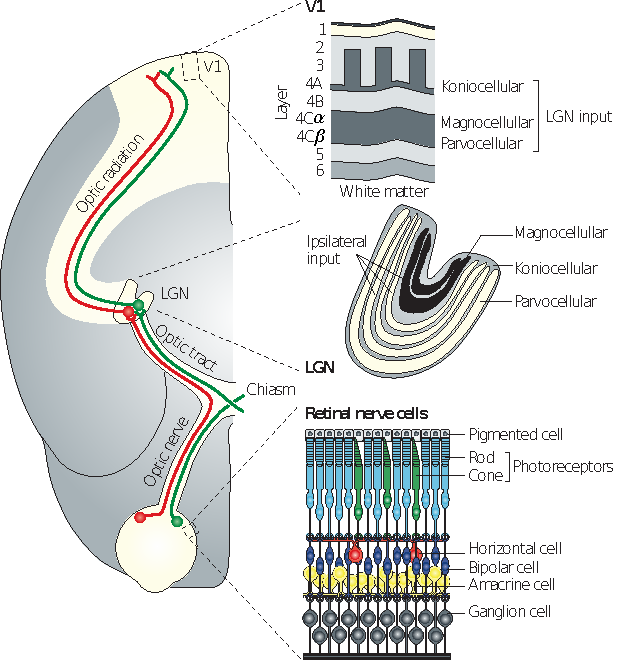
\includegraphics[width=0.9\textwidth]{solomon.pdf}
	\caption{The early visual pathway in primates (at least
          superficially the same for most other mammals) from the
          retina to the primary visual cortex (V1) via the lateral
          geniculate nucleus (LGN) of the thalamus. The left panel
          shows the pathway, while the right panels highlight
          noteworthy sections including the structure of the retina,
          the LGN and V1 broken down into their different layers and
          showing different cell types. Reprinted from
          \cite{Solomon2007}.}
	\label{VisualSystem}
\end{figure}

In the retina, summation of various photoreceptor types gives rise to
so called center-surround receptive fields. These ON- and OFF-center
receptive fields can arise in bipolar cells but are more commonly
associated with retinal ganglion cells (RGCs). This receptive field
type responds most strongly to spots of light/dark moving through the
visual field (as shown in figure \ref{Center-Surround}) but can be
characterized as simple edge detectors.

\begin{figure}
	\centering 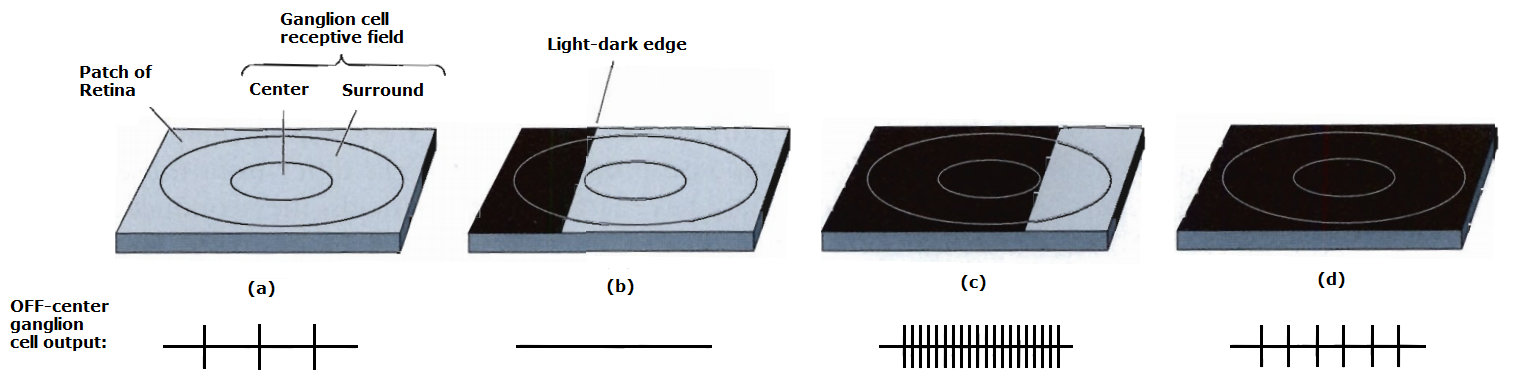
\includegraphics[width=0.9\textwidth]{Figure2.png}
	\caption{The centre-surround receptive field
        structure of some retinal ganglion cells and LGN neurons,
        illustrating how a contrast edge activates different portions
        of the field and thereby results in different activation
        patterns. From left to right one can see that as the
        light-dark edge moves into the ON surround field spontaneous
        activity is suppressed and as it moves further over the OFF
        center field is deactivated causing activity to sharply
        spike. Adapted from \cite{Bear2006}.}
	\label{Center-Surround}
\end{figure}

In addition to the macro-organization of the visual system into
distinct areas the LGN and its downstream structures are further
broken down into individual layers and cell classes. The separation of
LGN cells into layers also corresponds to functional separations, as
layers 1, 4 and 6 usually receive contra-lateral input, while layers
2, 3 and 5 receive ipsi-lateral inputs from the retina. Furthermore,
different layers consist of different cell types, with ventral layers
1 and 2 containing larger so called magno-cellular (M) neurons and
dorsal layers 3, 4, 5 and 6 containing smaller parvo-cellular (P)
neurons with intra-laminar neurons being referred to as konio-cellular
(K). Since these three cell types are also present in the retina and
make connections mainly with their own cell type it is theorized that
each carries its own parallel information stream. Functionally,
P-cells have displayed greater sensitivity to chromatic contrast and
higher spatial frequencies, linking them to the processing of detail
and color, while M-cells have been shown to have greater sensitivity
for high temporal frequencies associating them with motion processing.

\subsection{Primary Visual Cortex: Topographic Maps, Simple and Complex Cells}

The primary visual cortex (V1) or striate cortex provides the first
cortical stage of processing of visual information. The cortex was
classically divided into six layers but since many subdivisions have
been added after functional sub-groups were discovered. Feedforward
input from the LGN is received in layer 4C$\alpha$ and 4C$\beta$ ,
which receive input most of their input from M- and P-cells
respectively. The neurons in layer 4 then send projections up to
layers 2/3, which has a diverse intralaminar network of connections
but also sends intracortical projections to a number of higher visual
areas, while layers 5 and 6 provide feedback to the LGN.

Neurons in the primary visual cortex (V1) are tuned to respond to a
variety of different features or complex combinations of such
features, including orientation, spatial and temporal frequency,
motion direction, colour or ocular origin. In many mammal species
especially primates and carnivores, these feature preferences map
smoothly and topographically onto the cortical surface. This mapping
extends vertically through the layers of the cortex, giving rise to
the notion of distinct cortical columns. Retinotopy arises due to the
mapping of visual information straight from the retina to the LGN and
then to the cortex. Other response preferences such as orientation and
direction selectivity rarely arise in the LGN and are usually thought
of as an emergent phenomenon in the cortex.

\begin{figure}
	\centering 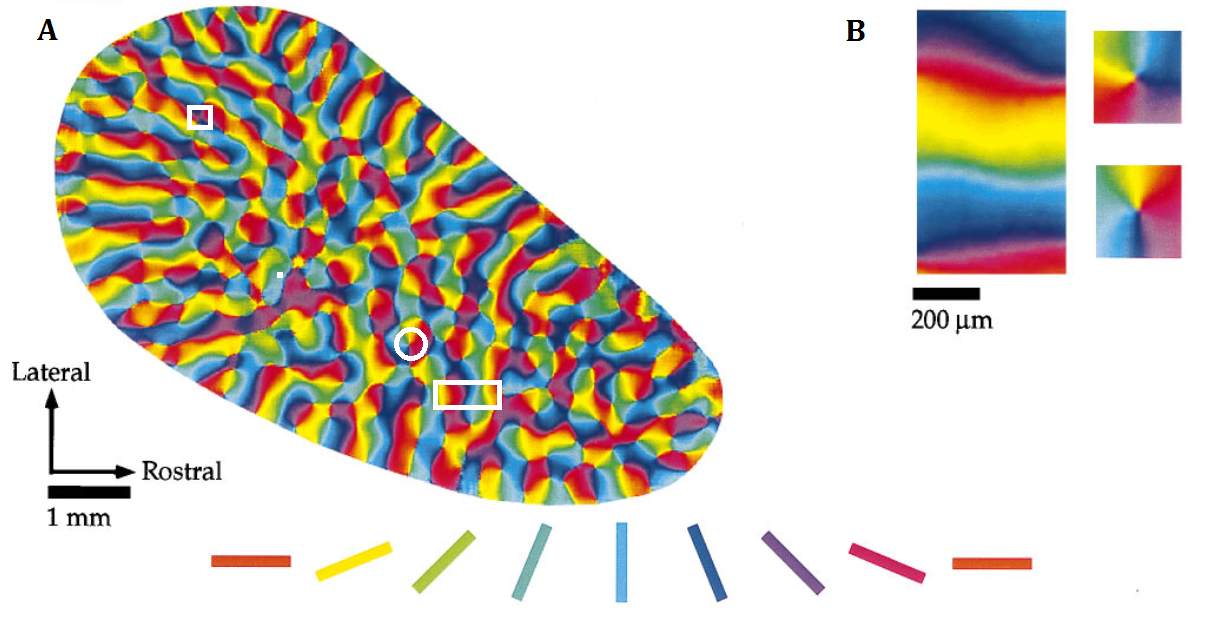
\includegraphics[width=0.9\textwidth]{Figure3.png}
	\caption{A) Orientation preference map in a ferret generated
          by overlaying the activity maps for different orientations
          and artificially colouring each area according to the
          orientation preference laid out in the legend below. The
          image also highlights three recurrent features of
          orientation maps in white. The square highlights a saddle
          point, where a patch of cortex selective for a particular
          direction is almost bisected by a patch selective to another
          direction. The circle highlights a pinwheel arrangement,
          where different orientations preference patches are arranged
          in a circular shape. Finally the rectangular shape
          highlights a linear zone in which orientation preference
          change continuously. B) Magnifications of a linear zone and
          two pinwheel arrangements. Adapted from \cite{Bosking1997}.}
	\label{OrientationMap}
\end{figure}

The receptive fields of V1 neurons are different in that often are no
longer simple ON- or OFF-centre surround fields, forming more complex
spatiotemporal patterns. They are commonly modeled using Gabor filters
as shown in Figure \ref{Gabor}, which have elongated ON and OFF
regions or lobes, generated by localizing a full-field sine grating
with a Gaussian envelope. Orientation selectivity and spatial
frequency preference are determined by the orientation and spacing of
ON- and OFF-regions respectively. It is also possible for V1 cells to
filter temporal patterns by employing spatio-temporal shifts in their
ON and OFF lobes, giving rise to direction selectivity.

Orientation selective neurons can generally be classed as simple or
complex cells, depending on whether they display some form of
spatial/phase invariance. In reality this classification is less clear
with cells being somewhere on a gradient from pure simple cells to a
complex cell with the degree of phase invariance being the determining
factor. Apart from phase invariance the neurons may also exhibit
contrast invariance, such that even at very low contrast they will
respond more strongly to their preferred orientation than to the
orthogonal orientation.

\begin{figure}
	\centering 
\includegraphics[width=0.25\textwidth]{gabor.png}
        
\includegraphics[width=0.25\textwidth]{gabor90.png}
	\caption{Gabor Patches at 0 degree and 90/180 degree
          orientations with clearly visible ON (white) and OFF (black)
          regions.}
	\label{Gabor}
\end{figure}

In context of this project topographic feature maps and RF
interactions play a fundamental role as they provide the basis around
which the neural circuit organize. The functional organization of V1
arises during the development of the animal and are thought to be
mediated largely by activity dependent processes as the next section
will show.

\subsection{Development of Topographic Maps in V1}

The development and maturation of cortical topographic feature
representations in the form of maps is closely linked to function and
can reveal a lot about how the cortex is capable of capturing and
encoding statistics of the natural world. Developmental studies
involve imaging the same area of the cortex over a number of days and
investigating what drives development of orientation maps and other
topographic arrangements. Early developmental studies found, using
relatively limited optical imaging techniques on ferrets shortly after
eye opening, that the iso-orientation domains in the V1 develop very
early in development and subsequently show very little change
\citep{Chapman1996} (pictured in figure \ref{RFMapDevelopment}). These
and other experiments \citep{White2007} showed that orientation
preference develops even in absence of visual input although the maps
do not fully mature. This seems to suggest that orientation maps and
other topographic organizations develop initially even in absence of
external visual input through internally generated visual activity
such as retinal waves but then require external stimulation to fully
mature.

\begin{figure}
	\centering 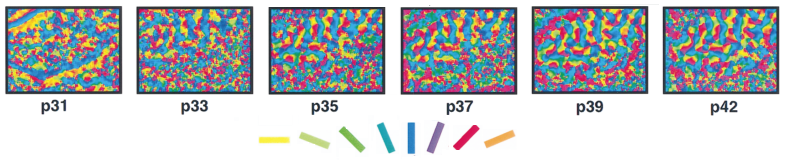
\includegraphics[width=0.9\textwidth]{Figure6.png}
	\caption{Development of orientation map in ferret visual
          cortex from postnatal day 31 to 42 revealed using chronic
          optical imaging of intrinsic signals. Adapted from
          \citep{Chapman1996}.}
	\label{RFMapDevelopment}
\end{figure}

In the initial stages of development various preprogrammed guidance
cues set up the basic connectivity between the LGN and the cortical
processing areas. Some successful models of development have focused
on the afferent connections between the LGN ON and OFF cells and their
targets in the visual cortex as the driving force behind the
development of orientation columns \citep{Jin2011}. This is likely to
tell only part of the story as even during prenatal development,
retinal waves, consisting of periodic activity in retinal ganglion
cells (RGCs), spread across the retina driving neighboring RGCs to
fire in a correlated fashion, which allows the primary visual cortex
to develop topographic feature maps \citep{Firth2005}. The most
prominent proposals in theory and in models have been focused the
termination pattern of both the geniculocortical afferents in layer 4
\citep{Katz2000,Ringach2007} and adjustments in feedforward and
lateral connectivity through activity dependent, competitive processes
\citep{Bednar2003}.

It is now generally accepted that the development of topographic maps
is driven activity dependent weight modification in form of Hebbian
learning or some variant thereof \citep{Wolf}. The LISSOM and
GCAL models, which provide the basis of the modeling work proposed in
this project have shown that robust map development can be achieved
with a small number of relatively simple mechanisms including
homeostatic plasticity, lateral gain control in LGN and lateral
connectivity in V1 \citep{Stevens2013} and will be considered in more
detail at a later stage. These models can account for the development
of orientation preference maps through both intrinsic activity such as
retinal waves \citep{Bednar2003} and visually induced retinal
activity. Experiments show that at the very least these processes are
required to achieve the finely tuned precision, which can now be
observed at single cell resolution \citep{Ohki2005,White2007}.

Lateral intra-areal connections in particular have been implicated in
map development as their functional connectivity seems to be closely
related to map structure \citep{Gilbert1983}. Experiments in layer 2/3
of the tree shrew involving orientation preference mapping and
subsequent axonal staining have shown that although short range
connections show no preference in their terminations, long range
connections longer than 500 \si{\micro\metre}, preferentially link
neurons with co-oriented and co-axially aligned receptive fields
\citep{Bosking1997}. In iso-orientation regions cells therefore make
short-range connections largely with cells that prefer the same
direction as them, while the connectivity at pinwheels short-range
connections are made with cells with a wide range of orientation
preferences \citep{Ohki2006a}. However, it is known that the patchy
lateral connectivity in V1 does not arise until after the orientation
map has emerged \citep{Ruthazer1996}, indicating that they may be
involved in some higher-order processing not required during initial
development.

The development of the early visual pathway is probably driven by a
number of mechanisms complementing each other at various stages
starting with guidance cues setting up coarse predetermined
connectivity patterns, which are then refined through Hebbian
processes driven by in- and extrinsically stimulated
activity. Although the structure of a neurons receptive field is
constantly changing and varies widely from cell to cell, a lot of work
has gone into measuring the exact structure and functional properties
of neural receptive fields and their underlying anatomical correlates,
the neurite arbors.

\section{Developmental models of the Primary Visual Cortex}

As it is thought that the cortex captures statistics about the sensory
streams to construct internal models of the world, it is clear that
function, structure and development are closely linked. Recognizing
this close association, Dr. Bednar began developing models of the
sensory cortex \citep{Bednar2003} based on the original
self-organizing map models (SOM) by von der Malsburg. Since then these
models have been refined substantially but work on many of the same
principles.

The basic idea is that the retina, LGN and V1 are modeled as a set of
neuronal sheets with feedforward and lateral connectivity
self-organizing into the complex topographic maps. These models
provide a very good match to the known developmental timecourse and
replicate a large range of phenomena observed in the mammalian cortex,
yet work with only a small set of mechanism including contrast-gain
control, an adaptive single-neuron threshold, and lateral connectivity
\citep{Stevens2011}. Extensions of this model explaining the development
of complex cells and of contrast dependent size tuning
\citep{Antolik2011} as well as a continuous time model incorporating
LGN/V1 onsets using hysteresis functions are in development
\citep{Stevens2011}.

The GCAL model is based on several core observations about
information-processing in V1 and the cortex in general. As previous
sections have shown, the primary visual cortex of primates responds
strongly to specific low-level features in its visual input including
orientation, color and direction. Selectivity to these features are
conserved across a wide range of contrasts and neurons form
topographic feature maps across the surface of V1 by virtue of
self-organization. While these experimentally confirmed findings are
specific to vision, the concept of equipotentiality proposes that
different areas in the cerebral cortex are cytoarchitectonically
highly similar, becoming differentiated based largely on the
statistical patterns in their inputs during development and are thus
capable of capturing any sensory modality. While details surrounding
this hypothesis are still controversial, experiments such as those by
\cite{Sur1990} have at least partly validated this view. In this
particular study, experimentalists rewired optic nerve axons to
interface with neurons in the medial geniculate nucleus (MGN), part of
the pre-cortical auditory pathway, and subsequently showed that
neurons in the primary auditory cortex (A1) would become receptive to
features usually associated with V1. This is behind much of what has
made V1 such a popular model area for neuroscience and suggests that
many of the insights that can be gleaned from the study of V1 could be
applied to the cortex as a whole.

\begin{figure}
	\centering 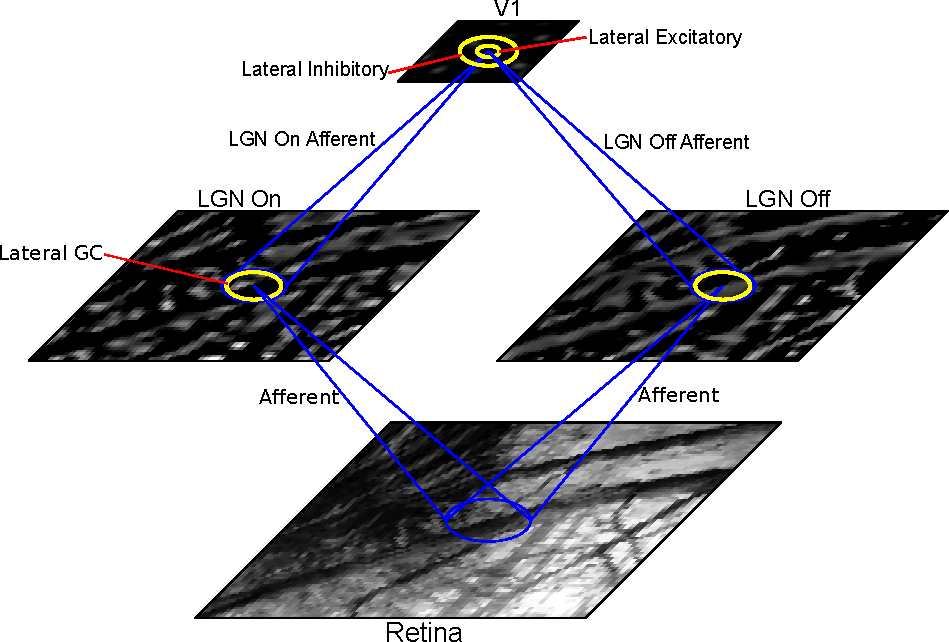
\includegraphics[width=1.0\textwidth]{GCAL.pdf}
	\caption{Schematic of simplest GCAL model for development
        of simple cells with surround modulation, retinotopic
        organization and orientation preference maps. It consists of a
        retinal sheet, two RGC/LGN for ON and OFF cell responses and
        one V1 sheet, connected with intra- and inter-areal
        projections. The sheets are drawn to scale, with larger sheets
        for the RGC/LGN and retinal layers to avoid edge
        effects. Projections are illustrated with blue (feedforward
        connections) and yellow (lateral connections) ovals with cones
        converging on their target, all drawn to scale to show their
        spatial extents. RGC/LGN sheets consist of units with
        hardwired Difference of Gaussian RFs with ON and OFF
        center-surround regions. LGN Afferent projections to V1 are
        initially unspecific but develop Gabor-like RF structures
        through Hebbian learning as they are observed experimentally.}
	\label{GCAL}
\end{figure}

The architecture of the GCAL model in its simplest form and as it will
initially be used in this project relies on only four sheets, a
retinal sheet for the presentation of stimuli, two RGC/LGN sheets and
a V1 sheet. These sheets are connected with different intra- and
inter-areal connection fields. This simple model can only be used to
demonstrate retinotopy, orientation preference and the emergence of
simple cell-like RFs but more complex models have been shown to
additionally account for complex cells, ocular dominance, motion
direction, spatial frequency, temporal frequency, disparity and
color. All these models are trained by presenting it with a visual
input on the retina, allowing the response to propagate through the
different sheets and then adjusting the connections weights to V1
neurons based on a local learning rule. The response of a given neuron
$j$ at time $t+\delta t$ can be calculated as the thresholded dot
product between the activations of every input neurons $i$ at time
$t$, or $\eta_i(t)$, and their associated weights stored in the
connection field:

\begin{equation}
\eta_j(t+\delta t) = \sigma \left ( \sum_p{\gamma_p} \sum_{i \in
  F_{jp}}{\eta_i(t)\omega_{ij}}\right)
\end{equation}

where $\eta_i$ is the activation of all units $i$ in connection field
$F_{jp}$, which contains all neurons unit $j$ receives its inputs
from. $\omega_{ij}$ is the connection weight from $i$ to $j$. $\sigma$
is a half-wave rectifying function with a variable threshold point
($\theta$) dependent on the average activity of the unit, effectively
acting as a homeostatic mechanism, pulling the activity of neuron back
to a desired level. $\gamma_p$ is an arbitrary multiplier for the
overall strength of all connections $i$ in projection $p$ and thus a
free parameter.

The connection weights $\omega_{ij}$ are adjusted after each iteration
using a simple Hebbian learning rule, capturing correlations between
pre- and post-synaptic activities. The Hebbian connection weight
update for unit $j$ is expressed as a function of the presynaptic
activity $\eta_i$, the post-synaptic response $\eta_j$ and the Hebbian
learning rate $\alpha$, taking the form:

\begin{equation}
\omega_{ij}(t+1) = \frac{\omega_{ij}(t) + \alpha \eta_j
  \eta_i}{\sum_{k\in F_jp}{ (\omega_{kj}(t) + \alpha \eta_j \eta_k)}}
\end{equation}

This function also constrains runaway changes in weights by employing
divisive post-synaptic weight normalization and thus eliminates the
instability associated with classical Hebbian learning.

This limited number of mechanisms already gives rise to an incredibly
robust model of development of topographic map development and
generates different experimentally observed RF profiles. To add
further robustness to the model and to allow it to respond across a
wide range of contrasts, contrast-gain control was introduced in the
LGN sheets (marked as Lateral GC). This mechanism was closely modeled
on the divisive normalization model introduced and validated by
\cite{Bonin2005}. Finally, the lateral excitatory and inhibitory
fields in the V1 sheet give rise not only to the topographic map
structure but also to some surround modulation effects. In particular,
it can explain the size tuning properties of V1 neurons as the
excitatory field will boost the response to a growing centered disk up
to a certain peak, after which point the lateral inhibitory field
dominates and reduces the response to the stimulus as it grows
further. It may also explain effects such as iso-orientation
suppression but this has as of yet not been explored in detail.

Overall, due to the simplicity of its mechanisms and its explanatory
strength, GCAL provides an ideal starting point to explore the
contribution of feedforward, lateral and feedback components to V1,
how bottom-up attention can arise and how top-down attention can
modulate the processing architecture.

\subsection{Functional and Anatomical Properties of Neural Receptive Fields}

The spatial properties of RFs in the LGN and V1 are of particular
interest in the context of this thesis as they provide the basis of a
realistic model of the para-foveal regions of the primary visual
cortex in macaques, allowing direct comparisons between model in
experiment in a system where the spatial scales are of great
importance. Before attempting to model the recurrent, lateral inputs
to V1, the spatial properties of each set of afferent connections
entering V1 need to be thoroughly understood and incorporated into the
model.

The extents and structure of neural receptive fields are defined by
the axonal and dendritic arborization of afferent, horizontal and
feedback connections, whether that is in the LGN, the V1 or higher up
in the cortical architecture. While these extents can theoretically be
measured physically by tracing the neurites of a number of cells, this
has only systematically been possible for corticogeniculocortical
neurite complex as tracing studies along the retinal-geniculate
pathway are generally infeasible. Therefore spatial properties of LGN
RFs have been estimated through stimulus driven protocols. The
following sections will outline the methods employed in characterizing
geniculate RFs and detail the relative contribution of afferent,
lateral and feedback connections to para-foveal RFs in the LGN and V1
of macaques.

\subsubsection{Receptive Fields in the Lateral Geniculate Nucleus}
\label{sec:LGNRF}

The spatiotemporeal structure of receptive field becomes increasingly
more complex when moving up in the visual processing hierarchy. As
described earlier, receptive fields in the LGN are primarily made up
of antagonistic center-surround regions although Gabor-like lobes are
also sometimes observed. Even at this early stage of processing,
lateral and feedback connections can modulate neural responses and
have been found to exert a suppressive effect \citep{Hubel1961}. More
recent studies have concluded that this suppressive effect is mediated
primarily by lateral connections and acts as a form of contrast-gain
control allowing for the encoding of a high dynamic range of luminance
values \cite{Bonin2005}. As pointed out previously the LGN receives a
large proportion of its inputs from feedback cells originating in
layer 6 of V1 \citep{Sherman2002}. It is unclear how these feedback
connections contribute to the RF properties of LGN neurons but most
evidence suggests they are mainly involved in higher level modulatory
processes especially in regard to the processing of motion and thus do
not directly contribute to the RF structure \citep{Sillito2006}.

Estimating the relative contribution and effect of the various LGN
afferents on its neural receptive fields has been attempted using a
variety of protocols. Unfortunately little to no data is available
from tracing studies, primarily because the LGN is embedded deep in
the brain making it incredibly difficult to trace individual neurites
from and to their origin. Therefore a number of protocols were
developed by which the parameters of the center-surround fields could
be estimated. After measuring the response of retinal ganglion cells
(RGCs) to moving bar stimuli cats \citep{Rodieck1965a,Rodieck1965b},
\cite{Rodieck1965} found that by fitting a Difference of Gaussian
(DoG) model (see \ref{DoGf}) to the data it was possible to estimate
the relative strength and size of the central and surround portions of
the receptive field. It wasn't until later that systematic recordings
of this kind were carried out in the LGN of macaques at which point
the moving bar stimuli were replaced with sine gratings of varying
spatial frequency.

\begin{equation}
R = k_c e^{-\frac{f}{f_c}^2} - k_s e^{-\frac{f}{f_s}^2}
\label{DoGf}
\end{equation}

As not all papers can be considered, the data from three different
studies making use of protocols with increasing complexity will be
considered. \cite{Derrington1984} was the first of such studies,
attempting to characterize the spatial and temporal properties of
parvocellular LGN neurons in \emph{Macaca mulatta} by fitting DoG
models to the responses. The analysis and confidence intervals of this
first study were rather limited so the first study that will be
considered here is \cite{Spear1994}, which also considered the effect
of aging on receptive field properties. They found that the receptive
field center radius only increased very weakly with eccentricity, the
smallest RF center radii were confined to parvocellular neurons and
that the RF surround was significantly smaller in parvocellular
layers. This provides a first estimate for the mean sizes of the
central and surround portions of the classical RFs in macaque but the
clear problem with this approach is that it completely ignores the
influence of the non-classical surround and therefore may
underestimate the extents of the central field, while overestimating
the strength of the classical RF surround.

The next detailed study of LGN neural RFs was carried out by Levitt et
al. \cite{Levitt2001}, investigating the effects of visual deprivation
on their visual response properties. The study additionally set out to
determine the trans-species correspondence of so called X, Y and W
pathways, which were identified in the cat. As in the \cite{Spear1994}
study they found little difference in RF center radii between parvo-
and magnocellular neurons. They also found that magnocellular neurons
had greater nonlinearity indices but could find no compelling evidence
that magnocellular neurons can be classified into distinct linear (X)
and nonlinear (Y) types. There was a tendency for parvocellular
neurons to exhibit greater spatial resolution and the highest temporal
resolution to be magnocellular. This seems to support the general
conclusion reached by \cite{Derrington1984}, which had additionally
concluded that magno- and parvocellular neurons can be further
identified by their chromatic properties.  Finally, their analysis
extended to earlier data from different species of macaque, which
showed that there is some variation in the distribution of ON and OFF
cells between \emph{M. mulatta} and \emph{M. fascularis}. Overall
their results on spatial tuning match those found by previous studies
quite closely, which is unsurprising as the measuring and fitting
protocols were highly similar.

In an attempt to calculate the relative contributions of different
neural connections, determine differences between the K-, M- and
P-cellullar pathways and measure contrast dependent tuning, a number
of more recent studies have introduced more complex measurement and
fitting protocols. In particular, these experiments for the first time
attempted to separate out the influence of the non-classical or
extra-classical surround (ECRF or nCRF), which is thought to be
mediated by lateral and feedback connections. Therefore, a new
measurement and fitting protocol, introduced by \cite{Sceniak1999} in
form of the integrated DoG (iDoG) model to describe spatial summation
in the visual cortex, was used. Instead of measuring the response to
varying spatial frequency, this protocol involves the presentation of
drifting sine grating disks with varying apertures at the neurons
optimum spatial frequency. The rationale behind this new protocol was
that the optimal spatial frequency would maximally drive the CRF
excitatory center, while minimizing the influence of the CRF
surround. Therefore the resulting area summation tuning curve would
represent only the response from the CRF excitatory center and the
ECRF surround. Additionally the spatial frequency response measurement
protocol was modified by confining the drifting sine gratings to a
circular aperture, reducing influences from beyond the CRF. While
these assumptions do not necessarily hold for reasons that will be
discussed later, they provide a first systematic attempt at separating
the contributions from the CRF and ECRF.

\cite{Sceniak2006} were the first to study spatial RF properties of
LGN neurons of macaques by measuring both spatial frequency and area
summation response functions and fitting the results with DoG and iDoG
models respectively to estimate the spatial parameters of the probed
neurons. These results represent the best estimates of the spatial
properties of LGN receptive fields. The first thing to note is the
clear discrepancy between the estimates of CRF excitatory center
radius estimates in this paper compared to previous estimates. This
may be explained by the more homogenous distribution of cells as the
sample population was taken exclusively from layer 4. Additionally the
older protocol failed to confine the drifting sine grating to a disk,
which may have resulted systematic underestimation of the excitatory
component due to suppressive effects. While excitatory extents vary
hugely across the various studies the suppressive surround estimates
are fairly consistent. Furthermore, the spatial extent of the
excitatory CRF centers were found to be contrast invariant, while both
the ECRF and CRF suppressive surround extents were found to increase
at lower contrast levels. In summary, looking back at all the studies
considered here excitatory CRF extents are generally distributed
between 0.05-0.5$\degree$ in radius, while inhibitory CRF and
suppressive ECRF radii are distributed distributed anywhere between
0.6-1.5$\degree$ and the suppression index is quite high
(SI\textgreater0.8) for 80\% cells.

While these results provide the best estimates that are currently
available the protocols used rely on a number of flawed
assumptions. The DoG model fitted to the spatial frequency tuning
curve relies on the assumption that no other components are
contributing to the response. Although the limited size of the sine
grating disk drive should reduce long range influences on the response
and the ECRF surround is frequency invariant over a broader spectrum
than the CRF, further contributing mechanisms cannot be excluded and
may therefore affect the estimates. Similarly the iDoG model fitted to
area summation tuning curves may be affected by a number of
unaccounted mechanisms. Additionally the iDoG model (see \ref{iDoG})
actually corresponds to an even luminance disk of variable size rather
than the sine grating disks that were used by \cite{Sceniak2006}. The
decision to use technically incorrect stimuli was made to minimize the
influence of the inhibitory CRF surround, which may itself still have
some influence on the response. While all these limitations should be
held in mind, it is still the best attempt at controlling unaccounted
contributions and thus provides the best data on the spatial
properties of macaque LGN RFs until detailed histological studies
become feasible.

\subsubsection{Receptive Fields in the Primary Visual Cortex}

The receptive field properties of neurons in V1, in contrast to LGN
neurons, have been characterized to a far greater extent with a number
of studies publishing direct anatomical data on neurite arborization
in addition to studies involving stimulus protocols such as those
employed to characterize LGN RFs. A number of reviews have been
published in the past decade to classify different portions of the
receptive field and link them to their physiological substrate in the
form of feedforward (FF), lateral and feedback (FB) connections. In
order to attain a proper understanding of the spatial distribution of
afferent neurites, populations of V1 neurons are targeted by, this
section will summarize the results.

Recent analyses have established a more complex model for the
classification of the spatial properties of neural RFs in V1 than the
simpler classical and extra-classical RF structure utilized in earlier
work. The structure of a V1 receptive field has been visualized by
\cite{Angelucci2006a} and can be seen in Figure \ref{RFstruct}. It is
broken down into the minimum response field (mRF), the summation
response field (sRF), which itself is broken down into the high
contrast and low contrast summation RF (hsRF and lsRF) and the far
surround. In particular, a distinction has been made between the near
surround, which extends as far as the lsRF and a suppressive far
surround that extends beyond the lsRF. The distinction between the
hsRF and lsRF has been introduced to account for the contrast
dependence of size tuning. Problematically not all studies nor even
all the latest studies use this means of defining different portions
of the RF, which may have led to discrepancies of how the sizes of
different RF areas are reported. The following sections will attempt
to integrate the results from studies employing different means of
classifying RFs.

The studies reviewed in \cite{Angelucci2006a} seem to indicate that
geniculocortical FF projections integrate signals in the hsRF, while
lateral connection underly the lsRF and may thus account for the
contrast dependence of spatial summation as well as modulatory effects
in the near surround. Classification through measurement of spatial
dimensions and onset latencies indicate that inter-areal FB
connections seem to be responsible for modulatory influences from the
far surround. The influence and spatial properties of each of these
projections will be detailed in the following sections.

\begin{figure}
	\centering
        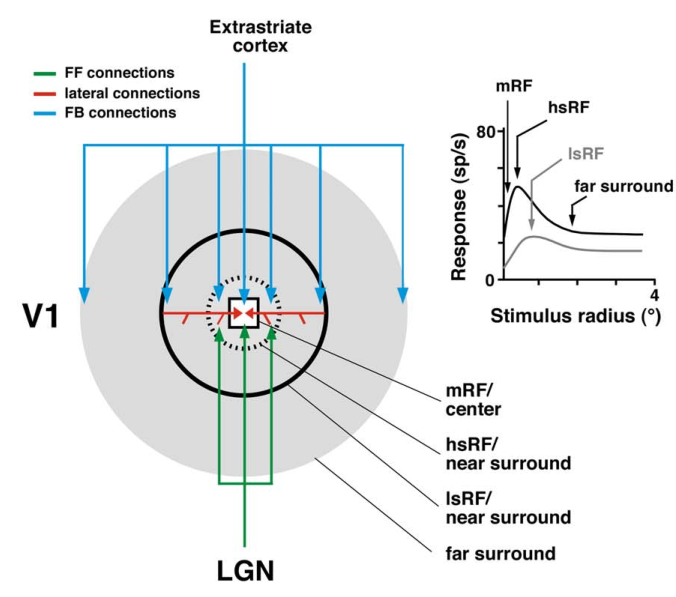
\includegraphics[width=1.0\textwidth]{angelucci_RFstruct.pdf}
	\caption{The receptive field structure of V1 neurons
        showing the minimum receptive field (mRF), high contrast
        summation RF (hsRF) and low contrast summation RF
        (lsRF). Taken from \cite{Angelucci2006}.}
	\label{RFstruct}
\end{figure}

\paragraph{Geniculocortical Afferents and the Minimum and High Contrast Summation RF}

The primary visual cortex receives most of its driving inputs through
the three previously detailed M-, P- and K-cellular geniculocortical
pathways. The M-pathway principally terminates in layers 4C$\alpha$
and 6, the Parvocellular afferents terminate in layers 4A, 4$\beta$
and 6, while K-cells primarily target layer 1 and some regions of
layer 3. By combining anatomical-tract tracing with physiological
recording the spatial extents of feedforward connections have been
measured in detail and linked back to the different RF regions.

The minimum response field as defined above is commensurate to the
classical RF and is usually mapped using drifting gratings masked to a
small disk of optimal parameters for that particular neuron. It is
surrounded by the high contrast summation RF, which is measured by
increasing the size of a drifting grating disk at high contrast until
the neuron reaches its peak response. Using a combination of tracing
and electrophysiological recording \citep{Angelucci2006a} found that
the visuotopic extent of LGN afferents matches the hsRF size of the
target V1 neuron. The diagram and bar chart in Figure \ref{FFmatch}
show how closely the estimates from tracing studies match the results
from physiological classifications of RF areas for magno- and
parvo-cellular pathways. The close match between these different
experiments suggests geniculocortical afferents may underly the extent
of a V1 neuron's mRF. Recent evidence has also shown that the an LGN
neurons hsRF is roughly commensurate with a V1 cell's mRF. This seems
to suggest that the mRF of V1 cells is a product the summation of LGN
cells at their peak spatial summation, while the hsRF region of V1
neurons is defined by the integration of excitatory inputs from
partially suppressed LGN cells. Beyond that it seems likely FF
components partially contribute to surround suppression in V1, however
the spatial scales of surround modulation as well as its orientation
specificity seem to rule out LGN afferents as the major contributor to
the modulatory surround \citep{Angelucci2002,Angelucci2006a}.

\begin{figure}
	\centering
        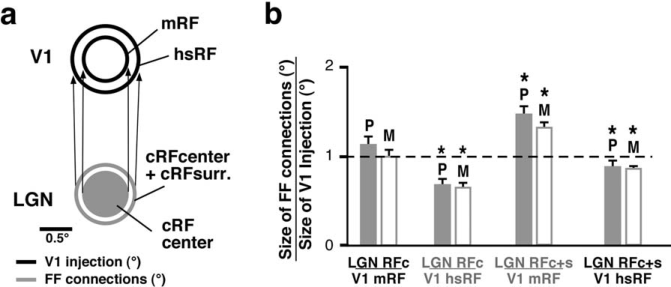
\includegraphics[width=1.0\textwidth]{angelucci_RFmatch.pdf}
	\caption{Comparisons between electrophysiological
        characterisation of RF structure and the spatial structure of
        geniculocortical projections to V1 in (a) diagramatic and (b)
        chart form. Both demonstrate that the mRF and hsRF are
        coextensive with the spatial extents of geniculocortical
        afferents to V1. Taken from \cite{Angelucci2006}.}
	\label{FFmatch}
\end{figure}

Having established the contribution of geniculate afferents to the RF
of V1 neurons its time to look at their spatial distribution. In their
extensive studies and culminating review paper, Angelucci et al.
\cite{Angelucci2006} first fitted the iDOG to the spatial summation
response curve of a number of V1 neurons, injected the recording sites
with tracers and then measured the labeled connections and cell
bodies. The linear extents of the labeled connections were converted
to visual field coordinates using magnification factor (MF) estimates
by \cite{VanEssen1984}. Additionally the anatomic extent of the label
was measured in LGN and again converted to visual space coordinates
using MFs measured by \cite{Connolly1984} and LGN RF size estimates by
\cite{Derrington1984}. These calculations were used to arrive at the
aggregate receptive field (ARF) size, which takes the form:

\begin{equation}
  ARF_{deg} = D^{\degree} + RF_{mean}
\end{equation}

where $RF_{mean}$ is the mean RF size of cells recorded at the edge of
the injection site, which could reflect the mRF, hsRF or lsRF, and
$D^{\degree}$ is defined as:

\begin{equation}
  D^{\degree} = D_{mm} / MF_{mm/deg} + S_{deg}
\end{equation}

where $D_{mm}$ is the diameter, $MF_{mm/deg}$ is the magnification
factor and $S_{deg}$ is the RF scatter at the injection site. The
results show a close match between mRF and hsRF sizes as estimated in
V1 and sizes of the RF center and RF center + surround as measured in
LGN, once again reaffirming the idea that the mRF and hsRF are
primarily driven by geniculocortical afferents. The latest review
\citep{Angelucci2006} has measured the size of the hsRF in V1 neurons
of macaques at 2-8$\degree$ eccentricity as having mean of about
1$\degree \pm$ 0.1, which is roughly 2.2x larger than the mRF of the
same cell based on results from \cite{Angelucci2002} and
\cite{Levitt2002}. Estimates from the latest anatomical study
summarized in table \ref{V1_histology} provides slightly higher
estimates with means of 1.09$\degree$ and 1.41$\degree$ in layer
4C$\alpha$ and 4A/C$\beta$ respectively.

In addition to the spatial extents of V1 RFs, \cite{Angelucci2006a}
also estimated the number of LGN afferents that would contact an
individual V1 neuron. According to their estimates a single neuron in
layer 4C$\alpha$ can be expected to receive roughly 11 projections
from LGN M-cells. Although they were not able to put their own
estimates to the Parvocellular pathway, based on anatomical data from
cats they determined that on average 10 geniculate cells converge on a
V1 layer 4 cell having observed only a maximum of ~30. They conclude
that the geniculocortical pathway in macaques exhibits an even lower
level of convergence than in cats.

In summary, evidence from anatomical and electrophysiological data
seems to suggest that the hsRF of V1 neurons and by proxy the
geniculocortical afferents are on average between 1.0-1.5$\degree$ in
size, exhibiting highly limited convergence with only about 10 cells
targeting a single layer 4 V1 cell.

\paragraph{Lateral Connections and the Low Contrast Summation RF}

Horizontal, lateral or intra-areal connections have been proposed as
the mechanism for a number of observed phenomena, including the
contrast dependence of size tuning, which is why it is thought they
underly the extent of the lsRF. Classically it has been assumed that
lateral connectivity manifests itself through short-range excitatory
and long-range inhibitory connections
\citep{VonderMalsburg1973,Obermayer1990b}. More recent studies have
indicated that intra-laminar projections usually originate in
excitatory pyramidal neurons in layers 2/3, 4B, upper 4C$\alpha$ and
5/6 and at least in layers 2/3 have been shown to target ~80\%
excitatory and ~20\% inhibitory neurons. The spatial scale of these
connections has led several studies to conclude that they may mediate
modulation of RF center properties in the near surround
\citep{Angelucci2002}. Lateral connection could therefore provide a
simultaneous mechanism for a number of observed effects including the
expansion of the summation RF at low stimulus contrast
\citep{Sceniak1999}, colinear facilitation \citep{Mizobe2001} as well
as suppression from the near surround outside the hsRF but within the
lsRF \citep{Sceniak2001,Levitt2002}. The previous section showed that
such phenomena could not be adequately accounted for by
geniculocortical afferents, measurement of spatial extents and
response latencies of horizontal connections reaffirm this view and
have shown that the lsRF and lateral connections are coextensive
\citep{Angelucci2002}.

Apart from the exact spatial dimensions of horizontal connections, it
is important several other functionally important properties. While
layer 2/3 neurons display patchy connectivity, linking regions with
similar functional properties such as orientation preference or ocular
dominance, this has been shown not to be the case in macaque layer 4B,
upper 4C$\alpha$ \citep{Angelucci2002}. In addition, it was found that
horizontal connections in macaque V1 are isotropic in visual space
unlike the anisotropy along the axis of preferred orientation observed
in tree shrews \citep{Bosking1997} and several other species. This may
also indicate that contour completion in macaques is mediated by
feedback connections. Horizontal connections have been shown to
illicit only subthreshold responses \citep{Hirsch1991} and are thus
limited to modulatory influence. However, as the surround modulation
extends far beyond the monosynaptic spread of lateral connections it
is unlikely they account for modulation from the far
surround. Polysynaptic chains of lateral connections are also an
unlikely substrate for the far surround due to the slow conduction
velocity of their axons. In particular, \cite{Bair2003} showed that
onset latencies of suppression from the far surround were almost equal
to the delays from the near surround. This makes it likely that far
surround modulation is mediated primarily by inter-areal feedback
connections, which we will look at in detail at a later stage.

Having established that spatial profile of lateral connections is
commensurate to that of the lsRF and vice versa the data from both
sources will be laid out and analyzed. Anatomic data suggests that the
spatial spread of lateral connections can be anywhere between 3-10 mm
(on average 6-7 mm) in total length \citep{Angelucci2002}, which is
broken down by layer in table \ref{LatExtents}. Along its principal
axis the visuotopic monosynaptic spread of V1 horizontal connections
has a mean of $2.47\degree \pm 0.3\degree$. This falls well within the
range of estimates for the lsRF as published in a number of studies
\citep{Shushruth2009,Sceniak1999,Sceniak2001}, which were fit with the
same integrated DoG model and stimulus protocol as used in the
\cite{Sceniak2006} paper on the spatial properties of LGN neurons,
reviewed previously.

In summary, there is strong evidence that lateral connections underly
the extent of the lsRF and mediate a number of effects in the near
surround, including contrast dependent size tuning, colinear
facilitation and low contrast suppression. Unlike in other species
horizontal connections are isotropic but do exhibit patchy
connectivity in layer 2/3. The extents of horizontal connections range
between 3-10 mm, which averages to around 2.5$\degree$ in visual
space.


\paragraph{Feedback from Higher Cortical Areas and the Far Surround}

As the previous to sections have shown, modulatory influences to V1
RFs extend well beyond the spatial spread of both geniculocortical
afferents and horizontal connections. This extended modulatory field
is known as the far surround and is thought to be mediated by feedback
from higher cortical areas. The far surround has generally been
characterized as suppressive, especially for iso-oriented gratings in
the center and far surround. More detailed analysis has shown that the
far surround can also exhibit response facilitation under some
stimulus conditions. This section will characterize the function,
termination patterns and spatial extents of feedback connections from
higher cortical areas to V1.

The notion of a hierarchical organization of cortical visual areas has
been around for quite some time and more recent analysis of
feedforward and feedback connections has affirmed this view. At the
bottom of this hierarchy is V1, sending partially segregated FF
projection to areas V2, V3, V4 and visual area middle temporal (MT),
which all send FB projections back to V1
\citep{Felleman1991}. Feedforward projection from V1 to V2 arise
mainly from layer 4B and to a lesser degree from layer 2/3 and
6. Feedback connections on the other hand arise from layers 2/3A and
5/6 and terminate in the same layers from which FF connections are
sent, which means the cells projecting up the hierarchy often overlap
with the termination regions of FB projections being sent back down
\citep{Angelucci2002}.

Just like lateral connections FB connections do not drive their target
cells, exhibiting only modulatory influence on the RF center
\citep{Bullier2001a}. Inactivation of areas V2 and MT has been shown
to reduce the firing rate of V1 neurons to stimuli in their RF center
\citep{Hupe1998}, suggesting FB inputs are summed with FF inputs to
increase activity. The exact balance between excitation and inhibition
of FB connections is so far not very well explored in macaques but
evidence from rats suggest that they almost exclusively target
excitatory cells. However \cite{Angelucci2006} and \cite{Schwabe2006}
have proposed a regimen where FB connections in the far surround
target pyramidal neurons, which in turn send monosynaptic horizontal
connections to excitatory and inhibitory neurons in the RF center and
can thus mediate both suppressive and facilitatory effects depending
on stimulus properties.

Feedback connections have been thought to underly a number of top-down
effects in V1, including attention \citep{Treue2003}, the reverse
hierarchy theory of visual learning \citep{Ahissar2004} but more
recent studies have suggested they contribute directly to the response
of V1 neurons to simple visual patterns
\citep{Angelucci2002,Angelucci2003,Schwabe2006}. Notably
\cite{Schwabe2006} and \cite{Ichida2007} seem to have resolved the
conflicting evidence about the far surrounds suppressive and
facilitatory role. Using both experimental and theoretical work they
found that while the far surround is suppressive under high contrast
conditions, the response of a neuron to a low contrast stimulus in the
RF center is facilitated by a small annular stimulus in the far
surround. This indicates that excitatory and inhibitory surround
mechanisms have similar extents and that the sign of their
contribution depends on changes in local excitation/inhibition balance
brought about by surround stimulation.

The spatial and functional organization of the FB pathway is thought
to differ significantly from FF connections. They seem to exhibit less
precise retinotopic organization and terminate in a more diffuse
fashion than FF connections. However, more recent evidence suggests
that at least a subset of FB connections exhibit patchy and
functionally specific termination patterns
\citep{Angelucci2006}. Evidence from new world primates has also shown
that V2 FB axons to V1 link regions of similar orientation preference
and that their terminal fields are anisotropic along the axis of the
preferred orientation of the originating cell in V2
\citep{Shmuel2005}. The discrepancy between different studies in
finding diffuse and patchy FB termination patterns may be attributable
to different labeling methods and given that CTB labeling is the more
mature and tested procedure it seems likely that FB connections do
exhibit patchy terminations in layers 1B, 2/3, 4B and 5/6 and diffuse
terminals in layer 1A. The observation of patchy connectivity is also
consistent with their proposed functional role in mediating
feature-specific influences from the far surround.

The anatomical spatial extents of FB connections from higher cortical
areas have been measured in a number of tracing
studies. \cite{Angelucci2002} provides a measurements broken down by
area, measuring the extents of FB connections from V2, V3 and MT to V1
(see table \ref{FBExtents}). Once converted into degrees of visual
space the results are the following: Feedback from V2 has a mean size
of 3.4$\degree$ in layer 2/3 and 3.8$\degree$ in layers 5/6, FB from
V3 a mean size of 5.6$\degree$ in layers 2/3 and 6.7$\degree$ and FB
from MT a mean size of 15.3$\degree$ and 26.6$\degree$ in the upper
and lower layers respectively. The largest far surround field measured
was 28$\degree$ in diameter and the measurement was still limited by
the maximal presented stimulus size \citep{Ichida2007}. These results
clearly indicate that cortical feedback to V1 increases in its spatial
extents and becomes less spatially and retinotopically specific when
moving up in the cortical hierarchy to the point where it covers huge
portions of the visual field, trading spatial specifity for
specificity for more complex features.

Feedback projection from higher cortical areas to V1 mediate a number
of important contextual effects and has been implicated in the early
stages of visual attention but also seem to be closely involved in the
processing of simple visual stimuli. This section has summarized
current knowledge on the spatial termination patterns of FB
connections to V1, indicating how they could give rise to functional
properties of V1 information processing. While this information will
aid the development of a strongly constrained model, without an
understanding of the information content being fed back to V1 from
higher cortical areas understanding of their true function will be
limited.

\section{The Internal Circuitry of Striate Cortex}

The previous section outlined the overall structure of the early visual
system, breaking down the contribution of inputs from various sources
on the receptive field (RF) of neurons in primary visual cortex
(V1). While this provides general anatomical constraints and sheds
some light on the functional circuitry underlying many of the
contextual effects that have been observed in the primary visual
cortex, it does not address many of the fundamental questions about
the functional significance of recurrent cortical processing. In
particular, it does not address the delicate balance in both strength
and spatial extent between excitation and inhibition that is required
to halt runaway excitation, sparsify the inputs and thereby allow for
the formation of concentrated activity bubbles around which
self-organization can take place. This section will cover how the
understanding of intra-cortical connectivity has evolved and how this
has been reflected in various developmental and non-developmental
models.

\subsection{The Mexican Hat}

Before complex tracing and circuit reconstruction techniques became
available, considerations about the connectivity profiles in the
cortex were largely theoretical or based on data from other anatomical
structures, which were at the time more amenable to study. Anatomical
data and electrophysiological studies in the retina had shown that
there is a strong lateral inhibitory component involved in
decorrelating photoreceptor activities, thereby enabling more
efficient coding of the input \citep{Atick1992}. Lateral inhibition
was taken to be a general principle of sensory systems and, among
others, \cite{Blakemore1970} suggested repulsive interactions between
neighboring contours could account for psychophysical data. Further
evidence of lateral inhibition as a general feature of sensory systems
was provided by a variety of theoretical models of self-organization,
highlighting the necessity of effective local excitatory and long
range inhibitory interactions for the formation of local activity
bubbles, which in turn provided the basis for orderly map organization
\citep{VonderMalsburg1973,Miller1989}.

The connectivity profile employed in the various self-organizing map
models became known as the Mexican hat profile due to its strong
resemblance to a sombrero. A simulated Mexican hat profile is shown in
\ref{MexHat} generated through a simple difference of Gaussian (DoG),
whereby a small positive Gaussian kernel is combined with a larger
inhibitory kernel. A large variety of cortical models have
successfully employed this connection profile to explain a variety of
effects ranging from topographic map organization, orientation tuning
and contextual effects. Problematically, it is unclear how
biologically realistic the assumption of strong local excitation and
broadly tuned or untuned inhibition is.

\begin{figure}
	\centering 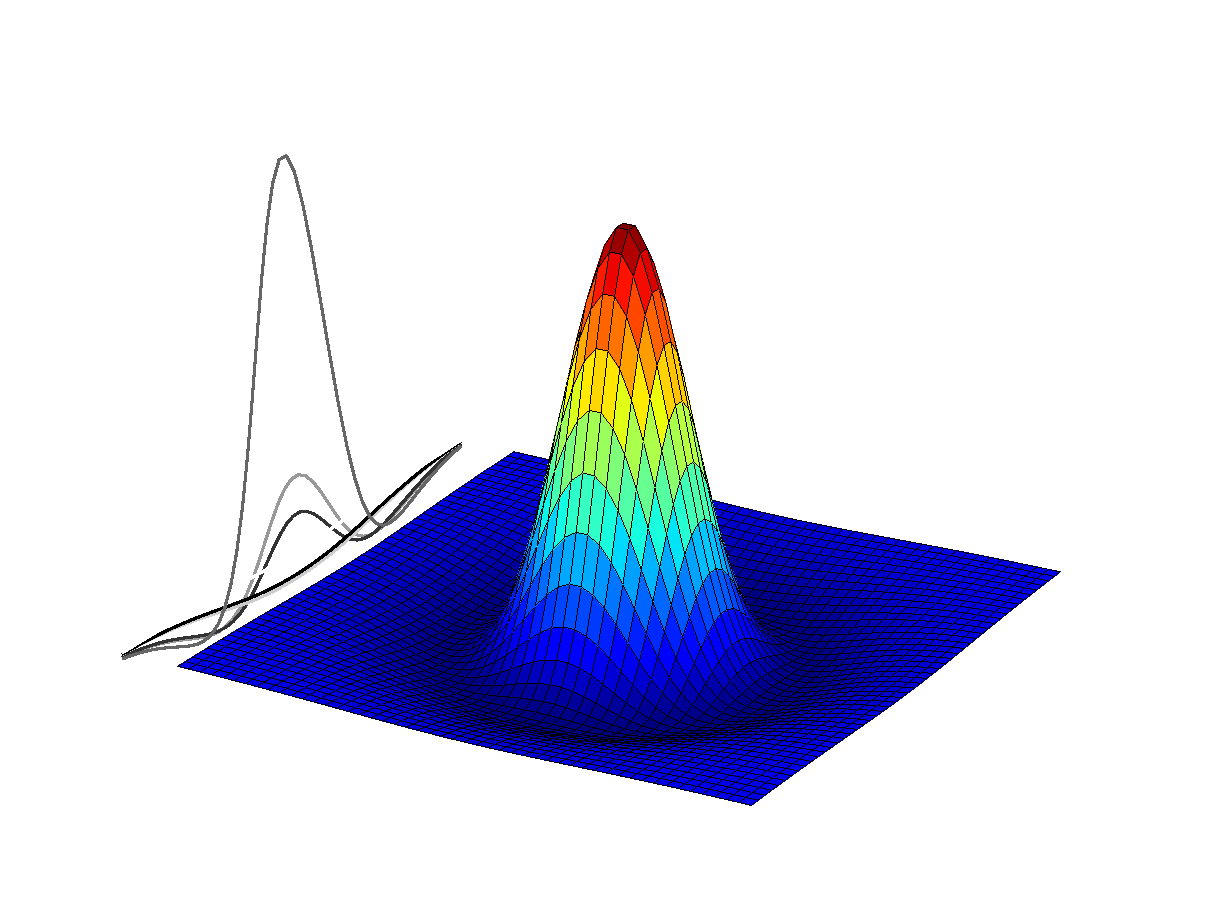
\includegraphics[width=0.7\textwidth]{mexhat.pdf}
	\caption{3D plot of
        Mexican Hat connectivity.}
	\label{MexHat}
\end{figure}

Since then a number of lines of evidence have come together to show
that this spatial connectivity profile does indeed seem to exist, at
least when considering the aggregate circuit under certain stimulus
conditions. Electrophysiological and optical imaging have both
confirmed that strongly driven cortical neurons receive strong local
excitation and long-range lateral inhibition
\citep{Grinvald1994,Sceniak2001}. At high contrasts
\cite{Grinvald1994} showed that a neuron responding to a small,
central grating stimulus in isolation exhibits far greater levels of
activity than when presented with a co-linear surround stimulus
alongside the central stimulus. This highlights an interaction between
the center and surround RF that is not only dependent on the
orientation statistics but also on the contrast levels in the
input. In particular \cite{Hirsch1991} and \cite{Weliky1995} showed
that lateral connections impinging onto a neuron would exert a small
excitatory effect, when embedded in a low contrast surround, while
high contrast would flip the sign of these contextual influences and
suppress the central neurons activity. Additionally, \cite{Hirsch1991}
found that laterally evoked EPSPs, presumably underlying facilitatory
effects, experienced strong voltage-dependent enhancement, speculating
that this would allow stimuli in the surround to modulate cRF
responses without driving the response on its own.  This provides
functional evidence that the aggregate circuit can produce a Mexican
hat profile under the right stimulus conditions but also suggests that
the underlying circuitry is more complex.

Precisely how these two input-dependent modes of contextual
integration emerge is unclear. However, as anatomical tracing
techniques have become more sophisticated and biomarkers for different
cell types were discovered, attempts have been made at teasing apart
the cortical circuit. These anatomical surveys showed that long-range
connections extending beyond a single orientation column were almost
exclusively excitatory and 80\% of these excitatory synapses target
other excitatory pyramidal neurons
\citep{Hirsch1991,Kisvarday1997a}. The remainder of these connections
were shown to target inhibitory interneurons, which would in turn
contact pyramidal neurons, suggesting a di- or poly-synaptic mechanism
for long range suppression. On the basis of some of this work
\cite{Douglas1991} developed what has become known as the canonical
microcircuit for the neocortex. This circuit includes separate
inhibitory and excitatory neurons, which are driven by thalamic
afferents and recurrent connections. Further work has fleshed out the
spatial profiles of these connections, which ultimately gave rise to
the simplified circuit described in Figure \ref{V1MicroCircuit}. This
goes some way toward reconciling anatomy with the experimentally
measured functional connectivity profile at high contrast levels.

\begin{figure}
	\centering
        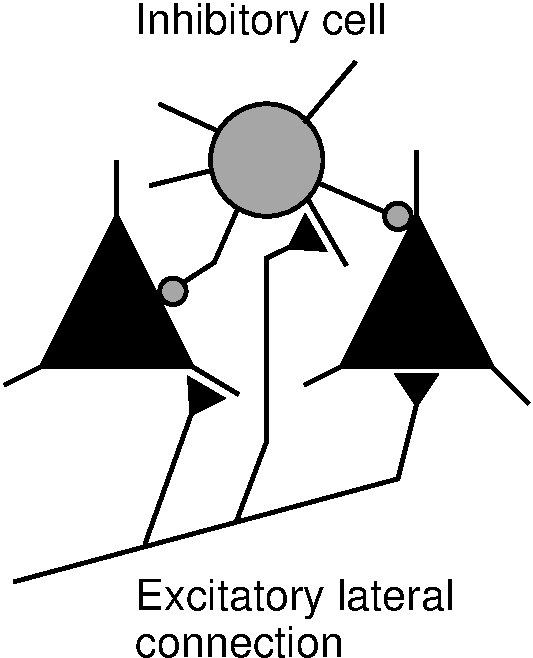
\includegraphics[width=0.25\textwidth]{weliky_microcircuit.pdf}
	\caption{Local microcircuit for long-range suppression through
          di- or poly-synaptic circuit in V1. Reproduced from
          \cite{Miikkulainen2005b} as adapted from \cite{Weliky1995}.}
	\label{V1MicroCircuit}
\end{figure}

More recent attempts at reconciling anatomy with function have been
able to further resolve some of the problem. In particular, there is
clear evidence showing that excitatory synapses onto excitatory and
inhibitory neurons differentially target their recipient
neurons. Excitatory connection onto inhibitory interneurons seem to
preferentially synapse perisomatically, in contrast with recurrent
long-range excitatory connections which have been shown to target
their recipient neurons dendritically
\citep{Gilbert1990,McGuire1991}. Additionally, at least a subset of
inhibitory interneurons seem to preferentially target the soma of
pyramidal and stellate cells they inhibit \citep{Markram2004}. On that
basis it is reasonable to assume that inhibitory connections are, in
general, stronger and may act divisively.

Although these divergent properties of excitatory and inhibitory
neurons were only discovered recently it had long been proposed that
inhibitory interneurons are inherently more effective at suppressing
activity than recurrent excitatory connections are at exciting the
network, but due to a high threshold or some other related mechanism
the inhibitory neurons are not strongly recruited unless there is
strong afferent input \citep{Sillito1979}, as would be the case under
high contrast conditions. Although it is now clear that network
effects allow for strong long-range inhibition through di- or
poly-synaptic connections under the right stimulus conditions, the
mechanisms by which contrast dependent behaviors emerge from the
cortical circuit are still only vaguely characterized.

A number of models have been developed to explain contrast dependence
of contextual effects on the basis of the general principle of
asymmetry between the response properties of excitatory and inhibitory
neurons. One of the first to publish such a model were
\cite{Stemmler1995}, who suggested inhibitory neurons require higher
external input rates before activating because they receive
significantly less spontaneous background input as compared to
excitatory neurons, an effect known as stochastic resonance. Although
this mechanism has at least been theoretically reaffirmed
\citep{Bezrukov1997}, there is no experimental data establishing it as
a functionally significant mechanism in V1. Other models, hoping to
account for a wider array of RF effects implement such a mechanism
directly by setting a higher threshold in the inhibitory population
and introducing very strong lateral excitation of inhibitory neurons
\citep{Schwabe2006}. Another suggestion was made by \cite{Somers1998},
who in addition to a simple threshold asymmetry, also point to the
claim by \cite{Thomson1994} and others \citep{Abbott1997,Tsodyks1997},
that synaptic depression causes recurrent excitation to quickly
decline in efficacy during high frequency stimulation, while
facilitation of excitatory synapses onto inhibitory interneurons
increases transmission efficacy as presynaptic firing rates increase
\citep{Thomson1995}. The suggestion that inhibitory neurons have a
higher contrast threshold has become very popular in the theoretical
literature of the past 20 years, however as of yet there is only
limited evidence to support this core assumption and there are a
number of alternative or concurrent mechanisms that may explain all or
at least some of the contrast dependent effects.

As the last paragraphs have shown, inhibition and in particular
surround inhibition are at the core of the major discussions on
contrast dependent effects and surround modulation and a more thorough
understanding of the spatial, temporal and functional dynamics of
surround inhibition is required.

\subsection{Surround Suppression: Feedforward or Feedback?}

The last section highlighted how little we still know about the origin
of surround suppression and inhibition. There is still significant
controversy whether surround suppression originates in feedforward or
feedback pathways or whether both contribute over different spatial
scales. This includes suggestions that surround suppression in the
classical RF are mediated through synaptic depression in the
thalamo-cortical afferents \citep{Carandini2002}, broadly tuned
inhibition by thalamo-cortical recipients, long-range excitation of
local inhibitory interneurons or even through various feedback
mechanisms. This section will detail the evidence for each of these
proposals, the possibly anatomical origin of each of these mechanisms
and tease apart the circuit by looking at interactions between
surround suppression, stimulus size and contrast.

Since the circuitry of the cortex is so complex, the task of
segregating feedforward and feedback contributions to surround
suppression is difficult. Although only a starting point, one
way of starting to tease these two possible contributions apart is to
look at the time course of suppression. In the literature early and
late components to surround suppression have been identified. The
early component is characterized as being driven by lower CRF
contrasts with spatio-temporally broad band tuning and little
adaptation \citep{Levitt1997,Cavanaugh2002a}. The late component on
the other hand is driven more strongly by high contrast stimuli in the
CRF, has sharp spatio-temporal tuning and can be strongly affected by
adaption \citep{Levitt1997}. Evidence suggests that the early, broadly
tuned component originates in the LGN and the thalamocortical
recipient layer of visual cortex \citep{Blasdel1984a,Hawken1996}. In
monkey cortex in particular, this broadly tuned suppressive effect is
only weakly evident in the LGN and is thought to arise much more
strongly in layer 4 of striate cortex \citep{Webb2005}, which may have
some correspondence to the broadly tuned inhibitory population
identified by \cite{Hirsch2003}. \cite{Carandini2002} on the other
hand suggest that there is a synaptic explanation for surround
suppression, primarily due to the speed with which the suppression
arrives, its immunity to cortical adaptation and the fact that it is
restricted to the CRF. However, they concede that synaptic depression
doesn't account for gain control and the abolishment of
cross-orientation suppression by GABA$^{A}$ blockade, so a mechanism
that can account for all these phenomena may still be preferable. In
that vein, \cite{Webb2005} propose two inhibitory mechanism one of
which sums local activity in a neurons CRF and divides the response of
the CRF and the later component that receives inputs from a much
larger area but provides narrowly tuned suppression. The broadly tuned
component in particular has a strong relationship with contrast gain
control, which has been firmly established to act
divisively. Independent work by \cite{Xing2005} supports the
suggestion of two inhibitory components and further expand on the size
dependence of these two components. Specifically, they conclude that
the tuned component is recruited far more strongly for larger stimuli,
which seems to confirm a contribution from beyond the CRF.

This recent work has identified two clear and distinct inhibitory
components but have not yet fully described which mechanisms and
circuits they are mediated by, the next section will attempt to
address this shortcoming.

\subsection{Distinct Inhibitory Populations}

In order to begin teasing apart the origin of intracortical surround
suppression mediated by local inhibitory circuits it is necessary to
consider the different candidate cell classes. While there are a long
list of different inhibitory cell types based on their morphology and
spiking behavior, recent techniques have divided inhibitory into
several broad, functionally distinct classes based on their
immunoreactivity. The two cell types considered here are parvalbumin
(Pv-ir) and somatostatin (Sst-ir) immunoreactive neurons, which are
primarily differentiated by the cellular locus of their synaptic
targets. While Pv-ir neurons seem to target pyramidal cells
perisomatically, Sst-ir neurons target their recipients
dendritically. The following subsections will detail the anatomical,
physiological and functional differences between these cell classes.

\subsubsection{Parvalbumin Immunoreactive cells}

The two main cell types, which exhibit parvalbumin immunoreactivity
are the chandelier and basket cells \citep{Binzegger2004}. While
chandelier cells make up only a small fraction of GABAergic neurons in
the cortex and are primarily found in layer 2/3, the fast-spiking (FS)
basket cells are the predominant interneuron subtype in the mammalian
cortex across all lamina, accounting for 42\% in layer 2/3 and layer 5
and 78\% in layer 4 of the cat \citep{Hogan1992,Huxlin2001} and up to
74\% across cortical layers in macaque \citep{VanBrederode1990}. The
abundance in the thalamocortical recipient layers and the fact that
they preferentially target the soma and proximal dendrites of spiny
neurons with multiple strong synapses, exhibiting high probability of
GABA release \citep{Freund2007,Markram2004}, ensures basket cells are
of tremendous interest. On that basis it has been suggested that the
perisomatic connectivity profile of basket cells gives them the
ability to provide shunting inhibition to layer 4 spiny neurons,
acting divisively to control their response gain \citep{Wilson2012}.

Basket cells can be further subdivided, primarily based on their size,
into clutch and large basket cells. However all basket cells can make
multiple connections onto a target pyramidal neuron
\citep{Somogyi1983} and have a considerable spatial extent
\citep{Kisvarday2002}. In particular, studies in cat area 17 and
macaque V1 have identified basket cells 1-2 mm in extent
\citep{Somogyi1983,Lund1987,Lund1991,Martin1983} and single cell
tracing studies have even identified large basket cells, which give
off a roughly uniform number of boutons across a large diameter
spanning up to two hypercolumns \citep{Buzas2001}. A schematic
representation of the basket cell connectivity profile is summarized
and compared against both the orientation column structure and the
excitatory connection profile in Figure
\ref{BasketCellExtent}. Functionally such a connectivity profile may
indicate that basket cells can suppress neurons with widely varying
orientation, which may implicate basket cells as an important
mechanism to sharpen orientation preference.

\begin{figure}
	\centering
        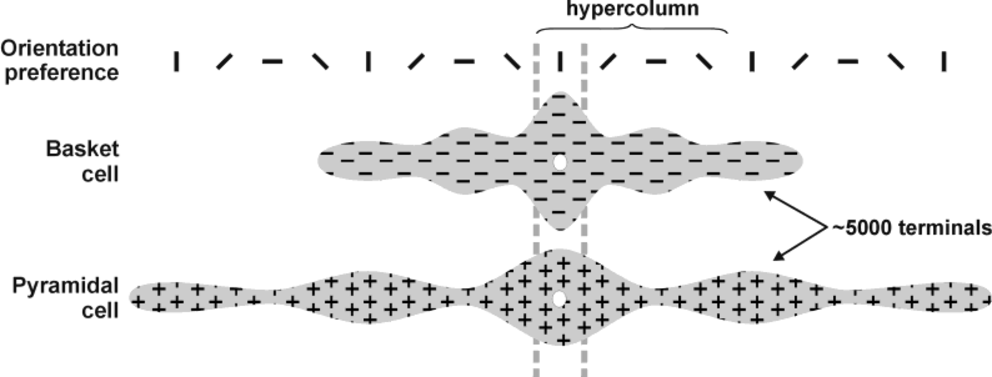
\includegraphics[width=1.0\textwidth]{basketcellextent.pdf}
	\caption{Summary schematic comparing relationship between
        long-range basket cell and excitatory connectivity with the
        underlying orientation preference structure. Upper legend
        represents different orientation domains in the cortical
        topographic map. Grey dotted lines indicate the orientation
        column within which soma of the simplified basket cell and
        excitatory neuron are found. The grey field with minus signs
        indicates the extent of inhibition provided by the basket cell
        connections considered in the current study. The grey region
        with plus signs indicates the excitatory field of a
        stereotypical pyramidal cell based on previous data by
        \cite{Bosking1997,Kisvarday1997a} and others. The height of
        the grey plus/minus regions indicates the number of axon
        terminals provided in that column. While basket cell terminals
        show local maxima every half hypercolumn distance, pyramidal
        cell terminals are maximal at every full hypercolumn
        distance. Reproduced from \cite{Buzas2001}.}
	\label{BasketCellExtent}
\end{figure}

In terms of their spiking behavior Pv-ir cells are characterized as
being fast fast-spiking (FS) neurons, often firing in bursts with a
very short response latency. Further, evidence from somatosensory
cortex in rodent and lagomorph species suggests they receive strong
input from thalamocortical afferents arriving in layer 4 and very
effectively suppress sustained firing from spiny neurons receiving
inputs from the thalamus \citep{Swadlow2003}, implicating them in
feedforward inhibition. This feedforward inhibition circuit is shown
in Figure \ref{burkhalterpv}. Their effectiveness in suppressing
feedforward activity can be explained by the large number of
thalamocortical axons they receive, which exhibit faster kinetics than
those targeting spiny neurons \citep{Cruikshank2007,Gabernet2005}, and
the fact that they evoke large inhibitory responses in spiny cells
\citep{Cruikshank2007,Gabernet2005}.

It is also important to note that the thalamocortical synapses onto
the Pv-ir population have been shown to be depressed by repetitive
activation, resulting in weaker feedforward inhibition at high
stimulation frequencies \citep{Gabernet2005}, a property which may
indicate lower activation of the PV population at high contrasts. The
Pv-ir population may also play an important role in network
homeostasis as activity blockade has been shown to decrease the
efficacy of Pv-ir inhibition \citep{Bartley2008}, thereby indirectly
up-regulating activity in excitatory cells. Further, selectively
up-regulating Pv-ir cells using optogenetic stimulation was shown to
have a similar effect as lowering the contrast, which is to increase
preferred size and weakening surround suppression
\citep{Nienborg2013}. This is compatible with the idea that Pv-ir
neurons provide strong feedforward inhibition such that the input
drive in the cortex is decreased, as would be observed under low
contrast conditions. Overall then, Pv-ir neurons show strong
interaction with stimulus contrast and may be involved in regulating
the gain of the network with complex implications for the contrast
response of the network.

\begin{figure}
	\centering
        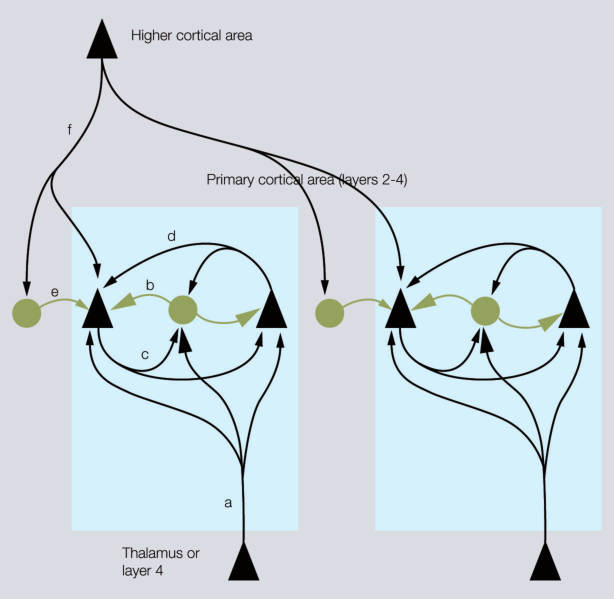
\includegraphics[width=1.0\textwidth]{burkhalter_pv.pdf}
	\caption{Inhibitory networks involving fast-spiking
        parvalbumin-immunoreactive neurons in thalamocortical,
        interlaminar and interareal cortical circuits. Feedforward
        excitatory thalamocortical inputs to pyramidal cells, spiny
        stellate neurons ($\blacktriangle$) and fast spiking
        interneurons ($\newmoon$) in layers 2-4 (a). Inputs to
        interneurons are stronger (large arrowheads) than inputs to
        spiny cells. PV neurons provide strong (large rectangular
        endings) feedforward inhibition (b) to spiny cells. Feedback
        inhibition (c) results from PV neurons that are excited by the
        same spiny neurons that they inhibit. These reciprocally
        connected spiny neuron/PV neuron pairs share common inputs
        (e.g., cells in layer 4 from thalamus or cells in layer 2/3
        from layer 4) creating recurrent excitatory (d) and inhibitory
        subnetworks (contained within blue shaded boxes). ‘Lateral’
        inhibition (e) of these subnetworks results from PV neurons
        that are driven by excitatory feedback connections (f) from
        outside the subnetworks (e.g., by layer 5 to layer 2/3
        connections or feedback from higher cortical areas). Notice
        that ‘lateral’ inhibition is weaker (small rectangular
        endings) than feedforward and feedback inhibition and impinges
        on multiple subnetworks. Reproduced from
        \cite{Burkhalter2008}.}
	\label{burkhalterpv}
\end{figure}

There is still considerable debate on the extent to which this
subpopulation is tuned to a particular orientation. Most
visuo-cortical models employ broad, non-specific GABAergic inhibition
\citep{Somers1998,Troyer1998}. This seems to be supported by
anatomical evidence, which has long shown that inhibitory projections
are generally diffuse and display low specificity for specific
stimulus features \citep{Albus1994,Kisvarday1997a}. Further,
electrophysiological data paints a similar picture, revealing
suppression that is broadly tuned for stimulus attributes, providing
orientation unspecific suppression from a visual region that is
coextensive with the classical RF \citep{DeAngelis1992}. Recent
attempts at studying the Pv-ir neurons at the single neuron level have
revealed a mixed picture. While the cells as a whole were broadly
tuned to various stimulus features, individual branches often
displayed very high specificity, which may underlie subfield
antagonism and contribute to a push-pull configuration
\citep{Kisvarday2002}. Studies in mouse visual cortex seem to confirm
such a dual purpose of Pv-ir neurons, although they also find higher
heterogeneity in the Pv-ir population \citep{Runyan2010}. This may
indicate a laminar differentiation in function as studies of Pv-ir
neurons in the thalamocortical recipient layer 4 have characterized
them to exhibit very broad tuning, due to their low spiking threshold
and more convergent inputs \citep{Ma2011}. However, even in layer 2/3
most Pv-ir cells displayed broad orientation tuning
\citep{Hofer2011}. Further studies in cat area 17 find very similar
results identifying a class of inhibitory complex cells in layer 4
exhibiting weak orientation tuning \citep{Hirsch2003}, which can
primarily be accounted for by the tuning of synaptic responses and a
lower spike threshold \citep{Nowak2008}. A more recent study in
auditory cortex seems to affirm these conclusions, hypothesizing that
`while PV neurons may provide broadly tuned feedforward inhibition for
a rapid control of ascending inputs to excitatory neurons, the delayed
and more selective inhibition from SOM neurons may provide a specific
modulation of feedback inputs on their distal dendrites`
\citep{Li2014}. Further study will be needed to confirm whether these
results extend to the primate, however it is clear that basket cells
generally display weaker tuning than spiny neurons in V1.

Based on our current knowledge of Pv-ir cell population and more
specifically the basket cells, it is clear that they provide a good
candidate mechanism to account for a number of phenomena. Their fast
response profile, large spatial extent and the relative weakness in
their orientation tuning may allow them to carry out fast, adaptive
gain control, broadly tuned suppression and thereby sharpen the
orientation preference of the PNs in their vicinity. So while synaptic
depression may still provide an alternative explanation for many of
these phenomena, it is likely that the Pv-ir population carries out at
least some of these functions.

\subsubsection{Somatostatin Immunoreactive cells}

The Sst-ir population has been characterized to a lesser extent, but a
general consensus is beginning to emerge around their function and
electrophysiological properties. The Sst-ir cells account for around
half of the non-PV-expressing neurons \citep{Gonchar2007,Xu2010} and
preferentially synapse onto distal dendrites and dendritic tufts of
pyramidal neurons \citep{DiCristo2004,Silberberg2007}, on the basis of
which it has been suggested that Sst-ir neurons act subtractively
\citep{Wilson2012}.

In trying to characterize the excitatory inputs to Sst-ir cells in
layer 2/3 of the mouse, \cite{Xu2009} determined that unlike Pv-irs,
the main source of excitation of Sst-irs were horizontal axons within
layer 2/3 not the ascending layer 4 axons. This property also
contributed to the size dependent responses of the Sst-irs, which were
shown to be recruited progressively more strongly when they were
exposed to optogenetic photostimulation of increasing
diameter. Importantly, the Sst-ir response grew larger even when
photostimulation reached beyond its maximal dendritic extent,
demonstrating that the recruitment of increasingly more distant
pyramidal cells provided their main excitatory drive. This putative
circuit is shown in Figure \ref{som}, exhibiting their pooling of
tuned, excitatory input from pyramidal cells across a large area,
providing only very local inhibition. Additionally it seems that
Sst-ir interneurons are capable of disinhibiting the thalamocortical
recipient layer 4 by targeting Pv-ir cells \citep{Xu2013}.

In terms of their response properties the Sst-ir neurons have been
shown to exhibit much lower levels of spontaneous and evoked activity,
stronger orientation and direction selectivity and longer response
latencies than Pv-ir neurons in mouse visual cortex
\citep{Ma2011}. These properties are consistent across both layer 2/3
and 4 and may point to a role in gating later arriving intracortical
excitatory inputs. In terms of their tuning properties Sst-ir neurons
display smaller On/Off subfields with less overlap than nearby spiny
neurons and orientation tuning on par with pyramidal neurons. While
most data on their tuning properties comes from rodent visual cortex,
which does not exhibit a topographic organization of orientation
tuning, it seems the stronger orientation selectivity of Sst-ir cells
can be accounted for by their preferential connectivity to neurons
with similar orientation preference as well as a higher spiking
threshold and weaker excitatory inputs \citep{Bartley2008}. Another
interesting feature of Sst-ir response properties is the fact that
although their excitatory inputs are weak, they are facilitating
resulting in delayed but strong activation under high frequency
stimulation \citep{Beierlein2003,Bartley2008,Tan2008}. Based on these
properties, Sst-ir neurons would only be recruited to provide
significant inhibition if the stimulus contrast or size reaches a
certain level \citep{Adesnik2012}. Thus they could provide a direct
mechanism for contrast dependent size tuning and surround modulation
effects, being only weakly recruited when contrast or stimulus size is
low but becoming strongly activated at higher contrast levels and for
larger stimulus sizes.

% Comment on difference between high threshold and Sst-ir cell hypothesis

Another suggested role for Sst-ir neurons is the gating of feedback
signals on the distal dendrites of principal neurons. The Martinotti
cells, which provide strong axonal projections to layer 1 of the
cortex, make up a large proportion of Sst-ir neurons in layer 2/3 of
the cortex and are therefore well placed to suppress feedback signals
arriving in the superficial layers of the cortex
\citep{Fanselow2008,Gentet2012}. In the rodent somatosensory cortex,
\cite{Gentet2012} showed that Sst-irs in layer 2/3 become
spontaneously active during passive wakefulness but are strongly
suppressed during active whisking behavior, presumably by the
vasoactive intestinal peptide (Vip)-ir population. The Sst-ir cells
may therefore be involved in mediating top-down control of sensory
processing, effectively gating context-dependent processing in a state
dependent manner.

\begin{figure}
	\centering
        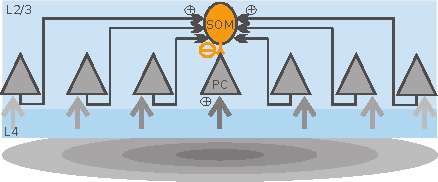
\includegraphics[width=1.0\textwidth]{adesnik_som.pdf}
	\caption{Schematic illustration of the cortical circuit in
          layer 2/3 contributing to surround suppression. As a visual
          stimulus expands (larger stimuli are shown in lighter grey),
          recruitment of adjacent PCs increases Sst-ir excitation
          through horizontal axons (horizontal arrows). Reproduced
          from \cite{Adesnik2012}.}
	\label{som}
\end{figure}

In summary, Sst-ir neurons seem to provide delayed and
feature-selective feedback inhibition, which puts them in a good
position to effectively gate late arriving intracortical excitatory
inputs arriving from either lateral or feedback connections but may
also be implicated in suppressing feedforward inhibition by
inactivating layer 4 Pv-ir cells.

\subsubsection{Vasointestinal peptide expressing interneurons}

The previous review focused primarily on the two most common types of
inhibitory interneurons, the Parvalbumin (PV) and
Somatostatin-expressing (Sst) cells, since then a number of studies
have focused on the role of 5HT3ar-expressing interneurons and
particularly the vasointestinal peptide (Vip)-expressing subgroup
\citep{Fu2014, Higley2014, Kepecs2014, Lee2013}.

The Vip subgroup is particularly concentrated in upper, associative
layers and feedback layers of the cortex, as shown in figure
\ref{GABADistribution} by \cite{Rudy2011}. The most striking finding
was their central role in state dependent modulation during active
whisking tasks. \cite{Lee2013} found that S1-projecting vM1 pyramidal
neurons strongly recruited Vip-expressing interneurons in superficial
layers of somatosensory barrel cortex, which in turn inhibited
somatostatin-expressing interneurons causing effective disinhibition
of cortical pyramidal cells. These results could were then affirmed
through optogenetic stimulation of Vip neurons in mouse V1,
artificially mimicking the effects locomotion \citep{Fu2014}. When
considered in conjunction with previous studies that established
strong cholinergic and nicotinic inputs to Vip neurons from the basal
forebrain \citep{Wickersham2009}, this suggests a strong involvement
of Vip neurons in a cortical circuit responsible for the enhancement
of activity in sensory cortex by behavioural state.

\begin{figure}
	\centering
        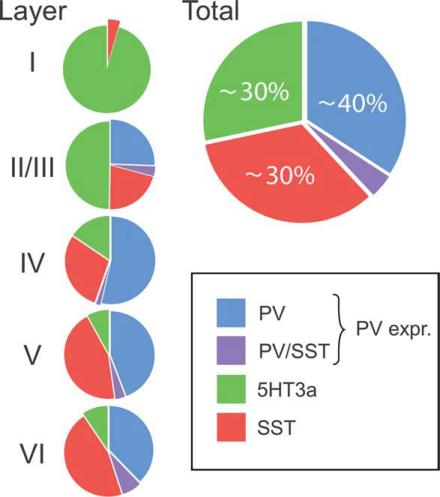
\includegraphics[width=0.4\textwidth]{GABADistribution.pdf}
	\caption{Distribution of GABAergic interneurons in S1
        cortex by immunohistological marker. Reproduced from
        \cite{Rudy2011}.}
	\label{GABADistribution}
\end{figure}


\subsubsection{Connectivity between different cell types}

In order to gain an understanding of the circuits the different
interneuron cell types are involved in, it is important to consider
their interconnectivity. Several studies have sought to determine the
connectivity between Pv-ir, Sst-ir and other interneuron types. The
core findings of these studies determined that Pv-ir cells
preferentially inhibit one another, Sst-expressing cells avoid one
another and inhibit all other types of interneurons particularly the
Pv-ir cells \citep{Xu2013}, while a third type, the Vip-ir cells
preferentially inhibit Sst-ir cells \citep{Pfeffer2013}. This
connectivity profile is schematically represented in Figure
\ref{gaba_circuit}. In mouse cortex the Pv-ir, Sst-ir and Vip-ir cells
accounted for about 40\%, 18\% and 8\% of the GABAergic population,
respectively \citep{Xu2010}, and although these percentages vary
considerably across species Pv-ir and Sst-ir are always the two most
commonly expressed GABAergic populations.

\begin{figure}
	\centering
        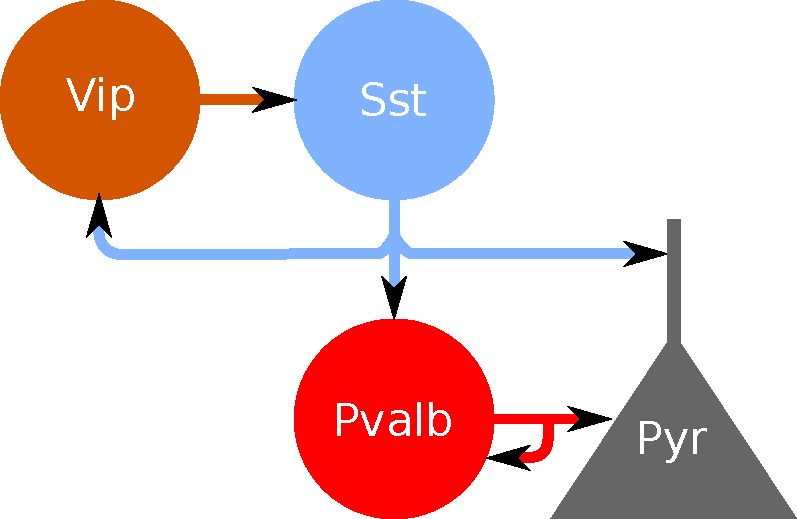
\includegraphics[width=0.7\textwidth]{pfeffer_gabacircuit.pdf}
	\caption{Connectivity between somatostatin (Sst),
        parvalbumin (Pv), vasoactive intestinal peptide (Vip)
        expressing and pyramidal (Pyr) cell types. Adapted from
        \cite{Pfeffer2013}.}
	\label{gaba_circuit}
\end{figure}

Recent tracing techniques have also been able to establish that
excitatory cells provide orientation specific inputs to the inhibitory
population. Using viral tracing techniques \cite{Liu2013} are able to
trace inputs to inhibitory and excitatory neurons in the cat visual
cortex.

\section{GABAergic regulation of plasticity and column structure}

Experience dependent plasticity has been shown to shape the
organization of the sensory cortex during the critical period and
beyond. Dark rearing \citep{Fregnac1978} and monocular deprivation
(MD) experiments \citep{Shatz1978} in particular have confirmed the
fundamental importance of sensory experience in shaping the
development of the cortex. The mechanisms controlling the onset of the
critical period and regulation of plasticity thereafter have also been
studied extensively and a large body of evidence points to the
important role of the inhibitory neurotransmitter
$\gamma$-aminobutyric acid (GABA) in regulating synaptic
plasticity. However as the above paragraphs have shown the population
of GABAergic neurons is highly heterogeneous with hugely divergent
anatomical and functional profiles. Using specific pharmacological and
genetic populations it has been possible to narrow down the
involvement of certain interneuron subtypes in shaping critical period
plasticity and column structure in the cortex.

One of the first indications that GABAergic circuits are involved in
shaping plasticity came when it was shown that a gene-targeted
disruption of the GABA synthetic enzyme glutamic acid decarboxylase 65
(GAD65) could delay critical period onset indefinitely
\citep{Fagiolini2000}. In order to further narrow down the specific
GABA circuits underlying visual cortical plasticity, more specific
pharmacological manipulations were required. On that basis
\cite{Fagiolini2004} used benzodiazepine infusions, known to
selectively enhance GABA type A ($GABA_A$) receptor-mediated currents
through the $\alpha1$ subunit \citep{Rudolph1999}, in conjunction with
MD to prematurely trigger ocular dominance plasticity in mice. These
$GABA_A$ receptor-$\alpha1$ subunits are preferentially enriched at
somatic synapses receiving input from Pv-ir large basket cell
terminals \citep{Klausberger2002}, strongly implicating large basket
cells in visual cortical plasticity.

Beyond controlling the timing of critical period plasticity further
experiments using benzodiazepines have shown strong effects on the
columnar organization of the cortex. The experiment by
\cite{Hensch2004} locally infused regions of cat area 17 with the
$GABA_A$ agonist diazepam and an inverse agonist (DMCM) and studied
the effects on the ocular dominance columns. Chronic treatment with
diazepam had little effect in the functional properties of mature
cortical neurons in vivo apart from enhancing inhibitory postsynaptic
currents. However, the treated hemisphere exhibited reduced
binocularity of single unit responses and wider OD columns near the
infusion site. Infusion with the benzodiazepine inverse agonist DMCM
had the inverse effect, resulting in less discrete and narrower
columns near the infusion site. These results suggest that the
diazepam mediated enhancement in competition reduces binocularity of
single-unit responses, as well as sharpening and widening the
anatomical segregation of monocular regions near the infusion
site. This once again suggests that $GABA_A$ inhibitory currents,
primarily originating from Pv-ir neurons in the cortex, are
fundamentally important to shaping the plasticity and organization of
the cortex.

In order to establish how ocular dominance plasticity emerges during
monocular deprivation, \cite{Kuhlman2013} developed even more
precisely targeted pharmacological manipulations. By selectively
expressing specific receptors on Pv-ir cells they were able to
selectively up- and down-regulate their activity. Their results
indicate that a rapid, but transient reduction in Pv-ir cell firing
restores pyramidal cell firing to pre-deprivation levels allowing
competitive plasticity to occur. Pv-ir neurons therefore seem to play
a permissive role in visual cortical plasticity. Interestingly adult
sensory plasticity such as reinforced associative learning occurs
through a similar mechanism, where cholinergic activation of layer 1
interneurons suppresses Pv-ir neural activity allowing associative
fear learning to occur \citep{Letzkus2011}. All this work suggests a
crucial role for Pv-ir neurons in controlling cortical plasticity
during the critical period and beyond.

\section{Functional Roles of Intracortical Connectivity}

A major feature of the neural code in the cortex is the elimination of
redundancy in order to achieve a sparse representation of the input or
if there is insufficient information to fill in the missing
information based on remembered statistics of the visual world. Sparse
coding in developmental models of the primary visual cortex can be
achieved by allowing lateral inhibitory connections to develop
non-isotropic connectivity, which allows the network to learn the
redundant features of the input and suppress them. If such development
is not allowed to take place and isotropic surround suppression is
employed, cross-orientation stimuli, belonging to a separate object or
contour may be suppressed, thus reducing the information content
encoded by the network. Therefore long-range isotropic suppression has
to be considered destructive \citep{Miikkulainen2005b}. Similarly,
strong lateral excitation will activate neural ensembles representing
non-existing inputs based solely on previous input statistics. While
this is desirable when very little information is available it can
disrupt sparse code formation by expanding the activity bubble or
causing the false detection of a stimulus. Therefore the sensory
cortex has to maintain a fine balance not only between excitation and
inhibition but also in combining past information with the feedforward
information stream arriving in the cortex. Identifying and modeling
the circuits involved in these processes is a fundamental challenge
for neuroscience and will hugely contribute to extending our
understanding of cortical information processing.

Over the last decade evidence for multiple separate inhibitory
populations, subserving different functions, has been considerably
strengthened. Although their precise properties in regard to
morphological and electrophysiological heterogeneity are still unclear
there are a number of identifiable circuit elements. Afferent input
provides strong, low latency excitation to the Pv-ir neurons in the
thalamocortical recipient layer 4, which in turn act as both a
feedforward inhibition and dynamic gain control mechanism on the
broadly activated excitatory cell population. This results in local
decorrelation of the neural activity, which allows recurrent
excitation to amplify the activity in the local neural
ensemble. Meanwhile Sst-ir neurons begin to integrate the local
activity through the local and long-range orientation-specific lateral
connections. If their inputs are sufficiently strong they will
activate allowing this polysynaptic circuit to reduce long range
correlation in the input activity, further reducing redundancy. If
they are only weakly activated on the other hand, long-range lateral
excitatory connections aren't outcompeted and the circuit can fill in
weak or missing information based on past statistics. Under such
regimen the differential recruitment of the two separate inhibitory
populations would be responsible for a shift in cortical state from a
mode of redundancy-reduction and feature discrimination to one of
visual inference. Additionally, modulatory inputs to the cortex like
cholinergic modulation arriving from the nucleus basalis may mediate a
number of effects, whether that is a shift in the circuit from a
down-state, where information is recurrently processed, to a
feedforward heavy up-state, by reducing feedforward inhibition and
boosting feedforward excitation, or a mode in which task-relevant
information is selectively filtered, is still unclear. The following
sections will outline how these possibilities have begun to be
explored by constructing a model based on the available experimental
evidence and will outline plans to begin testing some of these
different hypothesis.

\section{Contextual Modulation and Attention}

The computational task in vision is to map visual experience to the
cortical representation of that particular stimulus or if no such
representation exists, to extract lower level features in order to
encode them for future reference. Using this statistical model the
brain is then able to decide, which visual features carry behavioral
importance and which can be safely ignored. As such the neocortex has
to combine prior information with the incoming information stream and
quickly and reliably identify the most salient stimuli. It has often
been argued that this process is mediated by bottom-up and top-down
processes, although it seems likely that there is close coupling
between the two. This section will outline high level models of
attentional modulation, attempts to understand the neurobiological
processes behind them and more basic contextual modulation phenomena
may underly many of these higher level effects.


\subsection{Contextual and Attentional Phenomena in V1}

A number of phenomena associated with attention and contextual
modulation, including iso-orientation suppression or facilitation,
boundary detection, contour completion and noise exclusion have been
observed in V1. Although these phenomena are generally associated with
bottom-up attention they lay the foundation for higher level phenomena
such as pop-out and figure-ground segregation and may reveal more
about general mechanisms applying also to higher visual areas.

Basic contextual effects such as iso-orientation suppression have
already been discussed and models have begun to suggest the functional
connectivity mediating implicating both lateral and feedback
connections. While, \cite{Li2002} has proposed that pre-attentive
bottom-up processes allow V1 to generate a saliency map of the visual
input. However, the fact that higher cortical areas have also been
associated with saliency signaling and the lack of long range
intra-areal connectivity in V1 suggest that while it can encode local
saliency, feedback is required to globally integrate saliency across
visual space.

Feedback modulation of V1 activity has been implicated in a number of
effects, spatial attention being chief among them. Spatial attention
is thought to be able to select multiple low and high level objects in
the visual space across V1 and higher visual areas
\citep{McMains2004}. It is thought to underly noise exclusion,
observed by \cite{Dosher2000} and may be explained by effects similar
what has been experimentally observed during ionphoretic application
of ACh. Other effects that have been commonly been associated with
feedback in some form are the signaling of illusory contours, which
have been shown to be negatively signaled or deemphasized in V1
\citep{Ramsden2001} and boundary detection \citep{Poort2012}.  In the
planning section, concrete proposals will be made suggesting what
mechanisms may account for these phenomena and how they can be
implemented.

\section{Natural Image Statistics, Sparsity and Horizontal Connections}

It has long been hypothesized that connectivity in the cortex captures
the statistics of the sensory input in order to perform predictions
and maintain sparse representations of novel inputs
\citep{Simoncelli2001}. A wide range of work has explored the role of
the distributions of light intensities, color statistics and spatial
correlations in natural images. In particular, the power law
distribution of spatial frequencies in natural images has been widely
discussed in the literature but ultimately this largely seems to
reflect the scale invariance within natural images
\citep{Ruderman1997}.

Numerous studies and models have since been devised to address whether
the visual system takes advantage of the correlational structure of
natural images. These types of normative models were able to show that
surround inhibition, whether subtractive or divisive, could cancel out
correlations effectively whitening or decorrelating the activity in
the visual system \citep{Srinivasan1982, Atick1992}. In doing so they
quickly found that simple decorrelation wasn't sufficient to optimally
represent natural images because whitening does not eliminate all
structure in a natural image, e.g. edges and lines remain. By
introducing an explicit sparsity constraint, \cite{Olshausen1996} were
able to develop V1-like simple cell receptive fields with varying
orientations, spatial frequencies and sizes. These models indicated
that sensory system was optimizing two constraints, sparsity and
statistical independence. However, even these approaches cannot
achieve complete statistical independence since there are higher order
correlations even between non-overlapping receptive fields.

By introducing divisive normalization, \cite{Schwartz2001a} were able
to show that these types of dependencies could be further
eliminated. Furthermore, the weights used in the computation of the
normalization signal could be specifically optimized to maximize the
independence of the normalized responses. Additionally, they
demonstrated that the optimal weights were at least partly due to the
prevalence of extended contours in natural images. Attempting to
quantify the co-occurence statistics of contours in natural images,
\cite{Geisler2001} demonstrated that the performance in contour
detection tasks could be predicted by a local grouping rule derived
from the co-occurence statistics. The first explicit link to
horizontal connectivity was made by \cite{Sigman2001}, who noted that
the pattern of long-range patchy connectivity in the primary visual
cortex, linking iso-orientation columns has a close corespondence with
the observation of co-circularity in natural image statistics. Noting
the processes of iso-orientation suppression and contour integration,
they argue that iso-orientation suppression may serve to further
reduce redundancies in neural coding, thereby achieving greater
statistical independence, which would explain why neural responses
appear most sparse when presented with natural stimuli. Secondly,
observing that visual cortex can also exhibit colinear faciliation
under low contrast conditions \citep{Sceniak1999, Kapadia1999}, they
suggest that under low signal-to-noise conditions the cortex may act
to enhance repeated statistics to aid the identification of contours
and form.

These theoretical studies have hugely advanced our thinking about the
computations performed by the early visual cortex, however very little
work has been done to look at the actual structure of horizontal
connectivity in V1, largely due to the difficulty in obtaining data
from more than just a few cells. Even on the question whether
horizontal connections are anisotropic along the axis of preferred
orientation of the neuron, as would be expected from theoretical
studies, there is conflicting evidence. The result has been confirmed
in monkey \citep{Sincich2001}, tree shrew \citep{Bosking1997} and cat
\citep{Schmidt1997}, but conflicting results exist in macaque
\cite{Angelucci2002}. By performing analyses on an old tree shrew
dataset \cite{Hunt2011} investigated whether horizontal connections
captured the co-circularity of natural image statistics. Although they
found neurons, which exhibited co-circularity and anti-cocircularity
and hypothesize a role for both, given the small number of lateral
connections fields and the fact that second order properties are
highly sensitive to even small errors in the data, it is unclear how
strong this result is. Further research in this area is desperately
needed.
 %
%!TEX root = ../PhDthesis.tex
\chapter{Reproducible science and visualization}

Although the subject of this thesis is centered around modeling of the
visual cortex, a reproducible workflow is crucial to all scientific
disciplines and especially so in the computational sciences. As part
of the work presented in this thesis, we describe a new workflow to
make the exploration, analysis and publication of complex models
easier and more reproducible at every step. In particular this chapter
describes how the HoloViews library developed to aid the work as part
of the PhD achieves these goals and provides a general solution to
data visualization, storage and analysis that is now used in a number
of research projects. Every result in this thesis was generated using
this workflow and a fully reproducible record of the work is available
at \url{thesis.philippjfr.com}.

Developing such a workflow was essential to allow quick exploration of
the highly non-linear models developed as part of this
research. Specifically, when dealing with complex models with a large
number of parameters, which also evolve over time, existing tools were
not suited for the job. This is because a major component of this work
and work in other fields is an iterative process exploring some
parameter space, gaining insight into the behavior of the model and
then refining the model with the insights gained by careful
analysis. For this purpose we present a workflow, starting with the
declaration of a parameter space to explore, demonstrating how the
simulations can easily be launched locally or on a distributed cluster
and then be collected together for analysis. Finally we demonstrate
how the HoloViews library let's you load the data as it is generated,
monitor the progress and then provides powerful tools to visualize and
analyze the resulting data up to and including publication quality
figures.

We will begin by outlining the overall workflow and the philosophy
behind the individual components, before providing a case study on
the usage of the workflow as employed in this thesis.

\section{HoloViews: Building Complex Visualizations Easily for Reproducible Science}

One of the major contributions developed as part of this thesis is
development of the HoloViews data analysis and visualization library.
The library was developed to support this research in collaboration
with Jean-Luc Stevens and was published by Jean-Luc Stevens and myself
as joint first authors in the SciPy Conference Proceedings
\citep{Stevens2015}. Since then the library has become a popular
open-source library used in a wide range of scientific
disciplines. This section will outline the core design principles
behind HoloViews before applying it to a case study taken from one of
the results sections.

\subsection{Motivation}

In modern data analysis in scientific and engineering fields there is
often significantly more data available than a researcher can easily
review using standard plotting tools, in particular when the data is
dependent on a large number of variables, which cannot easily be
represented by the standard 2D or 3D plot types. The other barrier to
exploring these kind of datasets is that most plotting libraries are
not very well suited towards interactive analysis. The process of
visualizing is usually one that requires a lot of back and forth
between writing custom plotting code, viewing the results and then
customizing the plot or writing more plotting code to view the data in
a different way. All this back and forth between the code and what the
researcher actually wants to do, which is to view the data, can kill
productivity and is a major obstacle in analyzing complex
datasets. Furthermore, it results in a disjointed, inefficient
workflow, accumulating custom code, which has to be maintained and
often becomes unreproducible.

HoloViews solves these fundamental problems by making the data
immediately visualizable. Unlike standard plotting approaches the data
is always available on HoloViews objects so a plot does not become a
dead end, each piece of data is annotated with the appropriate
metadata so it can be composed and processed into further
plots. Further, HoloViews objects can easily be converted between each
other allowing very quickly iterating over different
visualizations. Finally HoloViews makes interactivity central to the
workflow, data with higher-dimensionality than can be meaningfully
represented on a simple plot can be explored through interactive
sliders or by laying the data out in complex, faceted plots.

HoloViews also improves the reproducibility of the results because
dependency on external plotting code is massively reduced, the
metadata is tightly coupled with the actual data and HoloViews'
declarative style provides a readable description of what exactly is
being plotted. Next we will highlight the core design principles of
HoloViews that makes it so powerful as a tool for analysis,
visualization and publication.

\subsection{Design Principles}

The overriding design principle of HoloViews that the user should not
have to write a complex recipe of how they want their data to be
displayed, instead HoloViews provides a set of declarative
datastructures, which allow annotating the data with a minimal amount
of metadata to display a visual representation automatically and
transparently - the data should simply reveal itself.

The second core principle of HoloViews is that there should be a very
clear distinction between the details of visualization and actual data
and metadata required to describe a dataset. This means that the
atomic data objects (or Elements) should be very lightweight wrappers
around the actual datastructure along with a small amount of semantic
metadata. This allows creating, working with and storing the data
independent of the plotting code or any concerns about the visual
aesthetics of the plots.

The third design goal is the composability of the Elements. By
ensuring that different components can easily be composed together it
becomes very easy to build even complex plot types from simple
components. HoloViews provides operators and methods to make
overlaying and composing plots in layouts and grids very
straightforward.

These three guiding philosophies make HoloViews into an extremely
powerful tool to explore complex datasets easily while also providing
the flexibility to generate publication quality figures. In the next
section we will outline how this fits into an overall workflow and
demonstrate what these principles mean in practice. For a more in
depth review of the philosophy and principles behind the library refer
to the HoloViews paper in Appendix \ref{SciPyPaper}.

% Insert reference to HoloViews paper and to the appendix

\section{A unified workflow for the analysis of complex computational models}

When working with complex computational models or analyses it is often
necessary to launch large scale, parallel parameter explorations,
gather the results and apply analyses to the results. This often
involves separate scripts to launch the simulations and analysis
either locally and on a cluster and separate tools to gather this data
up from a shared storage location to visualize the results or apply
further analyses. This often results in collections of different
scripts and data files, which stitch together a disjointed workflow,
providing a serious barrier to reproducibility. As an alternative we
developed an integrated workflow based on the Lancet and HoloViews
libraries, which let's you trivially launch parameter explorations
either locally or on a cluster, monitor the progress and then lazily
load just the required subset of data for further analysis.

Through a concrete example we'll explore how to specify each stage in
this analysis pipeline, highlighting the ease with which we can
launch, analyze and revise a model using this system. For this purpose
we'll use a parameter exploration that is part of one of the results
chapters, skipping over the evaluation of the actual results for the
time being. While this is just one example, all the results produced
as part of this thesis are made available in the same format to
provide a fully reproducible record of the work done as part of this
project.

\subsection{The Jupyter notebook environment}

In order to generate truly reproducible research it is not enough
simply to make sure that the analysis code is re-runnable but rather
guiding someone who is trying to reproduce the results through each
step so that they can not replicate the results but also understand
each step so that they can begin modifying the workflow to take the
research further. This is the distinction between mere replicability
and true reproducibility. In the past this required documenting the
code and results meticulously in separate files but even then this
workflow usually devolves into chaining script after script until the
workflow becomes difficult or impossible to follow for an external
researcher. The Jupyter notebook environment, spawned through the
IPython project \citep{Perez2007}, promises a solution to this problem
by providing a platform that allows interleaving code with rich media
output and exposition, providing a detailed account of the steps
required to generate results and figures in a publication.

The entire workflow presented here is centered around the Jupyter
notebook, while not depending on it. It is what allows us to specify
an experiment to run, monitor progress and present the results, all
accompanied by detailed exposition describing each stage. Each chapter
of this thesis will therefore be accompanied by one or more Jupyter
notebooks, which provide a fully reproducible account of how each
figure was generated along with supplemental materials and results.

\subsection{Step 1: Specifying a parameter space}

The usual process of launching a parameter space analyses is to write
scripts to launch the jobs either locally or on a remote cluster. The
resulting files then have to be gathered up appropriately and should
preferably be accompanied by a log of the precise environment used to
launch the jobs. Lancet makes it trivial to specify jobs to execute
and will handle launching these jobs both locally and on a cluster,
keeping track of the files that were generated, the environment used
and any other extraneous information like version control data. In
\cite{Stevens2013a} the fundamental ideas behind Lancet are outlined
in detail so here we will focus on how it integrates with the overall
workflow outlined in this chapter.

In this outline of the workflow we will be working with one of the
models that will be explored and developed as part of this thesis. To
get a better understanding of the model we want to vary multiple
parameters, apply measurements and analysis to the model and then
evaluate the results. Defining the parameter space to explore is
incredibly straightforward. First we declare constant parameters, in
this case just the ``area`` of the model and the times in the
development of the model at which we want to apply measurements to the
model. Secondly we declare the varying parameters, in this case we
simply combine a ``Range`` of lateral excitatory strength
(``latexc\_strength``) with another ``Range`` of contrasts. The
multiplication operator automatically expands this parameter space by
taking the Cartesian product of the two varying sets of
parameters. Finally we combine the constant and varying parameters
into the overall parameter set for the batched experiment.

\begin{minipage}{\linewidth}
\begin{lstlisting}
times = [1000*i for i in range(21)]
constants = lancet.Args(area=3.0)
parameter_space = lancet.Range('latexc_strength', 0, 3.0, 11) * lancet.Range('contrast', 10, 100, 10)
batch_arguments =  constants * parameter_space * lancet.Args(times=times)
\end{lstlisting}
\end{minipage}

\subsection{Step 2: Specifying analysis}

Having defined the parameter space the next step is defining the
actual model to run and any measurements or analysis that are applied
to it. In this example we are working with the Topographica neural
simulator, which allows training large scale rate-based models on
visual input patterns. Here we load the SCAL model, which we will
present in the next chapter and define a measurement of the
orientation map with subsequent applied to the measured orientation
maps. These tasks will now be measured for each of the parameters
defined above, at each of the declared times. This makes it incredibly
easy to set up deferred execution of any number of measurements and
analyses and even allows setting up complex chains of measurements and
analysis by declaring the output of one analysis as input to the next.

The ``Collector`` object will then apply the measurements at the times
defined as part of the parameter space, storing them as small
individual files, which can be loaded independently or all
together. Another benefit is that the Collector automatically records
the precise measurements that were defined ensuring that the results
stay reproducible. Since the results are stored inside HoloViews
objects they are instantly visualizable. All of these features ensure
that with very minimal effort by the user all the specifications to
set up the experiment are recorded, the results can easily be accessed
and the entire process can easily be replicated from the logs that are
output by Lancet.


\begin{minipage}{\linewidth}
\begin{lstlisting}
  c = Collector()

  # Measurement
  c.collect(measure_or_pref, frequencies=[1.4, 1.6, 1.8])

  # Analysis
  c.Pinwheels.V1   = c.analyze(c.ref.OrientationPreference.V1 *\
                     c.ref.OrientationSelectivity.V1, PinwheelAnalysis)
  c.FFTAnalysis.V1 = c.analyze(c.ref.OrientationPreference.V1, PowerSpectrumAnalysis)
\end{lstlisting}
\end{minipage}

\subsection{Step 3: Launching jobs}

Having declared the parameter space we want to explore and what
exactly we want to measure Lancet makes it trivial to launch the jobs
either locally or on a cluster, along with declarations about the
resources that each job should use. In most workflows this would
require distinct scripts for local and cluster execution. Using Lancet
you simply switch out the particular launcher that should be used. In
this case we declare that the jobs should be run on GridEngine via the
``QLauncher`` but simply by toggling QSUB to False we can switch to
local execution.

By providing this flexibility the analysis and simulations can be
debugged locally and then trivially be executed on a cluster to launch
large scale analyses or parameter explorations.

\begin{minipage}{\linewidth}
\begin{lstlisting}
  QSUB = True

  @lancet.review_and_launch()
  def launch():
      qsub_options = (b='y', pe=('sharedmem', '4'))
      launch_options = {'qsub_flag_optionsdict': qsub_options} if QSUB else {}
      runbatch_cmd = RunBatchCommand(ty_file, c, snapshot=False,
                                     metadata=batch_arguments.varying_keys)
      Launcher = lancet.QLauncher if QSUB else lancet.Launcher
      return Launcher(batch_name, batch_arguments, runbatch_cmd,
                    metadata=metadata(), **launch_options))
  launch()
\end{lstlisting}
\end{minipage}

\subsection{Step 4: Monitoring progress}

When launching large numbers of jobs it is important to keep track of
their progress to identify any problems and to ensure individual jobs
are actually completed. The modular file structure output by Lancet
can easily be loaded progressively and using the live interaction
features of HoloViews we can monitor the progress in real
time. Through various interactive tools it is easy to check on
individual jobs and find out which jobs are running slow or have
failed, so they can easily be relaunched.

By building a simple dashboard using dynamic features in HoloViews we
can keep track of the overall progress and each individual job.
Additionally we provide tools to relaunch any jobs which fail to
complete. These features are crucial to keeping track of large numbers
of jobs and ensure that the workflow is robust to various modes of
failure.

\begin{figure}
	\centering
        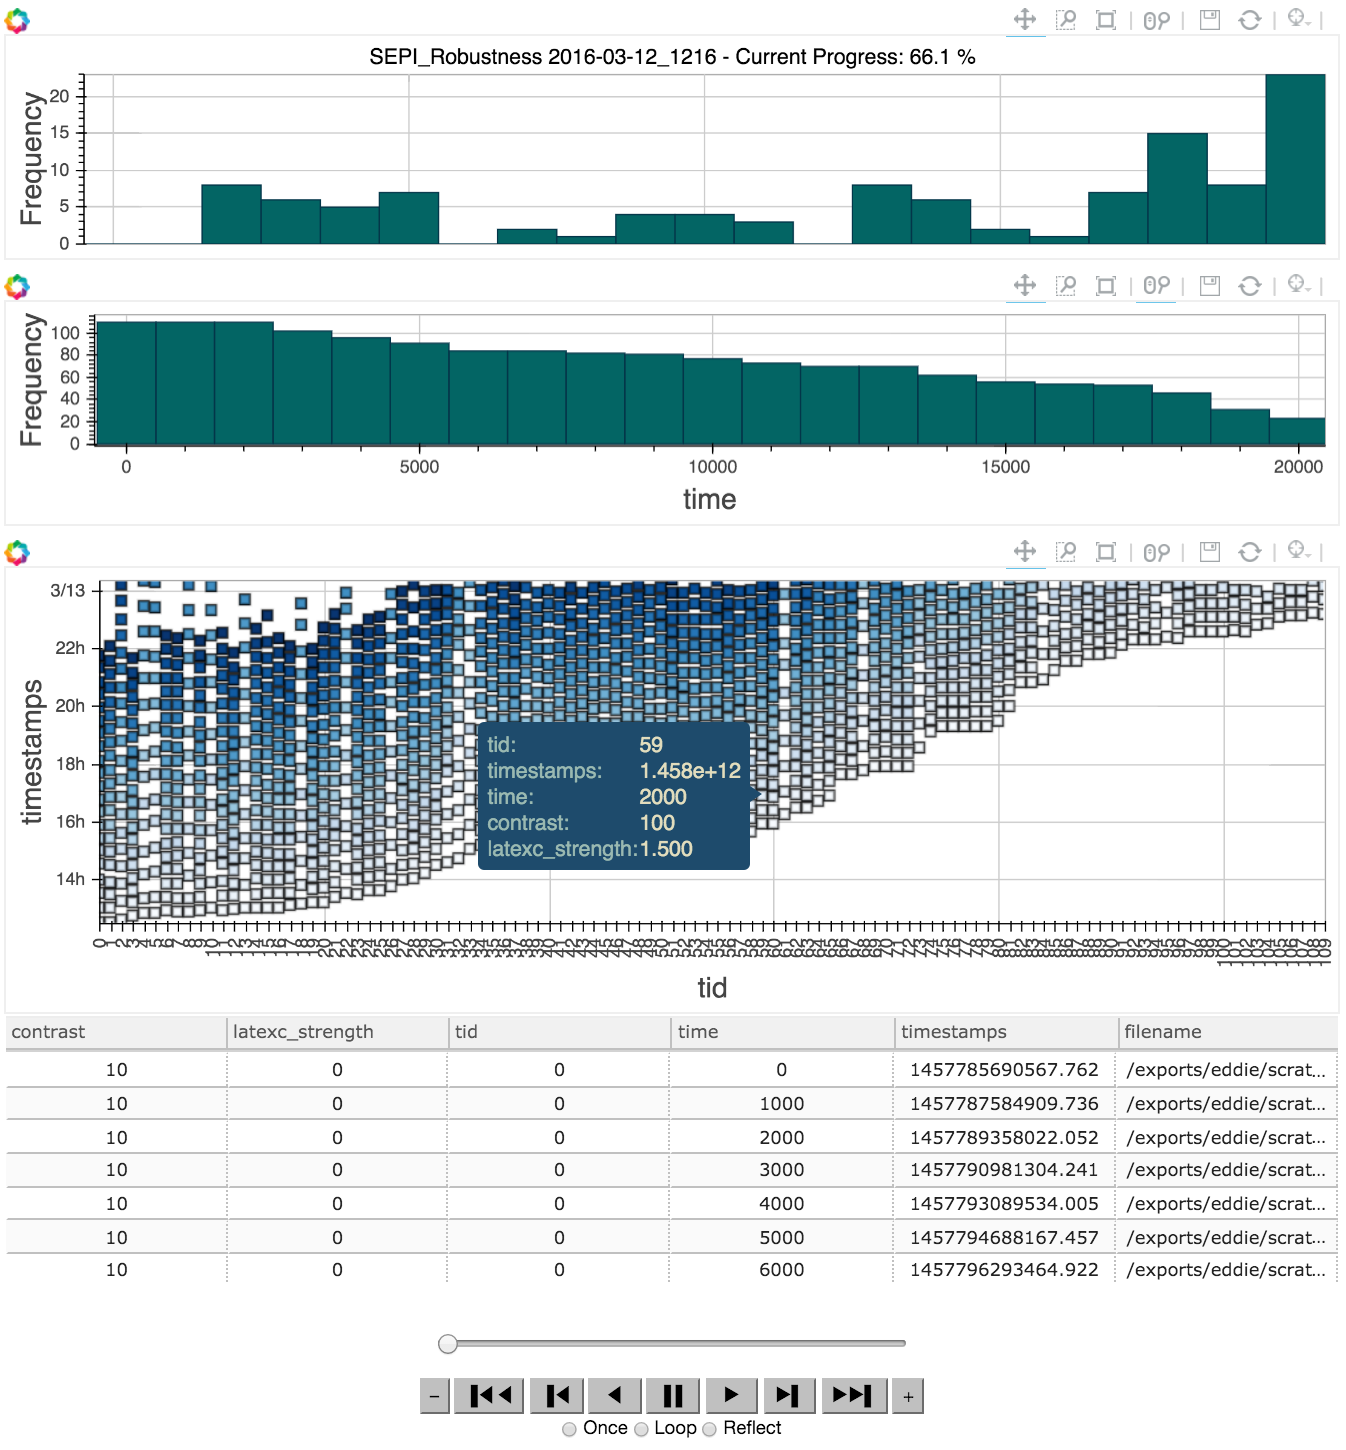
\includegraphics[width=1.0\textwidth]{workflow_progress.png}
	    \caption[Interactive dashboard to monitor workflow
          progress.]{Interactive real time dashboard to monitor the
          progress of an experiment and catch any problems or failures
          in individual jobs. Top panel shows current progress in
          developmental time, second panel shows completion at each
          time. Third panel plots the times at which each part of a
          job completed.}
	\label{workflow_progress}
\end{figure}


\subsection{Step 5: Loading results}

A core part of the workflow is linking up the output generated by
Lancet with the data structures provided by HoloViews. In order to
make this easy the user can specify a file pattern to search for
generated files, which can be loaded into a Table. The Table can then
be expanded into another HoloViews datastructure called a Layout,
which makes it possible to access individual measurements or analyses
without having to load the whole file. This means that with just a
single line of code we can specify precisely which measurement and
which part of the parameter space to load and visualize it immediately
using interactive widgets and complex plot arrangements.

Each measurement or analysis can be accessed via a tree-like
structure, letting us access individual measurements by accessing them
with attribute access and selecting by the parameter values.

\begin{minipage}{\linewidth}
\begin{lstlisting}
  :Layout
   .CFs.LateralInhibitory     :Collator   [Index,contrast,latexc_strength,tid,time,timestamps]   (filename,entries)
   .CFs.LateralExcitatory     :Collator   [Index,contrast,latexc_strength,tid,time,timestamps]   (filename,entries)
   .OrientationPreference.V1  :Collator   [Index,contrast,latexc_strength,tid,time,timestamps]   (filename,entries)
   .OrientationSelectivity.V1 :Collator   [Index,contrast,latexc_strength,tid,time,timestamps]   (filename,entries)
\end{lstlisting}
\end{minipage}


\begin{figure}
	\centering
        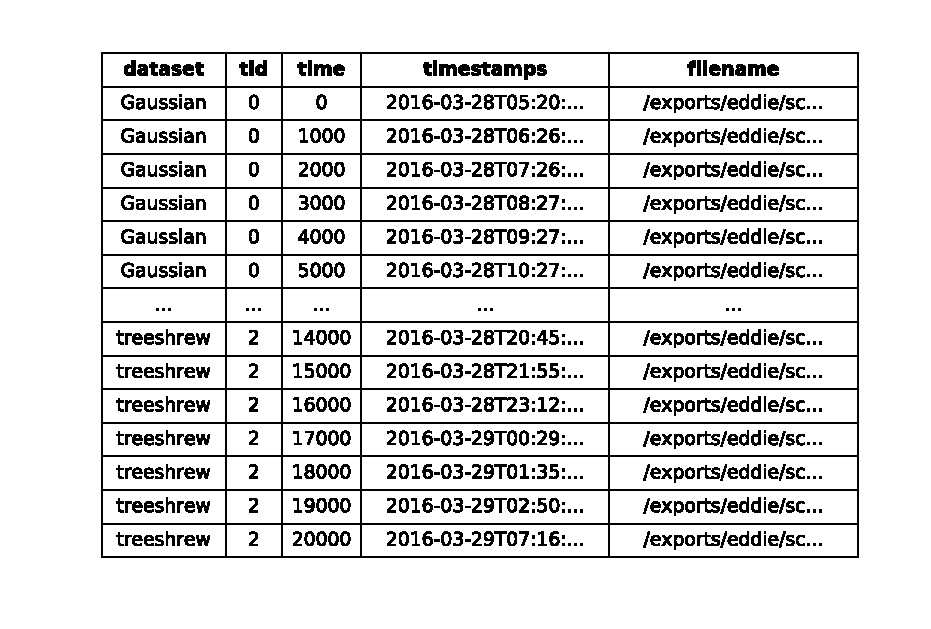
\includegraphics[width=0.7\textwidth]{workflow_load.pdf}
	    \caption[Table summarizing results from parameter analysis in
          Lancet and HoloViews.]{Table showing the output of a
          parameter exploration using Lancet and HoloViews. Each row
          represents one file of measurement results. The Table allows
          selecting just the subset of files to be loaded.}
	\label{workflow_load}
\end{figure}


\subsection{Step 6: Analysis and Visualization}

The exploratory analysis and visualization of a dataset is one of the
most important aspect of a scientists workflow. However, traditional
analysis and visualization libraries split those two aspects such,
which provides a significant bottleneck to what the user actually
wants to do, namely to understand their data. By giving data elements
their own visual representation we can provide immediate visual
feedback, while still making all the data available for further
processing. Additionally HoloViews provides containers and other
datastructures that automatically get translated into complex plot
arrangements and widgets making it trivial to explore datasets of any
dimensionality and complexity.

In the previous step we saw how to load a dataset, here we will
quickly demonstrate how we can work with this data once it is loaded.
As an example we load some of the weights that represent synaptic
neural connections between different neurons in our model. In
Figure~\ref{workflow_explore} we can see how we can load two sets of
weights for a specific set of parameters and compose them together by
overlaying them. The resulting visualization demonstrates the
complexity this approach allows as we can represent the X/Y positions
of the neurons in the V1 sheet on a grid, while representing other
dimensions such as the lateral excitatory strength and contrast as
sliders. Such a plot would usually be very complex to construct but
here it is just a side-effect of the way the data has been structured
and annotated and we could easily transform the dataset to slice and
visualize it in any number of ways. Furthermore all the underlying
weights are easily accessible and we can therefore feed this data
structure straight into further analysis function.

Combining visualization and analysis in this proves to be an
incredibly powerful paradigm to work with large datasets. The main
benefits are that the user no longer has to manually keep track of
metadata, which means that plots automatically generate appropriate
labels and the analysis code always has access to all the information
it requires. This also means that instead of storing a plot in an
unreproducible format, the full specification of the plot including
data, metadata and styling details can be stored as a single object,
which can be loaded later to extract the raw data or merely to
reproduce the plot.

\begin{figure}
	\centering
        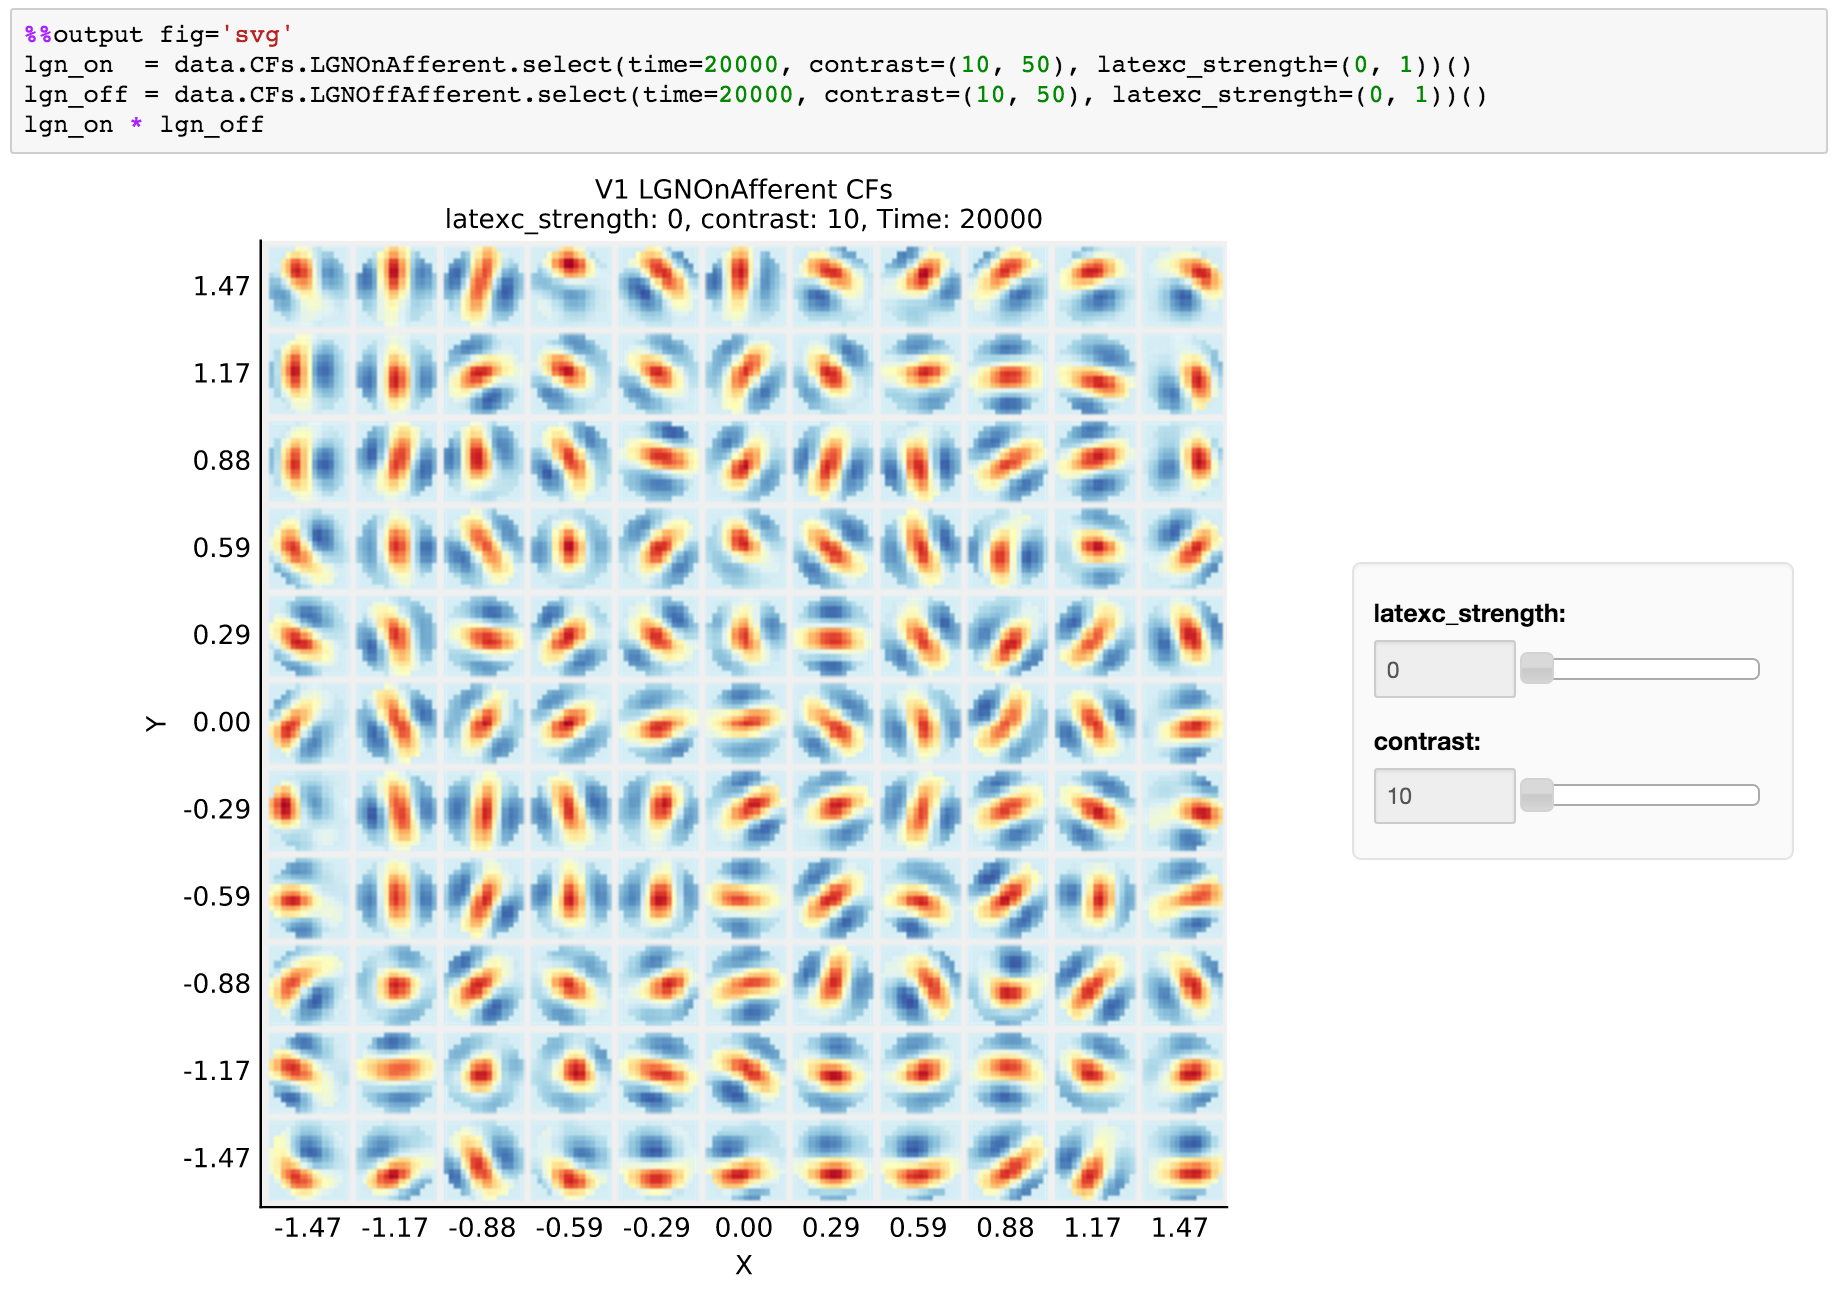
\includegraphics[width=1.0\textwidth]{workflow_explore.png}
	\caption[Demonstration of complex parameter exploration in
      HoloViews.]{Demonstration of loading a measurement from the
      parameter exploration showing the afferent weights of the model
      varying across the parameter space we defined for the
      experiment. Through the use of multi-dimensional datastructures
      we can achieve complex plotting arrangements and explore any
      further data dimensions using widgets, which appear
      automatically.}
	\label{workflow_explore}
\end{figure}

\subsection{Step 7: Visual aesthetics and publication quality plotting}

The flexibility of HoloViews not only allows for quick data
exploration but even extends to generating publication quality
figures. As stated previously all plots used as part of this thesis
were generated using HoloViews and each chapter is accompanied by
notebooks, which replicate the entire workflow. This is made possible
because HoloViews allows for huge flexibility in customizing the
automatically generated visual representations.

\section{Summary}

In this chapter we have demonstrated a complete workflow for the
specification, launching, collection, exploration and visualization of
a computational experiment developed for this thesis. It provides huge
benefits in terms of usability and reproducibility over previous
approaches since it captures the full breadth of an individual
research project keeping a complete record of everything required to
reproduce both the data and the actual published figures and is now
used in research projects in research projects ranging from
neuroscience \citep{Keemink2015} to physics \citep{Nijholt2015,
  Tenner2016}, astronomy, meteorology, and chemistry.

 %
%!TEX root = ../PhDthesis.tex
\chapter{A spatially calibrated model of visual cortex}
\label{SCALmodel}

One of the major obstacles in modern neuroscience is integrating the
vast amount of experimental data that has been generated, highlighting
where different sources of evidence is and is not in agreement and
offering testable hypothesis to resolve such discrepancies. The
primary visual cortex is one of the most well studied areas in the
mammalian brain and we have previously seen that it has been
extensively explored at varying levels of description, from
development, circuits and anatomy to surround modulation, behavioral
studies and theoretical models of computation.

In order to provide a better account on how all this information fits
together in a generalized model describing the organization and
computations performed by the cortex, a unified reference frame
regarding the various spatial scales is desperately needed. A careful
reading of the literature highlights just how dependent various
effects are on the spatial profiles of the underlying neurite
projections. Here I will present a developmental model that takes
these levels of evidence into account, allowing us to cross-validate
known anatomical properties by confirming them against the response
properties of the model after development. This will allow bridging
between known measurements of anatomy and circuitry and
electro-physiological or even behavioral experiments performed on
visual cortex.

So far only very few attempts have been made at developing models that
take into account the various spatial properties that have been
described in the literature ranging from anatomy to
electro-physiological measurements. This chapter will demonstrate how
existing models of cortical development, specifically the Gain Control
Adaptation Lateral model (GCAL) \citep{Stevens2013} can be calibrated
to match known measurements of spatial extents more closely in a new
\textbf{S}patially \textbf{CAL}ibrated (SCAL) model.

The analysis will focus on various experimental assessments of the
spatial properties of the visual pathway and describe how we can use
these to build a model that achieves a high-level of consistency with
experimental results across a wide range of measures. Specifically,
the model will be calibrated with experimental measurements in the
parafoveal regions of the visual system of macaque. The macaque has
long been a experimental model for in visual neuroscience and the
literature surrounding contextual modulation in particular. In doing
so this chapter will critically evaluate the literature surrounding
spatial tuning properties in the mammalian cortex, highlighting
discrepancies and specifically assessing various models used to
characterize the spatial tuning properties of neurons in the visual
pathway.

Once we have collected the data we will provide a full
characterization of the spatial response properties, receptive fields
and synaptic weights in the model confirming they closely match
experimental data. At the same time we will outline in which ways the
model falls short and discuss some ways in which these shortcomings
might be remedied, which we will pick up in the following chapters.
In particular we will highlight problems with the classical GCAL
architecture, which makes no distinction between excitatory and
inhibitory cell classes and how that relates to the spatial
calibration and long-range surround suppression, which is thought to
be mediated by disynaptic, long-range excitatory mechanisms.

\section{Methods}

In this chapter we first introduce the developmental models of the
primary visual cortex the more complex models are based on. We begin
by outlining the equations and mechanisms underpinning these models
and then describe various analyses we can apply to these models to
replicate experimental protocols and compare the model against
experimental results.

\subsection{A spatially calibrated model of cortical development} 

The GCAL model put forth in \cite{Stevens2013} will serve as the
starting point for the models in this thesis. As discussed previously
(see Section \ref{devmodels}), it provides the first model that
develops robust and stable orientation maps independent of visual
contrast and for a wide range of training inputs. In this section we
describe the equations governing this model, how it is structured and
will highlight the modifications that were made to achieve a more
consistent spatial calibration.

The major changes introduced in this model are the replacement of
subtractive with divisive inhibition and large changes to the spatial
profile of connections. One of the major issues we will attempt to
settle here is whether the formation of orientation maps requires real
long-range inhibitory connections or whether the extents of known
inhibitory cell classes is sufficient to account the development of
smooth and robust orientation maps. Additionally we add an optional
long-range excitatory connection to the model to determine if the
model develops in a realistic manner. Before analyzing the behavior of
the model we describe its overall architecture and the equations
governing its behavior.

\subsubsection*{Architecture}

The architecture of this family of models builds on two main concepts,
the idea of 2D sheets of firing-rate point neurons and projections
between them, representing the synaptic connections between the
neurons. All models we will introduce share the same basic
organization at the retinal and lateral geniculate nucleus level, but
we will introduce increasingly complex models of the interactions in
the primary visual cortex. In Figure~\ref{LGNDiagram} you can see the
organization of the retinal and lateral geniculate nucleus ON and OFF
sheets.

\begin{figure}
	\centering
        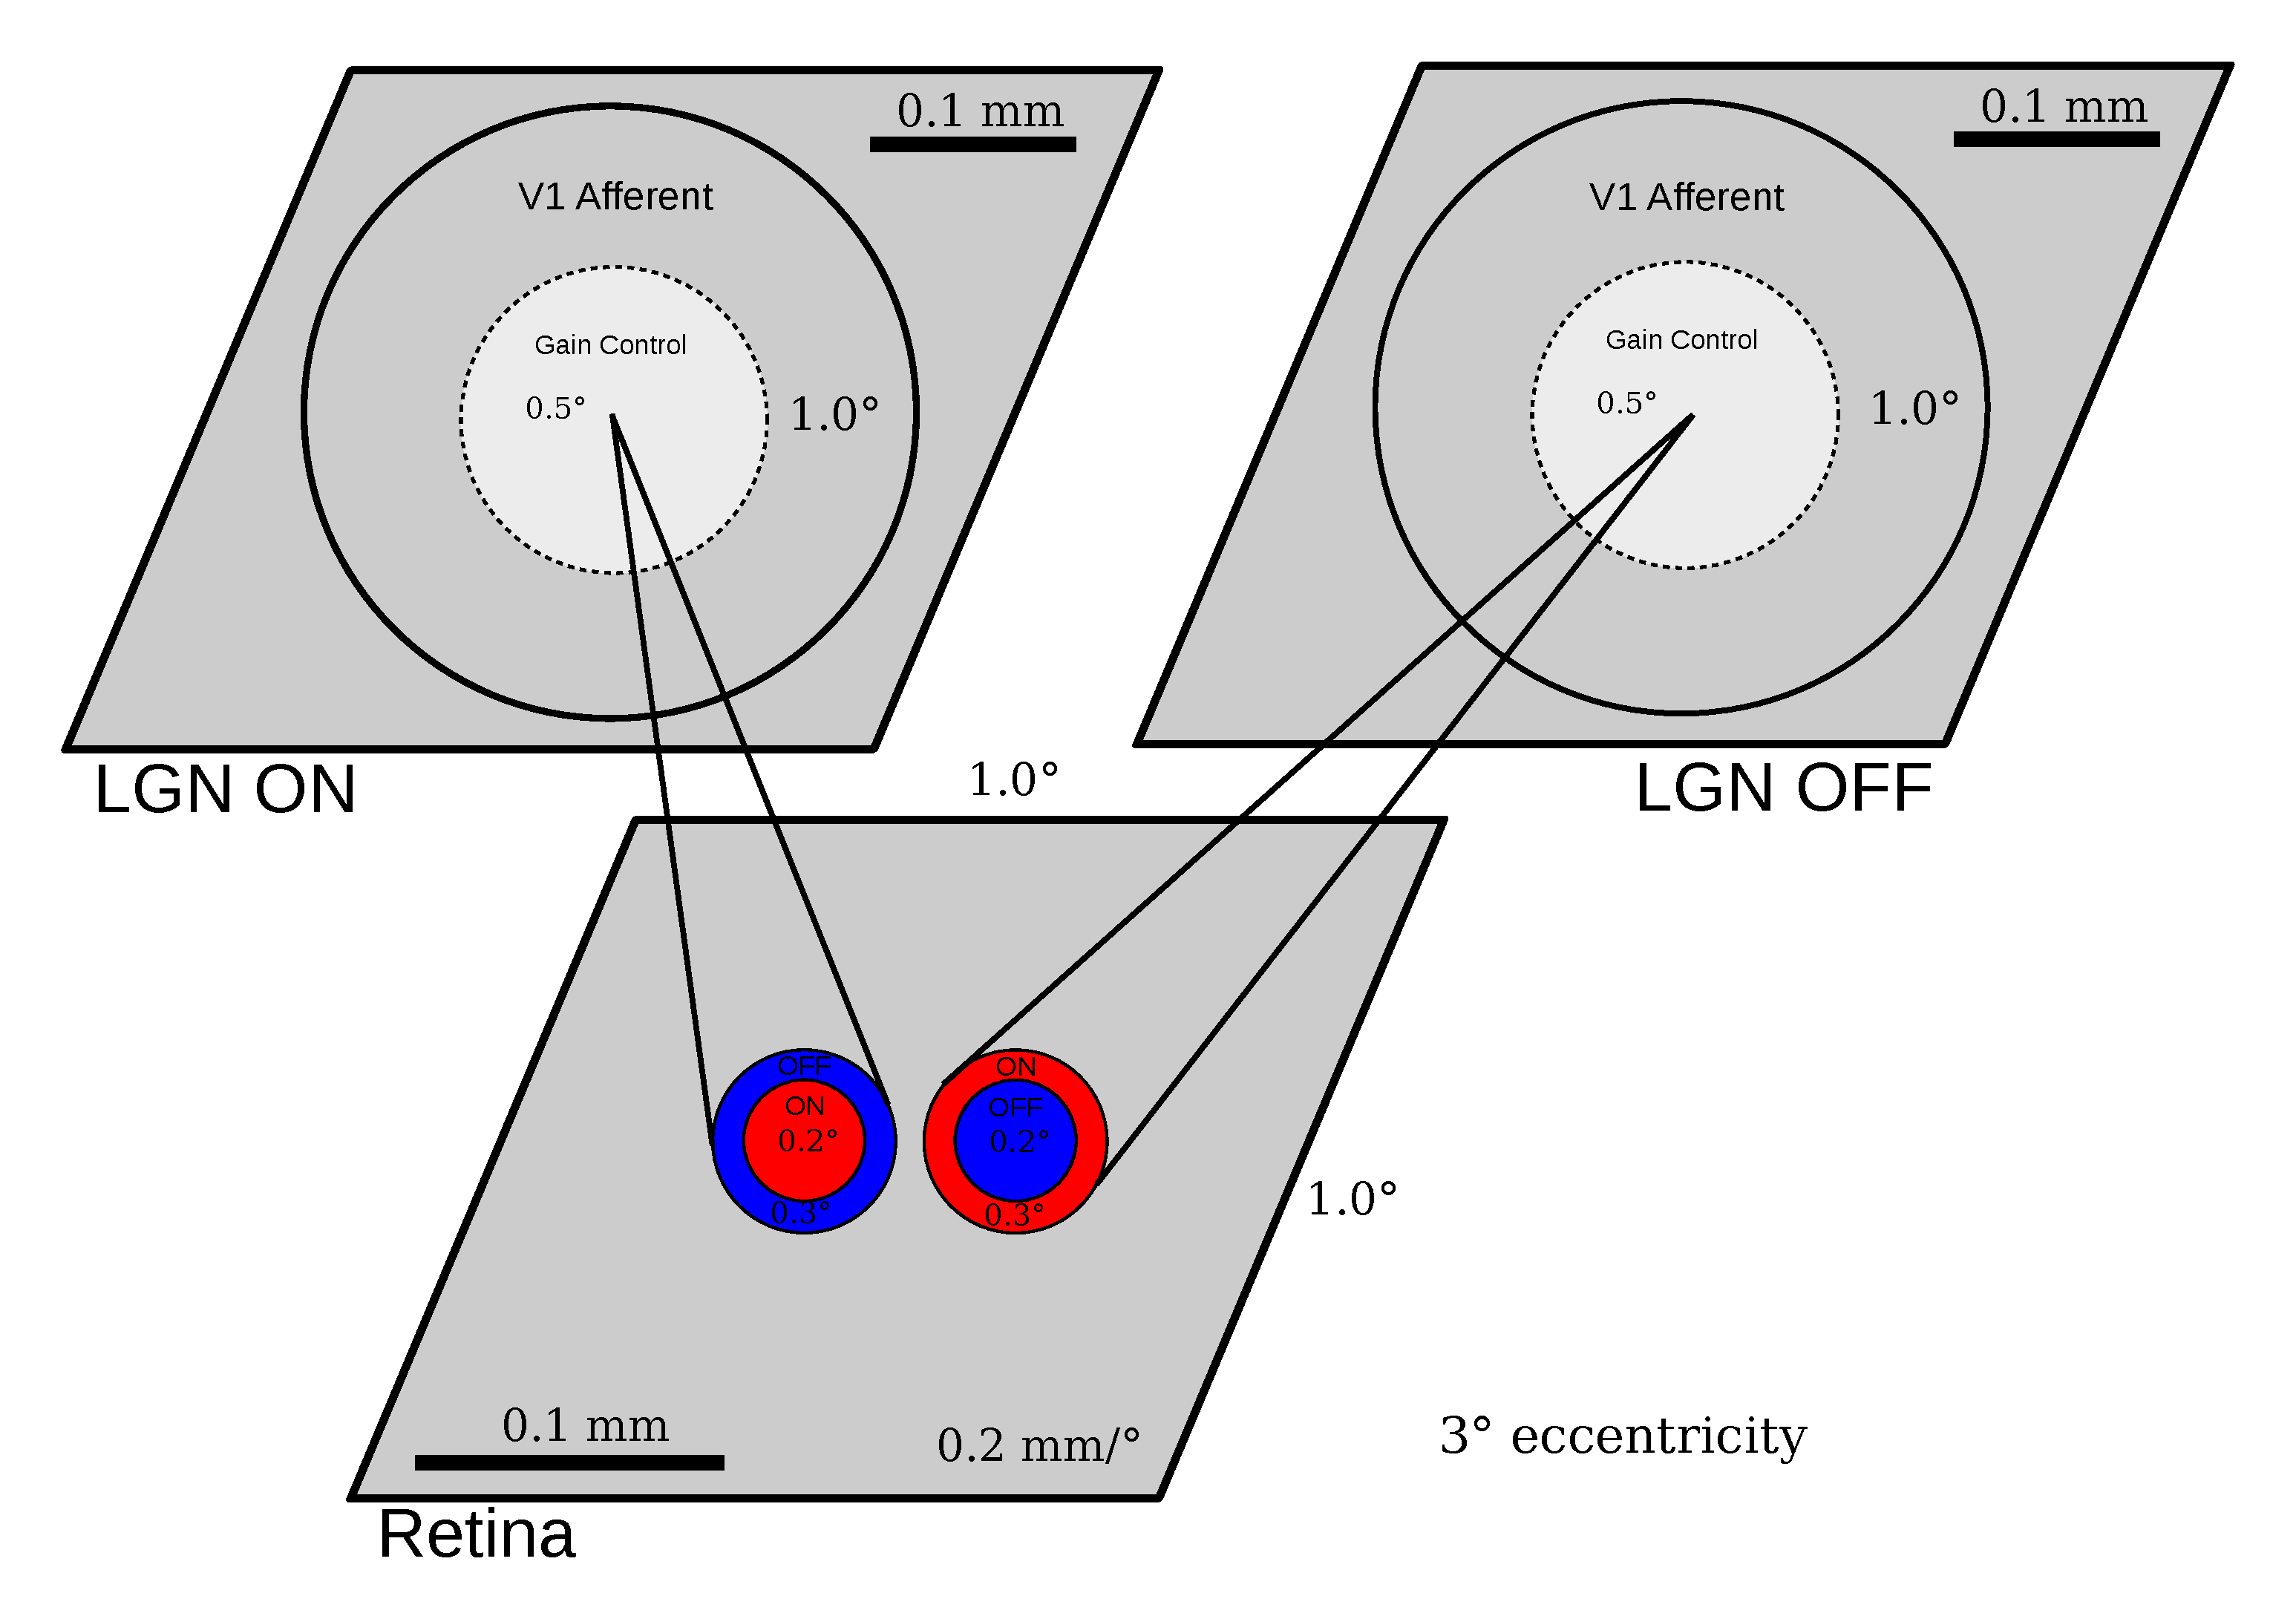
\includegraphics[width=1.0\textwidth]{LGN_Diagram.pdf}
	\caption[Diagram of the SCAL retinogeniculate stage.]{Diagram of
      the retinogeniculate stages of the spatially calibrated (SCAL)
      model. At the LGN level the excitatory and inhibitory
      center-surround components are shown in red and blue
      respectively. In the LGN the absolute size of the divisive gain
      control connection is indicated by a solid line while the
      diameter of the Gaussian used to initialize the lateral weights
      is marked by a dotted line. The given spatial scales hold for an
      eccentricity of 3\degree in macaque retina and LGN.}
	\label{LGNDiagram}
\end{figure}

The model operates by presenting patterns on the retinal sheet, which
then get filtered through difference-of-gaussian connection fields,
which give rise to the response the ON and OFF sheets. There a lateral
gain control projection applies some pooling normalization to the
response. This early stage of processing represents a crude model of
retinal ganglion and LGN function and provides the input to the
various cortical models introduced here.

The architecture of the retinal ganglion cell and lateral geniculate
nucleus layers will remain unchanged for all the models presented in
this thesis, while the V1 stage will be progressively refined.

The model diagram for the SCAL V1 stage is shown in
Figure~\ref{SCALDiagram} consisting of a single neural sheet with a
comparatively large afferent connection when considered against the
GCAL model. The local excitatory and inhibitory kernels however have
changed only slightly in their size and finally the model optionally
includes a long-range excitatory connection, which represents the
long-range patchy lateral connectivity that is so characteristic of
layer 2/3 in the visual cortex of higher mammals.

\begin{figure}
	\centering
        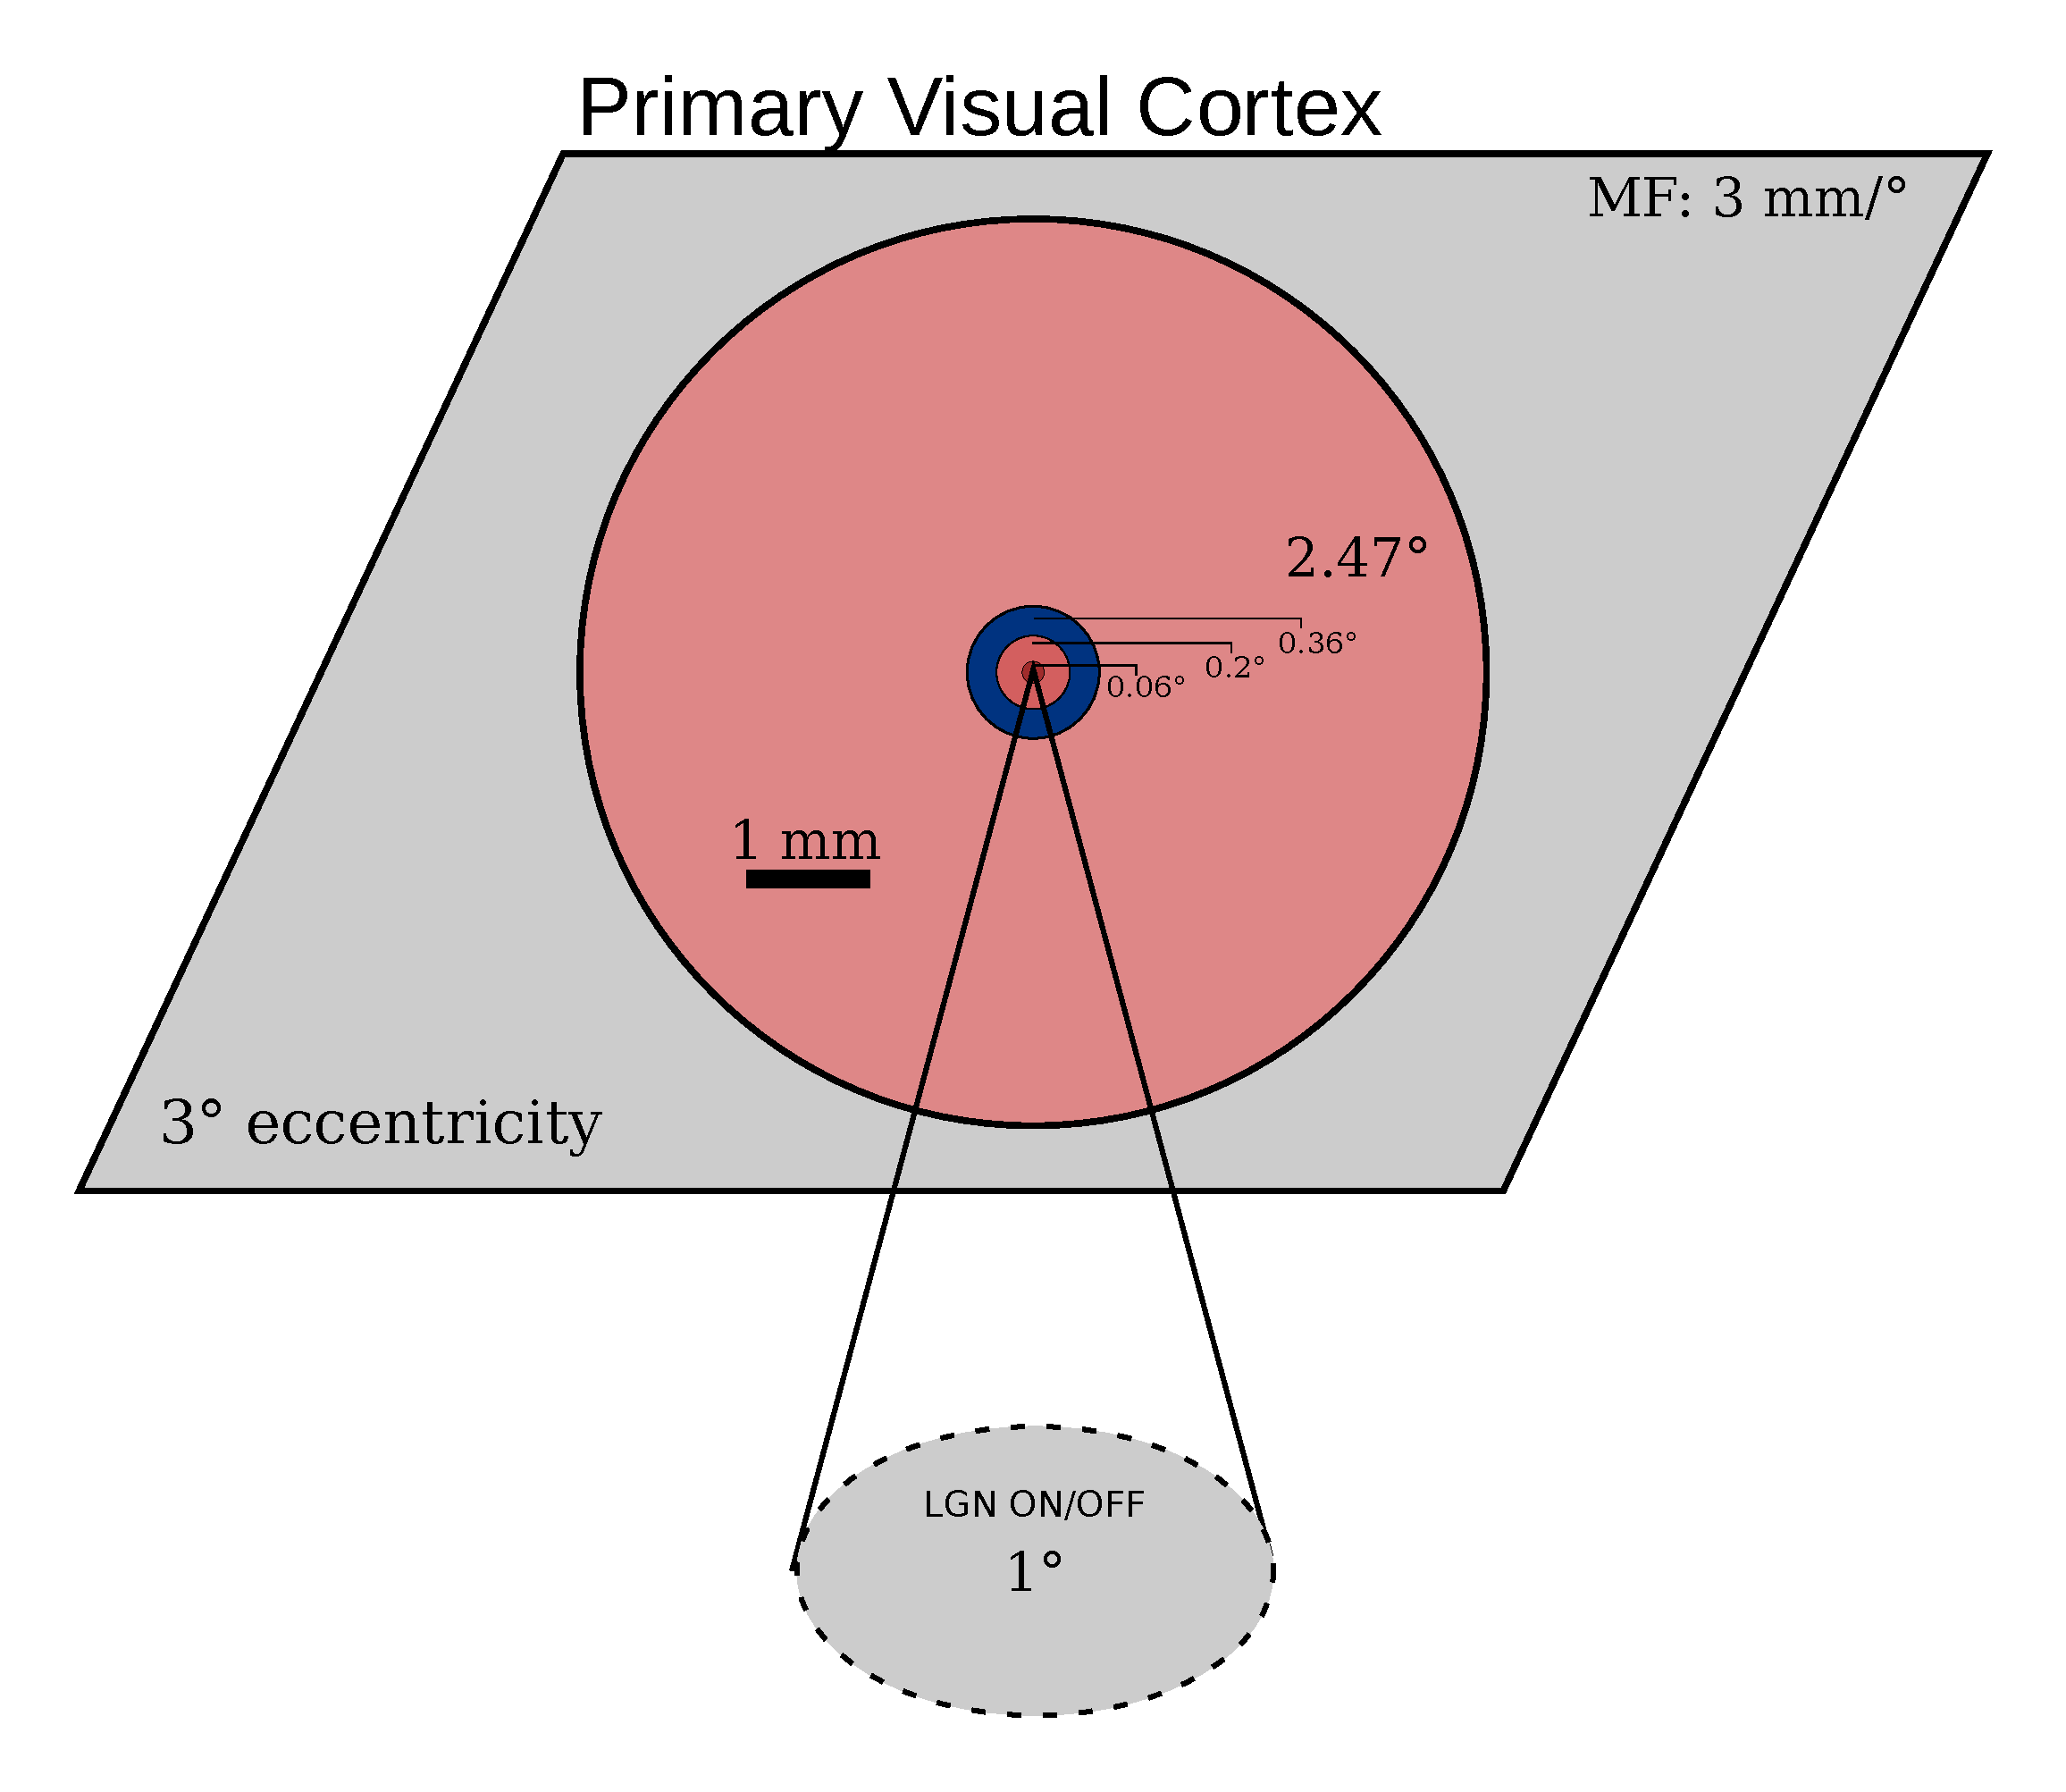
\includegraphics[width=1.0\textwidth]{SCAL_Diagram.pdf}
	\caption[Schematic representation of the SCAL model.]{Diagram of
      the SCAL V1 stage of the model showing the spatial scales of the
      various excitatory (red) and inhibitory (blue)
      connections. Saturated colors indicate the kernel radii, while
      lightly shaded regions indicate kernel cut-off extents.}
	\label{SCALDiagram}
\end{figure}

\subsubsection*{Input patterns}

The organization of the self-organizing map (SOM) based developmental
models of the cortex, is determined by a complex interplay between the
model and the input patterns it is trained on. Just as in the
developing brain connections are formed depending on the statistics of
the sensory experience of the strongly influencing the spatial
organization of the model. In order to accurately assess how the
models respond to and self-organize in different visual environments
we will use three different visual stimuli to present to the model,
however the results in this chapter will be based purely on the simple
Gaussian stimuli.

These patterns, used as the baseline for most measurements, are simply
elongated Gaussian shapes matching the length of the integrative area
of a V1 neuron and with a spatial frequency that would allow three
distinct lobes to form within this area. The training patterns are
given by:
%%
\begin{equation}
  exp(-x^2/(2\sigma_x^2) - y^2/(2\sigma_y^2)
\label{eqn:gausspattern}
\end{equation}
%%
Additionally two image datasets will be employed one taken from a
database of natural images and the other recorded from within the
rearing environment of ferrets in a laboratory, which is dominated by
the long co-linear statistics of the cage bars. These datasets will
allow us to explore the effect of the natural image statistics on the
organization of the models and confirm robustness against a wide range
of visual input.

\subsubsection*{Activation}

All the models operate by presenting a new retinal input at each
iteration updating the activation of each unit in each sheet. The
neurons in the sheets are firing-rate point neurons, with the main
state being a floating point activation value.  For all models, the
activation level $\eta$ for a unit at position $j$ in an ON/OFF sheet
O at time $t+\delta t$ is defined as:
%%
\begin{equation}
\eta_{j, O}(t+\delta t)=f\left(\frac{\gamma_{O}\sum_{i\in
    F_{j,P}}\Psi_{i}(t)\omega_{ij}}{k+\gamma_{S}\sum_{i\in
    F_{j,S}}\eta_{i, O}(t)\omega_{ij, S}}\right)
\label{eqn:lgnactivation}
\end{equation}
%%
The constant $\gamma_{O}=14.0$ is an arbitrary multiplier for the
overall strength of connections from the photoreceptor sheet to the
ON/OFF sheets, chosen to give typical activations in the range 0.0 to
1.0, while $\gamma_{S}$ is the strength of the feed-forward
contrast-gain control. $\Psi_{i}$ is the activation of unit $i$ in the
two-dimensional array of neurons on the photoreceptor sheet from which
ON/OFF unit $j$ receives input (its afferent connection field
$F_{j,P}$) and $\eta_{i, O}(t)$ is the activation of other ON/OFF
units on the previous time step (received over the suppressive
connection field $F_{j,S}$). The activation function $f$ is a
half-wave rectifying function that ensures the activation of ON/OFF
units is always positive.

The weights $\omega_{ij}$ represent the fixed connection weights from
photoreceptor $i$ to the ON or OFF unit $j$ defined with a standard
difference-of-Gaussians (DoG) kernel. The connection fields for ON units
have a positive center and negative surround, and vice versa for OFF
units. More precisely, the weight $\omega_{ij}$ from an ON-center cell
at location (0,0) in the ON sheet and a photoreceptor sheet in
location $(x,y)$ on the photoreceptor sheet is given by:
%%
\begin{equation}
\omega_{ij}=\frac{1}{Z_c}\exp{\left(-\frac{x^{2}+y^{2}}{2\sigma_{c}^{2}}\right)}-\frac{1}{Z_s}\exp\left(-\frac{x^{2}+y^{2}}{2\sigma_{s}^{2}}\right)
\label{eqn:DoG}
\end{equation}
%%
The kernel sizes of the central Gaussian $\sigma_{c}$ and surround
mechanism $\sigma_{s}$ are what we will be determining here. Unlike
simple DoG kernels, the center-surround are jointly normalized to 1.0
using $Z_c$ and $Z_s$. The weights for an OFF-center cell are the
negative of the ON-center weights (i.e., surround minus center). The
center of the connection field of each ON/OFF unit is mapped to the
location in the photoreceptor sheet corresponding to the location of
that unit in sheet coordinates, making the projection retinotopic.

The weights $\omega_{ij, S}$ in the denominator of
equation~\ref{eqn:lgnactivation} specify the spatial profile of the
lateral inhibition received from other ON/OFF units when contrast-gain
control is active. The weights of these connections have a fixed,
circular Gaussian profile so that for a neuron located at (0,0) in
either the ON or OFF sheet:
%%
\begin{equation}
\omega_{ij,S}=\frac{1}{Z_S}\exp\left(-\frac{x^{2}+y^{2}}{2\sigma_{S}^{2}}\right)
\label{eqn:gauss}
\end{equation}
%%
where $(x, y)$ is the location of the pre-synaptic neuron, $\sigma_{S}$
determines the width of the Gaussian, and $Z_S$ is a normalizing
constant that ensures that the total of all the lateral inhibitory
weights $\omega_{ij}$ to neuron $j$ sum to 1.0. This gain-control
projection is activated once per iteration before activity is sent to
the V1 sheet.

\subsubsection*{The V1 model}

As we saw above in the LGN section the model described here is heavily
based on the GCAL model \citep{Stevens2013}, however it does differ in
one major respect---it employs divisive rather than subtractive
inhibition. Here we will describe the equations that govern the model
and point out where they differ to previous models.

Each V1 neuron in each model receives connections from three different
connection types or `projections' ($p$), i.e., the afferent projection
from the ON/OFF sheets (both channels concatenated into one input
vector; $p=A$), the recurrent lateral excitatory projection ($p=E$),
and the recurrent lateral inhibitory projection ($p=I$) from other V1
neurons.

The contribution $C_{j,p}$ to the activation of unit $j$ from each
projection type ($p=A,E,I$) is calculated as:
%%
\begin{equation}
C_{j,p}(t+\delta t)=\sum_{i\in F_{j,p}}\eta_{i, p}(t)\omega_{ij,p}
\label{eqn:update}
\end{equation}
%%
where $\eta_{i, p}$ is the activation of unit $i$ taken from the set
of neurons in V1 to which unit $j$ is connected (its connection field
$F_j$) and $w_{ij,p}$ is the connection weight from unit $i$ in V1 to
unit $j$ in V1 for the projection $p$. Afferent activity ($p=A$)
remains constant after the first update from the retina, but the other
contributions change over 16 settling steps, depending on the activity
in V1.

The contributions from all three projections to V1 (afferent
($p_{A}$), excitatory $p_{E}$ and inhibitory $p_{I}$) described above
are combined using equation~\ref{eqn:activation1} to calculate the
activation of a neuron $j$ in V1 at time t:
%%
\begin{equation}
\eta_{j,V}(t)=f\left(\frac{\sum_{p=\{E, A\}}\gamma_{p}C_{jp}(t)}{1+\sum_{p=\{I\}}\gamma_{p}C_{jp}(t)}\right)
\label{eqn:activation1}
\end{equation}
%%
The projection strength scaling factors $\gamma$ are defined for each
projection type set to provide a balance between excitation and
inhibition, and between afferent and lateral influences, to provide
robust formation of activity bubbles that allows smooth maps to
form. The function $f$ defines a variable threshold point ($\theta$)
dependent on the average activity of the unit as described in the next
subsection, but in all cases the gain is fixed at unity. Note that
unlike GCAL the inhibitory projection acts divisively rather than
subtractively.

At the end of the 16 settling steps, the settled V1 activation pattern
is deemed to be the V1 response to the presented pattern. At this
point we use the V1 response to update the threshold point ($\theta$)
of V1 neurons (using the adaptation process described below) and to
update the afferent and lateral inhibitory weights via Hebbian
learning. Unlike the regular GCAL model the V1 activity is not reset
to zero instead being allowed to decay until the onset of the next
visual input pattern.

In order to assess the development of long-range patchy connections in
this model we additionally add a long-range excitatory connection,
which we let develop without any weight. This term is modeled as an
additional multiplicative component with a constant offset of 1,
ensuring only facilitatory modulation from the far surround. The
activation of a model neuron is therefore given by:
%%
\begin{equation}
  \eta_{exc} = \frac{\eta_{A} + \eta_{E}}{1 + \eta_{I}}
\end{equation}
%%
where $\eta_A$ is the afferent activity, $\eta_E$ is the local
excitatory input, $\eta_I$ is the divisive inhibitory input and
$\eta_{LR}$ is the long-range excitatory input.

\subsection*{Adaptation}

In order to set the threshold for activation, each neuron unit $j$ in
V1 calculates a smoothed exponential average of its settled activity
patterns ($\overline{\eta_{j}}$):
%%
\begin{equation}
\overline{\eta_{j}}(t)= (1-\beta)\eta_{j}(t) + \beta\overline{\eta_{j}}(t-1)
\label{eqn:averaging}
\end{equation}
%%
The smoothing parameter ($\beta=0.991$) determines the degree of
smoothing in the calculation of the average. $\overline{\eta_{j}}$ is
initialized to the target average V1 unit activity ($\mu$), which for
all simulations is $\overline{\eta_{jA}}(0) = \mu= 0.024$. The
threshold is updated using:
%%
\begin{equation}
\label{eqn:thresholdupdate}%
\theta(t)= \theta(t-1) + \lambda(\overline{\eta_{j}}(t) -\mu)
\end{equation}
%%
where $\lambda=0.01$ is the homeostatic learning rate. The effect of
this scaling mechanism is to bring the average activity of each V1
unit closer to the specified target. If the activity in a V1 unit
moves away from the target during training, the threshold for
activation is thus automatically raised or lowered in order to bring
it closer to the target. Note that an alternative rule with only a
single smoothing parameter (rather than $\beta$ and $\lambda$) could
be formulated, but the rule as presented here makes it simple for the
modeler to set a desired target activity $\mu$.

\subsection*{Learning}

Initial connection field weights are isotropic 2D Gaussians for the
lateral excitatory projection and uniformly random within a Gaussian
envelope for afferent and lateral inhibitory
projections. Specifically, for a neuron located at (0,0):
%%
\begin{equation}
\omega_{ij}=\frac{1}{Z_p}u\exp\left(-\frac{x^{2}+y^{2}}{2\sigma_{p}^{2}}\right)
\label{eqn:gaussrandomweights}
\end{equation}
%%
where $(x, y)$ is the sheet-coordinate location of the pre-synaptic
neuron, $u=1$ for the lateral excitatory projection ($p=E$) and $u$ is
a scalar value drawn from a uniform random distribution for the
afferent and lateral inhibitory projections ($p=A,I$), $\sigma_{p}$
determines the width of the Gaussian in sheet coordinates, which
correspond to visual degrees in the spatially calibrated model. For a
full summary for the parameters of the model see Appendix
\ref{Appendix:Parameters}.

In the model, as images are presented to
the photoreceptors, V1 afferent connection weights $\omega_{ij,A}$
from the ON/OFF sheets are adjusted once per iteration (after V1
settling is completed) using a simple Hebbian learning rule. This rule
results in connections that reflect correlations between the
pre-synaptic ON/OFF unit activities and the post-synaptic V1 response.
Hebbian connection weight adjustment at each iteration is dependent on
the pre-synaptic activity, the post-synaptic response, and the Hebbian
learning rate:
%%
\begin{equation}
\omega_{ij,p}(t)=\frac{\omega_{ij,p}(t-1)+\alpha\eta_{j}\eta_{i}}{\sum_{k}\left(\omega_{kj,p}(t-1)+\alpha\eta_{j}\eta_{k}\right)}
\label{eqn:hebb}
\end{equation}
%%
where for unit $j$, $\alpha$ is the Hebbian learning rate for the
afferent connection field $F_{j}$. Unless it is constrained, Hebbian
learning will lead to ever-increasing (and thus unstable) values of
the weights \citep{Rochester1956}. In all the models the weights are
constrained using divisive post-synaptic weight normalization
(equation~\ref{eqn:hebb}), which is a simple and well understood
mechanism. Afferent connection weights from ON and OFF units are
normalized together in the model. We expect that a more biologically
motivated homeostatic mechanism for normalization such as
multiplicative synaptic scaling
\citep{Turrigiano1999,Turrigiano2004,Sullivan2006} or a sliding
threshold for plasticity \citep{Bienenstock1982} would achieve similar
results, but have not tested these.

The learning rates $\alpha$ are defined separately for the afferent,
lateral excitatory and lateral inhibitory projections. The
density-specific value used in the equation above is then calculated
as $\alpha=\frac{\alpha_{A}}{\tau_{A}}$, where $\tau_{A}$ is the
number of connections per connection field in the afferent projection.


\subsection{Measurements}

Measurements in the model are performed by presenting patterns varying
by one or more features and computing the maximum response across one
or more of those features. This closely matches the protocol usually
employed in experiments ranging from optical imaging to measure
orientation maps and electrophysiological measurements to capture
individual tuning curves.

\subsubsection*{Orientation tuning} \label{ORMeasurement}

The orientation map measurements in the model follow the procedure by
\cite{Blasdel1992}, presenting sine gratings at 12 different
orientations and 18 different phases computing computing the vector
average across the phases and returning the phase averaged orientation
preference and selectivity maps. Since the model does not have
direction tuning or complex cells each phase is presented individually
rather than as directionally drifting gratings as is usually done in
experiments.

\subsubsection*{Size tuning}

The size-tuning measurements are modeled on the measurements by
\cite{Sceniak1999} and \cite{Sceniak2001} presenting sine grating
stimuli of increasing area at the preferred position, orientation and
spatial frequency of the central neuron. Due to the uncertainty in
experimental measurements we can include all neurons within
0.1\degree\ of central neurons, which respond significantly and have
an orientation preference varying from the central neuron by no more
than $\pi/16$ radians.

The low and high contrast values were chosen to fall into the lower
linear region and just below the saturation point of the contrast
response curve respectively.

\subsubsection*{Frequency tuning}

The frequency tuning measurements were performed the same way as the
size-tuning measurements, but instead of optimizing the spatial
frequency of the pattern it was varied. The size of the stimulus was
restricted to a 2x2\degree\ region in the retina centered around the
measured neurons.

\subsection{Analyses}

In order to analyze the spatial organization of the developed model we
borrow from a variety of techniques used to analyze
electrophysiological, optical imaging and anatomical data obtained in
vivo allowing us to compare directly between experimental results and
our model.

\subsubsection*x{Area summation curves} \label{DoG_Section}

The area summation curves were measured in the model by presenting the
model with disks of sine gratings of increasing size and varying phase
and at the optimal spatial frequency of each neuron. The size-tuning
curves obtained in this way were then fitted with the integrated
Difference-of-Gaussian model described by the following equation:
%%
\begin{equation}
R(s) = R_0 + K_e \int \int re^{-\frac{r^2}{a}} \,
\mathrm{d}r\mathrm{d}\theta - K_i \int\int re^{-\frac{r^2}{b}} \,
\mathrm{d}r\mathrm{d}\theta
\label{iDoG}
\end{equation}
%%
\noindent where $R_0$ is the spontaneous response rate, $K_e$ the
excitatory gain, $K_i$ the inhibitory gain, $a$ the excitatory space
constant and $b$ the inhibitory space constant. By separating the
inhibitory and excitatory components in equation~\ref{iDoG} and define
them as $R_e$ and $R_i$, we can formulate a subtractive and divisive
version of this equation:
%%
\begin{equation}
R = R_e - R_i
\label{DoGSubstractive}
\end{equation}
%%
\begin{equation}
R = \frac{R_e}{1+R_i}
\label{DoGDivisive}
\end{equation}
%%
Using the estimated spatial constants and gain parameters we can also
calculate the suppression index of each neuron from the parameters of
both the DoG models:
%%
\begin{equation}
  SI_s = \frac{K_i b}{K_e a}
\end{equation}
%%
\begin{equation}
  SI_d = 1 - \frac{1}{1+K_i b}
\end{equation}
%%
Unlike in the original experiment we eliminate the $R_0$ and $\beta$
parameters from both models since they represent the baseline activity
and the spiking threshold respectively, which does not apply to a
firing-rate model.

\subsubsection*{Hypercolumn distance}

One of the major features of the development of the visual cortex in
higher mammals is the organization of neurons into orderly topographic
maps, forming smoothly varying feature preferences across the cortical
surface. In particular the LISSOM family of models has been able to
develop highly realistic orientation maps. These maps have been
studied in detail in various animal species and precise estimates for
their spatial scales are known. \cite{Kaschube2010} were able to
provide a detailed account of the hypercolumn distances in different
species. The hypercolumn distance is defined as the distance on the
cortical surface at which the orientation preference repeats a cycle.

The hypercolumn distance is determined by taking the 2D fast Fourier
transform of the orientation map and collapse the real component to
1D, allowing us to determine the distance of the peak by fitting a
simple kernel to the collapsed FFT and finding the frequency of the
strongest component.

\subsubsection*{Modeling lateral connectivity} \label{BuzasEquations}

Assessing the organization and extent of lateral connectivity in a way
that is consistent with experimental measures is difficult as they
variously use the maximum extent, which is highly dependent on the
process used for tracing the axonal projections. The only quantitatively
rigorous assessment of the extent of long-range patchy connectivity in
primary visual cortex was performed by \cite{Buzas2006} in cat.

By injecting pre-synaptic neurons with a tracer, which stains synaptic
boutons, they were able to identify the location of each bouton
relative to the injected neuron and correlate it with the orientation
preference map at pre- and post-synaptic locations. This allowed them
to build a model of lateral connectivity with both spatial and
orientation dependent components, expressed as the combination of von
Mises and Gaussian distributions respectively. The orientation
dependent component is expressed as the von Mises distribution:
%%
\begin{equation}
V(\phi, \kappa, \mu) = \frac{1}{2 \pi I_0(\kappa)} e^{\kappa cos 2(\phi - \mu)}
\end{equation}
%%
where $\phi$ is the difference in the orientation preference between
the pre- and post-synaptic neuron, $\mu$ is the orientation preference
of the post-synaptic neuron, $\kappa$ is the concentration parameter
and $I_o(\kappa)$ is the modified Bessel function of the first kind of
zero order.

The Gaussian component on the other hand is a simple 2D Gaussian
function, where $x$ and $y$ are the cortical coordinates and $\sigma$
the standard deviation of the Gaussian:
%%
\begin{equation}
G(x, y, \sigma) = \frac{1}{2 \pi \sigma^2} e^{\frac{x^2+y^2}{2
    \sigma^2}}
\end{equation}
%%
These two components can be combined into a single spatially weighted
von Mises distribution in the orientation map by simply multiplying the
components:
%%
\begin{equation}
D_1(x, y, \phi) = s_1 [G_{11}(x, y, \sigma_{11}) V_1(\phi, \kappa_1, \mu_1)]
\end{equation}
%%
In order to accurately estimate the local isotropic kernel an
additional Gaussian component is added, such that the full model is
described by:
%%
\begin{equation}
D_2(x, y, \phi) = s_1 [G_{11}(x, y, \sigma_{11}) V_1(\phi, \kappa_1, \mu_1) + G_{22}(x, y, \sigma_{22})]
\end{equation}
%%
Based on this model we can obtain estimates of the spatial extent of
the local isotropic component and separately measures of the
orientation dependence and size of the long-range lateral connectivity
kernel. We fitted this model to the long-range lateral connections in
the model using the optimization routines built into the SciPy Python
library, reporting the mean square error (MSE) and explained variance
($R^2$) of the final fit when compared to a naive model ignoring the
orientation dependent component.

We further extend this model with an additional variable controlling
the aspect ratio of the long-range lateral Gaussian field relative to
the axis of preferred orientation of the pre-synaptic neuron. This
additional component allows us to capture the effect of highly
co-linear training patterns on the model connectivity.

\subsubsection*{Receptive field fitting} \label{rffitting}

The receptive fields of neurons in primary visual cortex are often
described in terms of simple Gabor functions characterized by the
spatial position, phase, frequency and orientation
\citep{Jones1987,Ringach2002b}. The literature also confirms that this
simple function provides a good approximation for the spatial
properties of simple cell receptive fields in the visual cortex.

The Gabor function in the real domain is defined as:
%%
\begin{equation}
  g(x, y, \lambda, \theta, \phi, \sigma, \gamma) = exp(-\frac{x^{\prime 2} + \gamma y^{\prime 2}}{2\sigma^2}) cos(2 \pi \frac{x^\prime}{\lambda}+\phi)
\end{equation}
%%
where
%%
\begin{equation}
  x^\prime = x\cos(\theta) + y\sin(\theta)
\end{equation}
%%
and
%%
\begin{equation}
y^\prime = -x\sin(\theta) + y\cos(\theta)
\end{equation}
%%
The spatial properties of each receptive field can be summarized by
the width of receptive field relative to frequency of the periodic
grating ($n_x$) and the elongation of the Gabor subregions relative to
the period ($n_y$). The distribution of these values, at least in
experiment, approximately follows a 1D curve indicating a shared
principle in receptive field organization that is conserved across
species.

\section{Results}

\subsection{Spatially calibrating LGN receptive fields}

The retinal ganglion cells and lateral geniculate nucleus were long
treated as simple relay stages, which apply only minimal processing to
their inputs. It is now known that is not the case and they are much
more actively involved in gating and modulating the incoming
information. Since the models we are working with are primarily
concerned with the response of V1 neurons, we still use the simplified
RGC/LGN model used in GCAL \citep{Stevens2013}. However to achieve a
realistic orientation tuning we adjust the size of the feedforward
center-surround kernel and the gain-control connection in V1 to match
the known spatial constants more closely.

The first step toward spatially calibrating a model of the visual
system is to declare how the modeled space relates to the physical
space in the retina, LGN and V1. We will, throughout this thesis,
define one unit area in the model as one visual degree of arc. This
makes conversion very simple and provides a starting point, which we
can build on. This conversion factor is of course arbitrary, but the
overall aim will be is to set parameter values, which are a)
consistent with known values and b) through various measurements and
experiments are confirmed to be internally consistent, i.e. if a
particular measurement provides inconsistent result it should be clear
why it diverges.

\subsubsection*{Spatial Tuning}

Unfortunately the measurements of LGN center and surround components
in the literature have a huge degree of variance largely due to
different measurement protocols. The latest and likely most reliable
measurements come from \citep{Sceniak2006}, who measured the responses
in macaque V1 afferent connections, which should match the responses
of LGN neurons themselves very closely. In Table~\ref{LGNEstimates} we
summarize population estimates from a number of studies, measured by
presenting disk masked sine gratings of varying sizes and fitting the
responses with the previously described Difference of Gaussian model.

\begin{table}
  \centering
  \begin{adjustbox}{width=1\textwidth}
  \begin{tabular}{l | l l l l l l}
    Connection   & Literature            & Ecc. ($\degree$) & Layer & $R_{c/s}$ \\
    \hline
    LGN Center   & \cite{Sceniak2006}    & 2-5  & parvo & $median = 0.46\degree$ $mean = 0.5\degree$ \\
                 & \cite{Levitt2001}     & 0-10 & parvo & $0.069 \pm 0.076\degree$ \\
                 & \cite{Spear1994}      & 0-10 & parvo & $0.087 \pm 0.046\degree$ \\
                 & \cite{Bonin2005}      & 13.9 & parvo & $0.6 \pm 0.4\degree$\\
                 &                       &      &       & $0.4 \pm 0.2\degree$ \\
    \hline
    LGN Surround & \cite{Sceniak2006}    & 2-5  & parvo & $median = 0.51\degree$ (0.15-0.85) \\
                 & \cite{Levitt2001}     & 0-10 & parvo & $0.33 \pm 0.076\degree$ \\
                 & \cite{Spear1994}      & 0-10 & parvo & $0.53 \pm 0.39\degree$ \\
                 & \cite{Bonin2005}      & 13.9 & parvo & $2.0 \pm 1.1\degree$\\
                 &                       &      &       & $1.8 \pm 2.6\degree$\\

    \hline
  \end{tabular}
  \end{adjustbox}
  \caption[Estimates of macaque LGN spatial tuning.]{Estimates of
    macaque LGN neuron spatial tuning properties fitted using
    Difference-of-Gaussian models with either subtractive or divisive
    inhibitory components. Variability arises from differences in
    eccentricity, layer and stimulus protocol.}
  \label{LGNEstimates}
\end{table}

A set of area-summation curves measured at varying contrast levels in
the SCAL model can be seen in Figure~\ref{LGNSizeTuning}. These curves
were then fitted using the subtractive and divisive integrated
Difference-of-Gaussian model described in Section~\ref{DoG_Section}.
After fitting this model we calculate the mean-squared error (MSE) and
the explained variance of the model ($R^2$) to characterize the
goodness of fit and compare how well the two models can capture the
data. The goodness fit analysis of the model across contrasts and a
sample subtractive and divisive fit are shown in
Figure~\ref{LGNSizeFit}. Both models capture the data well but the
subtractive model performs significantly better than the divisive
model with mean $R^2$ values of 0.876 and 0.96 respectively. Therefore
all analyses going forward will use the subtractive DoG model.

\begin{figure}
	\centering
    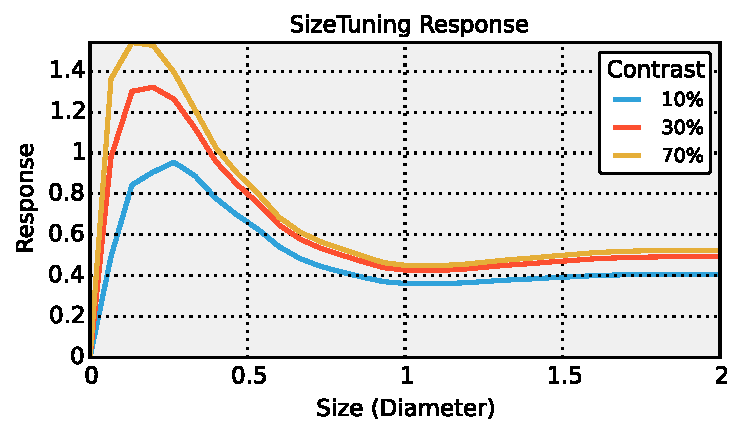
\includegraphics[width=0.5\textwidth]{./results/SCAL/LGN_SizeTuning.pdf}
	\caption[SCAL model size-tuning curves]{LGN neuron size tuning
      representing the response of a stereotyped LGN neuron to a
      sinusoidal grating disk stimulus with increasing contrast. The
      tuning curves demonstrate a small but noticeable shift toward
      larger size preferences at lower contrasts.}
	\label{LGNSizeTuning}
\end{figure}

\begin{figure}
	\centering
        \includegraphics[width=1.0\textwidth]{./results/SCAL/LGN_DoG.pdf}
	    \caption[SCAL model size-tuning DoG
          fit.]{Difference-of-Gaussian model goodness of fit
          comparison for SCAL size-tuning curves. A) LGN
          area-summation curve (gray) fitted using a subtractive
          (blue) and divisive (red) integrated DoG model. B) Fraction
          of explained variance ($R^2$) of the subtractive and
          divisive DoG models.}
	\label{LGNSizeFit}
\end{figure}

Since LGN responses in this model do not have any source of
variability we cannot compare the distributions directly. To compare
the responses with the experimental results we will treat the 10\%
contrast response as the low contrast response and 70\% contrast as
the high contrast response. This matches the experiment where the
contrast with 20-50\% and 70-90\% of the maximal response are taken as
low- and high-contrast responses respectively. To compare the data
directly to the experimental data, we have overlaid the low and high
contrast estimates of the excitatory and inhibitory constant directly
on experimental data from \cite{Sceniak2006} (see
Figure~\ref{LGNDistribution}).

The excitatory space constant $a$ was estimated at $0.16\degree$ at
high contrast, expanding to $0.294\degree$ at low contrast. The
inhibitory or surround space constant on the other hand was
$0.62\degree$ at low contrast and $0.56\degree$ at high contrast.
These values fall well in the distributions that have been measured in
experiments, even if they are reaching toward the smaller end of what
was measured in thalamocortical afferents in the visual cortex.

\begin{figure}
	\centering   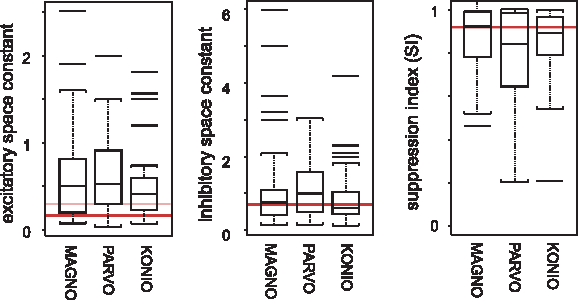
\includegraphics[width=1.0\textwidth]{./Sceniak_LGN_Distribution.pdf}
	\caption[Distribution of excitatory and inhibitory in
      thalamocortical afferents.]{Distribution of excitatory and
      inhibitory space constants in thalamocortical afferents
      reproduced from \cite{Sceniak2006} (in macaque) and overlaid
      with estimates obtained from the SCAL LGN model at low contrast
      (pink) and high contrast (dark red).}
	\label{LGNDistribution}
\end{figure}

\subsubsection*{Frequency Tuning}

The frequency tuning of LGN neurons in macaque V1 is strongly
correlated with the size tuning, nonetheless we want to confirm the
frequency tuning curve matches what is seen in experiment. Therefore
we replicate the frequency tuning measurements performed by
\cite{Levitt2001}. The sinusoidal gratings used for measurement were
presented in a $2x2^{\circ}$ area, well beyond the size of the
surround field. The resulting frequency tuning curves are shown in
Figure~\ref{LGNFrequencyTuning}, largely displaying contrast
invariance.

\begin{figure}
	\centering
    \includegraphics[width=0.5\textwidth]{./results/SCAL/LGN_FrequencyTuning.pdf}
	\caption{LGN neuron frequency tuning representing the response of
      a stereotyped LGN neuron to a $2x2^{\circ}$ sinusoidal grating
      stimulus at a wide range of contrasts.}
	\label{LGNFrequencyTuning}
\end{figure}

We compare the spatial frequency preference of the model LGN directly
with a scatter plot of spatial frequency preferences against
eccentricities, again demonstrating that we are well within the
empirically validated distribution of values (see
Figure~\ref{LGNFrequencyLevitt}).

\begin{figure}
	\centering
    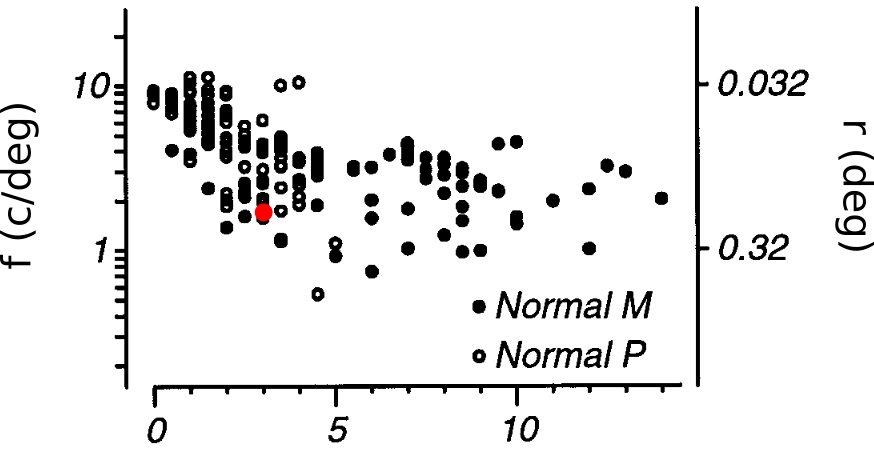
\includegraphics[width=0.8\textwidth]{./LGN_FrequencyLevitt.png}
	\caption[Spatial frequency preference in SCAL compared to
      experiment. Adapted from \cite{Levitt2001}.]{Plot of preferred
      frequency tuning of neurons in the LGN of normally reared and
      visually deprived macaque monkeys overlaid with the optimal
      spatial frequency of the stereotyped SCAL LGN neuron (red
      circle). Preferred spatial frequency is within the range of
      preferred spatial frequencies and is well adapted to provide
      appropriate input for the V1 models. Adapted from
      \cite{Levitt2001}.}
	\label{LGNFrequencyLevitt}
\end{figure}

\subsection{The V1 model}

Before going into the spatial calibration of the V1 stage of SCAL
model, we will first review how the model self-organizes into a
smooth, high-quality orientation map. The model was in most cases
simulated as a $4^\circ x 4^\circ$ area, which corresponds to around
$12 mm^2$ of cortical area. After training a wide range of
measurements were performed to confirm the model developed correctly
and exhibited the same properties as GCAL.

The orientation map, receptive fields and orientation tuning curve for
the fully developed model are shown in
Figure~\ref{SCALORTuning}. These results demonstrate that the final
spatially calibrated model still exhibit good quality orientation
maps, contrast independent orientation tuning and very clear oriented
lobes in individual receptive fields. Comparing the robustness of map
organization to the GCAL model will be performed later on, when we are
looking at the properties that make a model robust to a wide range of
inputs.

\begin{figure}
  \begin{minipage}[t]{0.67\textwidth}
    \mbox{}\\[-\baselineskip]
    \includegraphics[width=\textwidth]{./results/SCAL/SCAL_V1_ORTuning.pdf}
  \end{minipage}\hfill
  \begin{minipage}[t]{0.3\textwidth}
    \mbox{}\\[-\baselineskip]
    \caption[Orientation tuning properties of the SCAL model.]{SCAL
      model orientation tuning properties after presenting 20,000
      oriented Gaussian patterns. A) Orientation map measured by
      presenting sine gratings at the optimal spatial frequency to the
      model, along with the locations of the receptive fields shown in
      B. B) Gabor fits to receptive fields measured using sparse
      random noise. C) Orientation tuning curve of a single neuron
      across contrasts, demonstrating largely contrast-independent
      orientation tuning. The model exhibits some diversity in tuning
      properties with different tuning bandwidths and even very
      broadly tuned neurons.}
    \label{SCALORTuning}
  \end{minipage}
\end{figure}

Additionally, to get a better understanding of how the model processes
visual inputs in a single presentation and over development, we have
plotted the response of the neurons to a simple Gaussian pattern drawn
on the retina before and after development in \ref{SCALResponse}. The
figure highlights how the model initially responds with a diffuse
activity pattern driven, while forming so called activity bubbles
corresponding to individual orientation columns after development.

\begin{figure}
	\centering
    \includegraphics[width=1.0\textwidth]{./results/SCAL/SCAL_Response.pdf}
	\caption[SCAL Responses to a simple Gaussian pattern before and
      after self-organization.]{SCAL Responses to a simple Gaussian
      pattern before and after self-organization. Top left shows the
      input pattern and the LGN ON/OFF response to the pattern. Top
      right shows the evolving patterns of activity before and after
      development. The response of the central neuron at various
      stages of development is shown at the bottom. Demonstrates
      initial randomness of connections, the process of settling, and
      finally a selective response reflecting the process of
      self-organization. }
	\label{SCALResponse}
\end{figure}

\subsection{V1 Spatial Calibration}

A neuron in primary visual cortex receives input from a variety of
sources, including feedforward connections from the LGN, horizontal
connections from within V1 and feedback connections from extrastriate
cortex as seen in Figure~\ref{RFstruct}. Translating the fully
complexity of the known spatial profiles of these different synaptic
inputs to the visual cortex therefore requires integrating a wide
range of information from different sources including anatomical,
electrophysiological and optical imaging. Not only will this let us
build a model that corresponds more closely to the macaque visual
cortex in vivo, but also let's us cross-validate the experimental
data, highlighting potential discrepancies.

The first step to bridge measurements from different sources will be
to establish a well defined mapping from visual space to cortical
space. From there we will evaluate the different sources of
measurement, replicating the measurements in the model and comparing
the results. Finally we will summarize the model parameters that were
chosen and will be carried over to later models.

\subsubsection*{Magnification factors \& Hypercolumn Distance} \label{SCALHypercolumns}

As we outlined above most studies of V1 particularly in the surround
modulation literature focus on parafoveal regions between $2-5\degree$
in eccentricity. Therefore we have chosen to model the region around
$3\degree$ in eccentricity. This already gives us a number of
constraints, first of all giving us an approximate V1 magnification
factor of 3 mm/\degree as described by \cite{VanEssen1984} and shown
in Table~\ref{MFs}. This means that each degree of visual space
corresponds to 3 mm on the cortical surface at this particular
eccentricity. However without an independent measure of the cortical
space this conversion factor is still entirely arbitrary. Therefore we
make use of the fact that the hypercolumn distance between orientation
columns in V1 is well defined by numerous studies.

% jbednar: would be more readable if the citations would fit into the
% first column; seems like they might
\begin{table}
\centering
\begin{tabular}{l | c c}
  \hline
  \hline
  Visual Area     & Magnification Factor ($mm/\degree$) & Anisotropy Index \\
  \hline
  Retina$^1$      & 0.223                            & -                      \\
  LGN$^2$         & 0.324                             & 1.0-2.0                \\
  V1$^3$          & 2.54-3.545                       & 1.0-3.0                \\
  \hline
\end{tabular}
\caption[]%
{Magnification Factors and Anisotropy Index associated with different
  visual areas at $3\degree$ eccentricity estimated from areal and
  linear magnification factor equations. Footnotes: $^1$ -
  \cite{Perry1985}, $^2$ - \cite{Connolly1984}, $^3$ -
  \cite{VanEssen1984}}
\label{MFs}
\end{table}

To give actual scale to our model, we can therefore measure the
orientation map hypercolumn distance. Using estimates provided by the
Wolf group the hypercolumn distance in macaque V1 has been estimated
at roughly ($710 \pm 50 \mu m$). By combining this information with
the magnification factor, we can establish that we would expect
roughly 4.2 hypercolumns per visual degree ($3 mm/\degree \cdot 710
\mu m$). We will also define an acceptable range of hypercolumn cycles
per degree to ensure later models do not diverge too far from the
spatial tuning implemented here. Taking the confidence intervals for
both the magnification factor and hypercolumn distance into account
the acceptable range of hypercolumns per sheet coordinate is between
3.29 and 5.3.

The hypercolumn distance in the model was calculated by taking the 2D
Fourier transform of the orientation map, reducing it to one dimension
and applying a least-squares fit of a Gaussian curve with additional
linear and quadratic terms (see \cite{Kaschube2010} for more
details). A sample fit to an SCAL orientation map can be seen in
Figure~\ref{SCALhypercolumns}. The final model has ~3.86 hypercolumns
per visual degree, which falls well within the allowed range. Models
trained on natural images not shown here, generally fall in the range
of 4-4.5 hypercolumns per visual degree.

Based on that measurement we can now explicitly state that 1 visual
degree corresponds to 3 mm in the model, which will let us
independently confirm that the extent of the final model weights are
consistent with experimental measurements but also internally
consistent with the size-tuning response of the model. The next steps
will be to evaluate feedforward and lateral connections independently.

% jbednar: I guess the table can't use Greek letters (latex equations)
% natively?
\begin{figure}
	\centering
        \includegraphics[width=1.0\textwidth]{./results/SCAL/PinwheelAnalysis.pdf}
	\caption[Hypercolumn and pinwheel density fitting procedure and
      results.]{Hypercolumn and pinwheel density fitting procedure. A)
      Orientation map in V1 overlaid with real and imaginary contours
      and pinwheels at their intersections. B) 2D FFT of the
      orientation map showing a ring identifying the periodicity of
      the map. C) 1D histogram of the FFT along with Gaussian fit
      marking the best fit hypercolumn distance. D) Summary table
      showing various parameters of the fit, along with pinwheel
      density ($\rho$) which classifies the quality of the map. The
      SCAL model exhibits near $\pi$ pinwheel density a measure that
      has been associated with realistic orientation maps
      \citep{Kaschube2010, Stevens2013b}.}
	\label{SCALhypercolumns}
\end{figure}

\subsubsection*{Feedforward}

The afferent input from the lateral geniculate nucleus is the main
driver of responses in the primary visual cortex. It is therefore
crucial in determining the size-tuning profile of the visual cortex.
In section \ref{AfferentBackground} we discussed how the integrative
area of a neuron in V1 is made up of the combined integrative area of
thalamocortical projections and retinogeniculate projections.

\paragraph{Area summation}

The first step in the fitting procedure was to repeat the protocols
applied to the LGN, i.e. measuring area summation curves and fitting
DoG models to the results. Using this approach we obtained a large
number of size estimates for the excitatory and inhibitory kernels
contributing to the V1 response, which we can compare to the results
obtained from comparable studies in macaque visual cortex.

\begin{table}
  \centering
  \begin{adjustbox}{width=1\textwidth}
  \begin{tabular}{l | l l l l}
    Measurement              & Literature            & Layer & Diameter \\
    \hline
    V1 hsRF                  & \cite{Levitt2002}     & 2-6 & $1.0 \pm 0.1\degree$ (0.15 - 1.1) \\
    \hline
    V1 Excitatory DoG fit    & \cite{Levitt2002}     & 2-6 & $0.9\degree$ \\
                             & \cite{Sceniak2001}    & 2-6 & $2.0\degree$ \\
                             & \cite{Cavanaugh2002}  & 2-6 & $1.4\degree$ \\
                             & \cite{Solomon2002}    & not stated & $0.94\degree$ \\
    \hline
    V1 Inhibitory DoG fit    & \cite{Levitt2002}     & 2-6 & $1.9\degree$ \\
                             & \cite{Sceniak2001}    & 2-6 & $4.4\degree$ \\
                             & \cite{Cavanaugh2002}  & 2-6 & $2.7\degree$ \\
                             & \cite{Solomon2002}    & not stated & $2.97\degree$ \\
    \hline
  \end{tabular}
  \end{adjustbox}
  \caption[Functional estimates of V1 receptive field size using
    Difference-of-Gaussian models.]{Functional estimates of V1
    receptive field size using Difference-of-Gaussian
    models. Measurements differ due to measurement protocols used. All
    measurements come from macaque V1.}
  \label{electrophystable}
\end{table}

The Table~\ref{electrophystable} summarizes the mean results obtained
by these studies, with a general agreement of an afferent integration
field that spans about $1\degree$ in diameter, with inhibitory
surround that is on average about two times larger at about
$2\degree$. The most thorough analysis being performed by
\cite{Cavanaugh2002}, who fitted a number of variants of the model. In
addition to measuring integrative area of V1 neurons in visual space
they converted the results into cortical space using the known
magnification factor. In Figure~\ref{CavanaughDistribution} the
results from the model, also converted to cortical space are compared
to these distributions, showing less diversity but general agreement
on mean and median values.

\begin{figure}
	\centering
        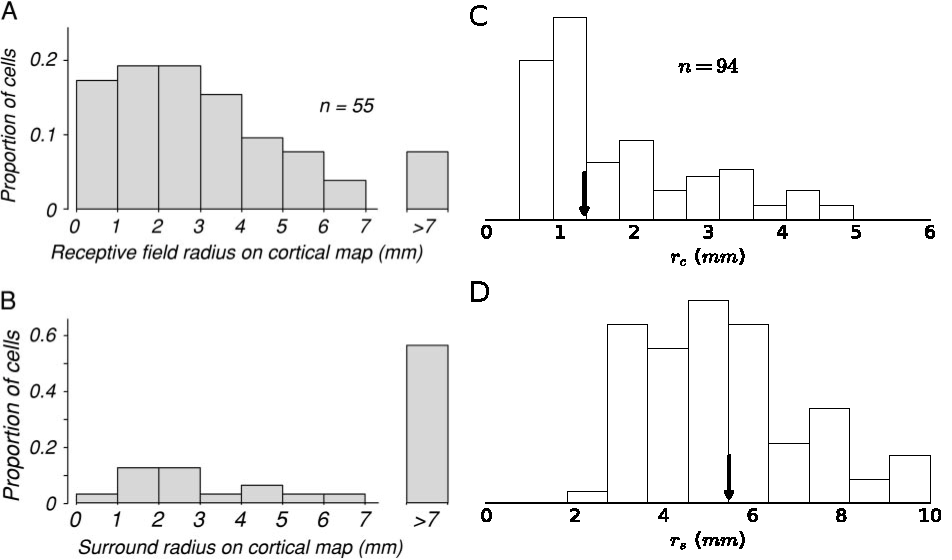
\includegraphics[width=1.0\textwidth]{Cavanaugh_V1_Distributions.pdf}
	\caption[Distribution of V1 Difference-of-Gaussian space constants
      measured by \cite{Cavanaugh2002} compared to SCAL
      model.]{Comparison between the distributions of space constants
      estimated by \cite{Cavanaugh2002}, converted from visual angle
      to cortical space and the equivalent measurements applied to the
      model. A, C) Distributions of maximal integration area radii.
      B, D) Distributions of suppressive surround area radii. }
	\label{CavanaughDistribution}
\end{figure}

Additionally we also compare the shift in size-tuning preference
between low and high contrast conditions, between experiment
\citep{Sceniak1999} and the model. In addition to the SCAL model, the
analysis also includes results from GCAL, which employs subtractive
rather than divisive inhibition. The results highlight that the GCAL
model does not really exhibit any meaningful size-tuning shift between
low and high contrast. Additionally both model scatter plots clearly
highlight the lack of diversity in the model. Generally however, the
results are qualitatively very similar between SCAL and the
experimental data, showing a mean shift and distribution of shifts
that is very similar (2.2x shift in experiment vs. 1.8x in the model).

\begin{figure}
	\centering
        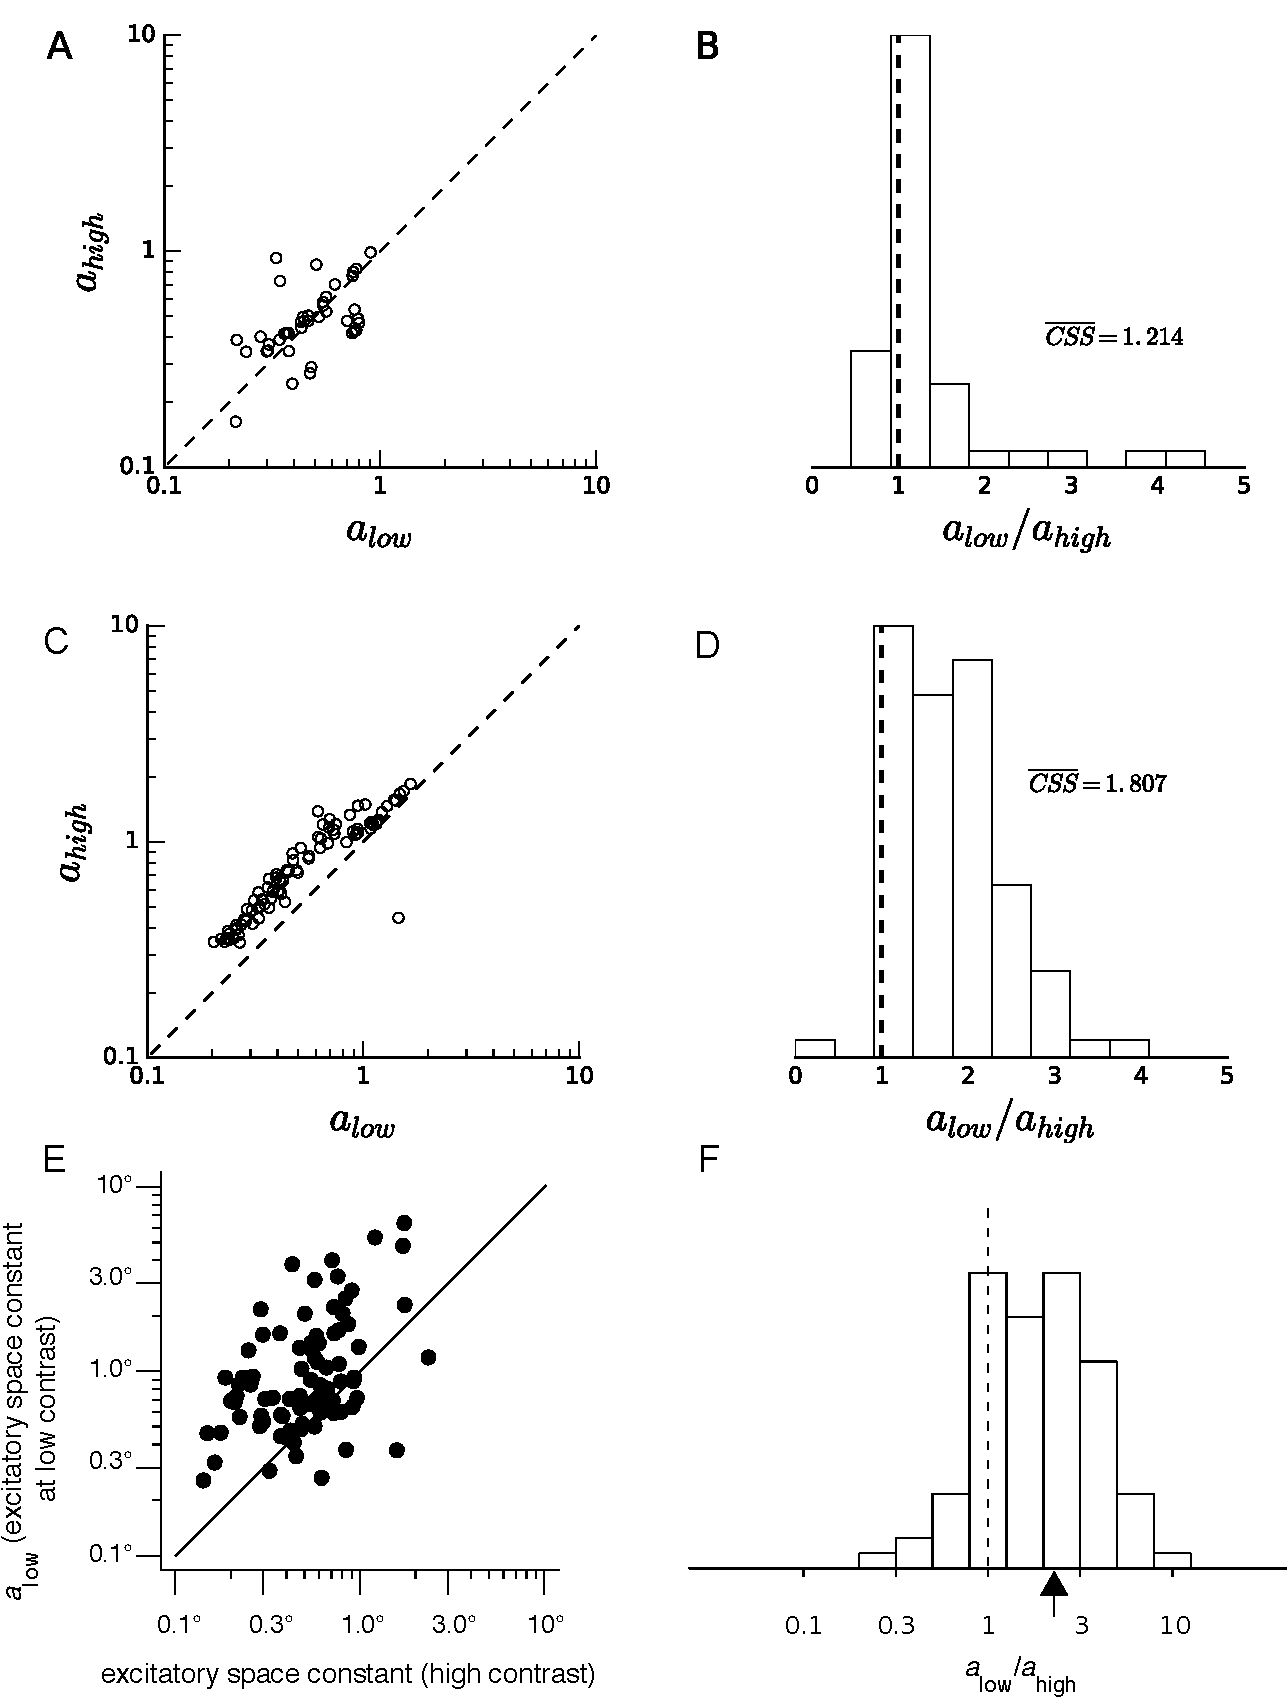
\includegraphics[width=0.8\textwidth]{./V1_DoG_Contrast.pdf}
	\caption[Contrast-dependent size-tuning shifts compared between
      GCAL, SCAL and experimental results from
      \cite{Sceniak1999}.]{Comparison between contrast-dependent
      size-tuning shifts between the GCAL model (A, B), the SCAL model
      (C, D) and experimental results from \cite{Sceniak1999} (E,
      F). A, C, E) Scatter plot of DoG excitatory constant at low and
      high contrast in experiment and the model respectively. B, D, F)
      Distribution of contrast-dependent shift in excitatory
      constant. The introduction of divisive gain control results in a
      significant contrast-dependent size-tunign shift.}
	\label{ContrastShift}
\end{figure}

Finally we investigate the distribution of suppression indices, which
shows a similar mean value but also highlights the complete lack of
unsuppressed cells.

\begin{figure}
	\centering
        \includegraphics[width=0.6\textwidth]{./results/SCAL/SCAL_V1_SI.pdf}
	\caption{Distribution of Suppression Index (SI) values under
      high-contrast stimulus condition.}
	\label{SCALSI}
\end{figure}


\paragraph{Receptive Fields}

In addition to measuring the area summation responses of V1 neurons we
can also assess the spatial profile of V1 receptive fields by mapping
them using reverse correlation techniques. After mapping the receptive
fields using 5000 sparse, random stimuli the results were fit using
the simple Gabor model described in Section~\ref{rffitting}. In
addition to once again confirming the spatial frequency preference of
the neurons, we compared the $n_x$ and $n_y$ ratios of the neurons to
equivalent measurements in macaque \citep{Ringach2002b} and cat
\citep{Jones1987}.

The results show a similar general shape but also demonstrate a shift
toward greater $n_x$ values as compared to the experimental data.

\begin{figure}
	\centering
        \includegraphics[width=1.0\textwidth]{./results/SCAL/RF_nxny.pdf}
	\caption[Relative elongation and width of V1 receptive fields. A
      comparison between SCAL, cat V1 \cite{Jones1987} and macaque V1
      \cite{Ringach2002b}.]{Scatter plot of receptive field $n_x$ and
      $n_y$ values, representing the width and length of the receptive
      field relative to the period of the grating underlying the Gabor
      fit respectively. Comparison between results from
      \cite{Ringach2002b} in macaque V1 (circles), \cite{Jones1987} in
      cat V1 (crosses) and in the SCAL model (squares).}
	\label{RFFits}
\end{figure}

\subsubsection*{Intracortical connectivity}

We have already settled that afferent activity is the major driver of
responses in primary visual cortex but intracortical, recurrent
connections between neurons are though to provide significant
modulatory influences on V1 responses. Precisely breaking down the
contributions of specific connections, particularly when taking into
account the cell types is much more difficult, particularly because
experimental data is much more scarce. In
Section~\ref{InhibitoryBackground} we summarized the potential role of
different inhibitory subclasses, however beyond some estimates of the
maximum extent of the axonal projections from different cell classes
\citep{Kisvarday1993, Kisvarday1997a, Budd2001, Buzas2001}, very
little is known about their spatial profile. The extent of excitatory
projections between V1 neurons are better studied, with a range of
estimates for the maximum extents \citep{Angelucci2002} and even some
models of the spatial profile of connections \citep{Buzas2006} being
available.

We summarize various anatomical estimates of the extents and spatial
distribution of intracortical connections in
Table~\ref{anatomicaltable}. Note that due to the lack of data a lot
of these estimates were obtained in cat V1, which means we have to
extrapolate these results to macaque V1.

\begin{table}
  \centering
  \begin{adjustbox}{width=1\textwidth}
  \begin{tabular}{l | l l l l}
    Connection               & Literature            & Species & Layer & Diameter \\
    \hline
    LGN-V1 Afferents         & \cite{Angelucci2002c} & macaque & 4C$\alpha$ & $0.8-1.6\degree$ \\
                             & \cite{Angelucci2006a} & macaque & 4A/4C$\beta$ & $0.91 \pm 0.041\degree$ \\
    \hline
    V1 local excitation      & \cite{Buzas2006}      & cat      & 2-4 single cell & $288 \mu m$ \\
                             & \cite{Buzas2006}      & cat      & 2-4 population  & $520 \mu m$ \\
    \hline
    V1 basket cells          & \cite{Buzas2001}      & cat      & 2-6 & $0.7-1.9\degree$ \\
                             & \cite{Buzas2001}      & cat      & 2-6 & $0.76-2.6 mm$ \\
    \hline
    V1 long-range excitation & \cite{Angelucci2002}  & macaque  & 2/3 & $6\pm 0.7 mm$ (3-9) \\
                             &                       &          & 4B/4C$\alpha$ & $6.7 \pm 0.7 mm$ (4.7-10) \\
                             &                       &          & population & $2.47 \pm 0.3\degree$ \\
                             & \cite{Buzas2006}      & cat      & 2/3 & $6 mm$ \\
    \hline
  \end{tabular}
  \end{adjustbox}
  \caption{Anatomical estimates of the spatial profiles of V1
    connectivity from macaque and cat.}
  \label{anatomicaltable}
\end{table}


\paragraph{Excitatory Connections}

The literature has had a much harder time of picking apart the
contribution of intracortical and particularly the patchy lateral
connectivity found in V1 so to confirm that these connections have
developed as expected is to compare it to anatomical measurements.
For this purpose we will be fitting a descriptive model, developed by
\cite{Buzas2006} to the lateral connectivity data.

The distance of long-range connectivity varies considerably across
species so using some anatomical estimates from macaque we will
attempt to refine our estimates of the long-range oriented
component. Anatomic data suggests that the spatial spread of lateral
connections can be anywhere between 3-10 mm (on average 6-7 mm) in
total length \citep{Angelucci2002}. Along its principal axis the
visuotopic mono-synaptic spread of V1 horizontal connections has a
mean of \(2.47^\circ\) \(\pm\) \(0.3^\circ\). This falls well within
the range of estimates for the lsRF as published in a number of
studies \citep{Sceniak1999, Sceniak2001, Shushruth2009}, which employed
the iDoG protocol.

\begin{figure}
	\centering
        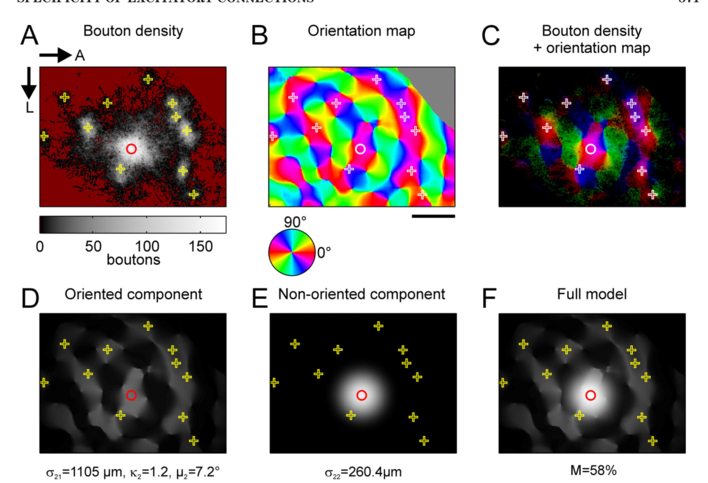
\includegraphics[width=1.0\textwidth]{Buzas.png}
	\caption{Lateral excitatory projection bouton density and
      orientation maps in layer 2/3 of cat V1 demonstrating the
      application of a Gaussian and von Mises model of lateral
      connectivity. Reproduced from \cite{Buzas2006}.}
	\label{Buzas}
\end{figure}

The model that was used to fit the lateral weights describes the
patchy lateral connectivity found in layer 2/3 of V1 as a function of
two distinct components. A short range isotropic Gaussian pattern and
a long range pattern, defined as a von Mises function, which is
combined with the orientation map. The model therefore assumes that
lateral connectivity develops as a function of both the proximity in
space but also along a particular feature dimension, in this case the
orientation. The equations underlying this model and an extension,
which also exposes the aspect ratio of the long-range Gaussian kernel
are described in Section~\ref{BuzasEquations}.

The full model fitting procedure for an experimentally traced lateral
connection field is shown in Figure~\ref{Buzas}. By applying this
fitting procedure we can effectively estimate the spatial extents of
both the local isotropic local kernel and the long-range excitatory
kernel. The Figure~\ref{LatFits} demonstrates what one such fit looks
like for the SCAL model, while the full distribution of local and
long-range kernel values is shown in Figure~\ref{LatDist}. Note that
the weight array that is being fit has been thresholded at the 70th
percentile of non-zero values to ensure the weight matrix more closely
resembles the bouton density maps obtained by \cite{Buzas2006}.

\begin{figure}
	\centering
        \includegraphics[width=1.0\textwidth]{./results/SCAL/SCAL_vonMises_Fits.pdf}
	\caption[Combined Gaussian+vonMises model fits to lateral
      connectivity of the SCAL model.]{Example fits obtained by
      fitting Gaussian and von Mises distributions to the thresholded
      long-range lateral weights. A) The thresholded long-range
      lateral weight matrix (at the 70th percentile). B, C) Example
      fits using the von Mises orientation model with and without an
      aspect parameter. D, E) Error between the fits and the
      thresholded weight matrix pattern.}
	\label{LatFits}
\end{figure}

The results of our fitting procedure shown in Figure~\ref{LatDist}
show good correspondence with these experimental estimates with a mean
long-range connectivity that has a spatial constant of around $1645
\mu m$ but extends beyond that with our cut-off defined at
$2.5\degree$ or $7.5 mm$. The model without aspect fits the
experimentally obtained long-range spatial constant more closely but
neither extends to the furthest reaches of the lateral connection
field. The local excitatory kernel provides a reasonable fit to
experimental estimates with a mean local excitatory kernel with a
spatial constant of around $221 \mu m$, compared to the $280 \mu m$
estimated in cat V1 \citep{Buzas2006}. However most neurons exhibit
much smaller local kernels and the distribution seems to be
distributed bi-modally.

\begin{figure}
	\centering
        \includegraphics[width=1.0\textwidth]{./results/SCAL/SCAL_Buzas_Distributions.pdf}
	\caption[Distribution of spatial constants obtained by fitting
      Gaussian and vonMises model.]{Distribution of spatial constant
      obtained by fitting the \cite{Buzas2006} von Mises and Gaussian
      model to long-range lateral excitatory connections developed as
      part of the SCAL model. A) Distribution of kernel sizes of the
      local excitatory component. B) Distribution of kernel sizes of
      the long-range excitatory component C) Comparison between naive
      model with orientation dependent component (i.e. pure Gaussian),
      the vonMises model including the orientation dependent component
      and additionally versions of both with an additional term for
      the anisotropy in the connectivity.}
	\label{LatDist}
\end{figure}

Finally we can evaluate in how far the orientation preference and
selectivity of the post-synaptic neuron predicts the long-range
lateral connections it receives. Specifically we can evaluate how
closely the $\kappa$ value of the von Mises fit, which represents the
bandwidth of the kernel in the orientation domain, is correlated with
the orientation selectivity of the neuron. The relationship between
these two variables is shown in Figure~\ref{LatORKappa}, and clearly
predicts that the orientation specificity of the lateral connections
received by a V1 neuron is highly dependent on the orientation
selectivity of the neuron (Spearman's $\rho=0.59$, $p<10^{-184}$).


\begin{figure}
	\centering
        \includegraphics[width=1.0\textwidth]{./results/SCAL/SCAL_vonMises_ORSel.pdf}
	\caption[Relationship between the width of vonMises distribution
      in the lateral connectivity model and the orientation
      selectivity of the neuron.]{Scatter plot of the $\kappa$
      variable of the von Mises distribution and the orientation
      selectivity of each neuron, showing a clear relationship between
      the orientation specificity of patchy lateral connections and
      the post-synaptic neurons orientation selectivity. The points
      are additionally colored by their goodness of fit and marginal
      histograms of the distributions of the $\kappa$ and orientation
      selectivity are provided. Fits with an $R^2$ value below 0.3
      were rejected.}
	\label{LatORKappa}
\end{figure}

\subsubsection*{Inhibitory connectivity}

Since the SCAL model does not have distinct populations of V1 we will
consider the joint spatial and orientation distribution of basket
cells in order to determine the inhibitory profile and compare model
to experiment. \cite{Kisvarday1997a} provide the best known estimates
for the spatial distribution of inhibitory basket cells, having
injected tracers much more conservatively than previous studies. Their
estimates indicate that inhibitory projection in cat V1 extend no
further than 1.5-2 mm with most synaptic boutons being distributed in
a central regions approximately 1 mm in diameter. In the absence of
any precise fits, equivalent to the Gaussian and von Mises model
available for the excitatory connectivity, we restrict inhibitory
connectivity to a conservative 1.2 mm in diameter, which excludes the
long tail of these connections.

By binning the strength of connections by their distance and the
orientation difference between pre- and post-synaptic neurons we can
at least qualitatively assess how closely the model distribution
matches experimental bouton density maps. The analysis breaks down the
spatial distribution of connections targeting iso-, oblique and
cross-orientation regions, comparing against the equivalent analysis
performed by \cite{Kisvarday1997a} in cat area 17. While we are
restricting the inhibitory connectivity to a smaller region the
experimental results highlight again that most weights fall into the
central region. Additionally we can see that the distributions of
weights broken down by distance are qualitatively very similar, with
most of the weight in the iso-orientation case being centered near the
center, while oblique and cross-orientations are strongest at medium
ranges.

\begin{figure}
	\centering
        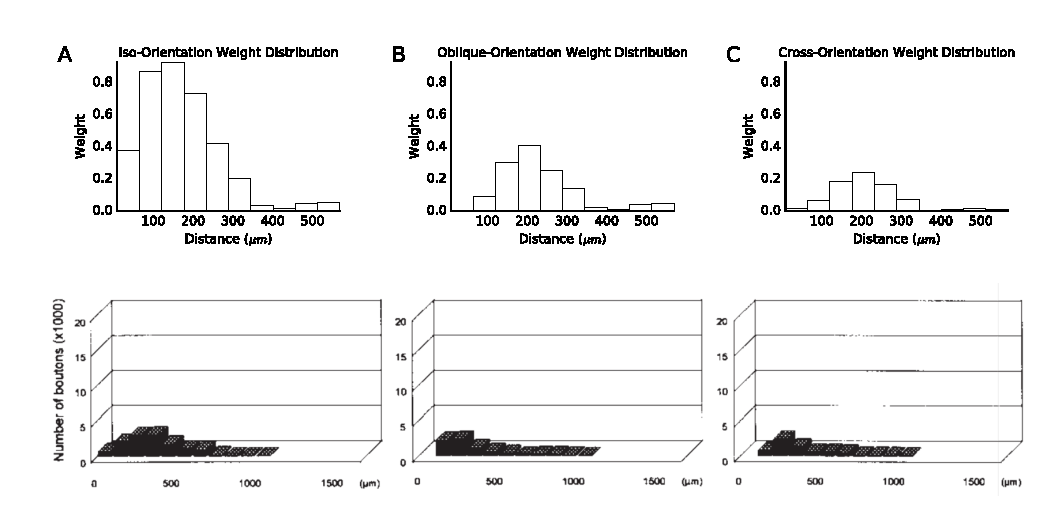
\includegraphics[width=1.0\textwidth]{./SCAL_Inh_Distribution.pdf}
	\caption[Spatial and orientation distribution of the lateral
      inhibitory weights in SCAL.]{Distributions of inhibitory
      projections as a function of space broken down into
      iso-orientation, oblique orientation, and cross orientations
      relative to the orientation preference of the post-synaptic
      neuron. Top row shows model results bottom row reproduces
      results from \cite{Kisvarday1997a} in cat area 17. Comparison
      highlights similarity although the model truncates the heavy
      tail of the distribution.}
	\label{LatORDist}
\end{figure}

\subsubsection*{Sparsity of connections}

The implementation of the GCAL and SCAL models has generally meant
that neurons densely innervate neurons within the defined spatial
extent. However from experimental studies it is known that neurons
actually only make fairly sparse contact to neurons around them and
once the initial sprouting and pruning phase of development is over it
is generally much harder to form new connections. In particular we
know that a V1 neuron is only contacted by a fairly small number of
afferent projections from the LGN and that lateral projections while
very dense innervate only a small fraction of neurons around
them. This has profound implication for development because neurons
have much sparser input than is assumed in these models, secondly it
can strongly affect the development of the model because once
connections have been formed it is much more difficult to shift the
synaptic weights to some other location.

A detailed investigation into the processes underlying sprouting and
pruning and the competition for afferent inputs would be a thesis in
itself. However for computational purposes but also to test the
robustness of the model we implemented a simple form of sprouting and
pruning, which starts out with a densely connected network and slowly
prunes away connections while also generating a small number of new
weights.

In this way we can demonstrate that sparsity of connections can indeed
increase the robustness of the model and that how true long-range
patchy connectivity akin to the thresholded version used in the von
Mises model fitting procedure can emerge from the model.

\section{Discussion}

In this chapter we set out to spatially calibrate the GCAL
developmental model in order to cross-validate known measurements of
the spatial profile of afferent, excitatory and inhibitory connections
in the primary visual cortex. Additionally we wanted to explore how
the intra-areal connectivity in the cortex can give rise to a Mexican
hat like profile, which is thought to underlie the organization of the
cortical neurons into smooth topographic maps, which optimally map
features in the sensory input onto the surface of the cortex.

In the literature review we had established that long-range
connections in the cortex are almost exclusively excitatory. However
the spatial scales involved in mediating Mexican-hat--like connectivity
are well below the long-range excitatory connections, which can often
span many hypercolumns. By incorporating the empirically determined
spatial scales of the model we were able to establish that the
relatively long inhibitory projections originating from the basket cell
population in V1 are sufficient to account for the Mexican hat
profile. At the same time we show that long-range surround suppression
cannot be implemented directly by these projections and must instead by
mediated by a di-synaptic mechanism, via the long-range excitatory
projections.

First we will review how we determined the spatial parameters of the
SCAL model, before critically reviewing the experimental measurements
given in the light of the model results. This will let us highlight
issues with DoG fitting procedures employed to fit area summation
curves in visual cortex and call into questions some conclusions made
about the source of contrast-dependent size-tuning shifts. Finally we
will discuss the model of lateral excitatory connectivity and how the
addition of an aspect parameter can help us quantify the isotropy of
patchy lateral connectivity in a way that can easily be applied to
experiments.

\subsection{The LGN Model}

In spatially calibrating the early stages of the model, roughly
corresponding to the retinal ganglion cell and lateral geniculate
nucleus, we relied mostly on electrophysiological estimates of the
size and area summation curves of the neurons. In doing so we had two
primary aims, first of all since we chose only a single spatial filter
rather than a distribution for computational reasons. Later models can
easily add further diversity to the model by drawing the the spatial
constants of the center-surround filters from a distribution. In the
absence of this diversity we chose a spatial filter size that had to
have several important properties.

The first was that the chosen values should not diverge too far from
the values obtained by fitting a DoG model to area summation
curves. We confirmed this was the case and plotted the results
compared to the empirical data obtained from \cite{Sceniak2006},
finding the values at the lower end of the distribution.

The second constraint was that the spatial frequency preference of the
neurons could not be too low in order to allow V1 neurons to integrate
over at least one cycle of the main spatial frequency preference. This
meant that the preferred spatial frequency of the network should fall
somewhere between 1 and 2 cycles per degree of visual angle. Again we
confirmed this was the case and compared the result to similar results
obtained by \cite{Levitt2001} in the visual cortex of macaques.

The extent of the gain control projection in LGN could not be
experimentally verified as there is little to no data about the
precise anatomical profile of inhibitory neurons in the LGN. Therefore
we chose a value that would provide divisive gain-control over the
span of the receptive field of a single V1 neuron.

The final model parameters are summarized in
Appendix~\ref{Appendix:Parameters} and visualized in
Figure~\ref{LGNDiagram}. In future this model may be extended by
drawing the extent of these afferent connections from a
distribution. For the purposes of this thesis, this level of
calibration is sufficient however and will provide the V1 model with
input that is roughly at the desired spatial scale.

\subsection{The V1 Model}

The V1 model that was introduced in this chapter is able to replicate
a wide range of experimental results and provides a much closer match
to experimental results than the existing GCAL model. In addition to
spatially calibrating the extents of afferent and lateral connections,
the model is also the first developmental model that uses divisive
rather than subtractive inhibition. The divisive model provides a much
better account of size-tuning responses, which shift to larger
integrative areas depending on the contrast, which agrees with a wide
range of existing models. We also showed that the extents of
inhibitory basket cells is sufficient to account for the Mexican hat
profile that has long been used to explain the organization of neurons
into topographic feature maps by pulling together activity locally and
suppressing it in nearby regions, which leads to a smooth mapping of
different feature preferences across the cortical surface.

However, in exploring this model we have also encountered clear
limitations, the most important of which is the lack of distinct
excitatory and inhibitory populations. Apart from directly violating
Dale's law, this poses a serious problem for a developmental model.
This is because Hebbian learning will ensure the strength and spatial
profile of the neural connections is dependent on the response
properties of the neuron and different cell types may respond very
differently. This has made it difficult to directly compare the
lateral connectivity in the model to experimental data.

\subsubsection*{Differences to GCAL}

There are a number of major changes between the GCAL model and the
SCAL model that was introduced in this chapter. As we have already
emphasized the SCAL model operates on divisive rather than subtractive
inhibition. While inhibition in the brain generally has both divisive
and subtractive effects, the divisive normalization paradigm has shown
tremendous success in explaining a wide range of effects including
modulatory effects, contrast-dependent changes in responses,
decorrelating the inputs and even effects associated with visual
attention \citep{Cavanaugh2002a, Graham2011, Carandini2012,
  Reynaud2012, Coen2015}.

The other aim was to move away from other unrealistic
mechanisms. While the model does not learn continuously it no longer
artificially resets the activity between stimulus presentations or
saccades. The model now behaves more continuously with no hard reset
between stimulus presentations. Instead the model activity from a
previous step decays at the start of a new presentation and is usually
extinguished completely by the time it reaches V1.

While all the spatial profiles have changed in some way or another the
most significant change was the size of the afferent field relative to
the lateral connections in V1. While the receptive fields of neurons
in GCAL generally only subtended only a single hypercolumn, the
receptive fields in SCAL span somewhere between 3-4
hypercolumns. Long-range connectivity in the GCAL model therefore
generally connected neurons with non-overlapping receptive fields,
while the SCAL model highlights that this is generally not the case in
parafoveal regions of macaque V1. A good portion of the lateral
connectivity field actually connects neurons with significantly
overlapping connection fields and only a portion of long-range patchy
connections reaches outside the neurons receptive field. This has
significant implications for the function of these connections, rather
than purely reflecting the co-occurence of stimuli the patchy
connections will strongly mirror the response of the neuron
itself. This suggests that lateral connections are involved in
improving the encoding of the local stimulus in addition to mediating
true surround influences.

Despite some of these limitations the model exhibits very robust
development under varying stimulus conditions and still exhibits all
the nice properties of the GCAL model, including contrast invariant
orientation tuning as well as robust, yet adaptive self-organization.

\subsubsection*{Size tuning}

A major component of the analysis we applied here was in comparing
applying a Difference-of-Gaussian model to the area summation curves
and comparing the results to equivalent experimental data. Since the
model itself does not exert any long-range influences any changes in
the fit is must likely mediated by the relatively short-range
connections in the model. However we did find significant shifts in
the integration area depending on the contrast level in the SCAL model
but not in the GCAL model. This suggests suggest the 
contrast-dependent shifts in effective integration area can be explained by
changes in the relative gain of the center and surround component in a
ratio-of-Gaussians model, just as was proposed by
\cite{Cavanaugh2002}. It is therefore not necessary to invoke
integration over a larger area via long-range lateral connections as
was suggested by the experimental work by \cite{Levitt2002} and
\cite{Sceniak2001} and translated into a model by
\cite{Schwabe2006}. This does not mean however that long-range lateral
connections do not have any influence. Indeed it is difficult to
envision how the model can mediate any longer range feature specific
excitation and inhibition without corresponding long-range projections
between neurons, which are themselves tuned for those specific
features.

\subsubsection*{Lateral Connectivity}

\paragraph{Excitatory}

In addition to fitting the response properties of the V1 neurons this
chapter also demonstrated how the anatomical distribution of synaptic
boutons can be compared to the lateral connectivity in the model. By
fitting a model made up of a local Gaussian kernel and an orientation
dependent long-range kernel, first devised by \cite{Buzas2006}, to the
data, we are able to achieve good fits demonstrating that the lateral
connectivity captures the statistics of the visual input. In addition
the results indicated that at least the extent of the long-range
connectivity is consistent with experimental results. However, the
short-range kernels were significantly smaller in scale than what we
would expect from experiment. There are multiple factors that could
account for this difference. The main issue being that the model only
captures one population of cells, which generally display a high level
of feature selectivity. More diversity, such as the introduction of
unselective inhibitory cells could explain larger and more weakly
tuned local connections. Another factor that could play a role is that
neurons in macaque V1 are generally much more dense and the
hypercolumn distance considerably shorter. With relatively larger
hypercolumns we could also expect that the excitatory connectivity
grows in size. Finally, the development of connectivity in the model
is driven entirely by Hebbian rules, and therefore cannot account for
any intrinsic, genetically mediated programming, which could lead to a
dense local network of connections.

We will revisit some of these issues in later chapters to investigate
if some of these factors can significantly affect these results and
whether we can reach a more harmonious fit of the local excitatory
connectivity.

\paragraph{Inhibitory}

The literature surrounding inhibitory connectivity is much more
limited and no detailed estimates of cell-type specific spatial
profiles for the primate visual cortex currently exist. Therefore we
have had to extrapolate from the limited existing data. In the
literature review we explored the known properties of various cell
classes and identified fast-spiking Parvalbumin-expressing
interneurons as the most likely source of connectivity to drive
developmental processes, particularly due to their broad tuning
profile \citep{Albus1994,Kisvarday1997a,Hofer2011,Ma2011} and high
abundance in the thalamocortical recipient layers
\citep{VanBrederode1990,Hogan1992,Huxlin2001} but also because they
have been implicated in developmental disruptions
\citep{Fagiolini2004,Hensch2004}.

In a Hebbian learning model lacking distinct excitatory and inhibitory
projections the distribution of the inhibitory connections is
determined by the responses of the joint population. Therefore it is
not possible to directly compare the inhibitory connectivity profile
to any anatomical equivalents. The comparison of the spatial and
orientation distribution of connections does show significant
similarity however, something we will investigate in more detail when
we have a model that actually expresses distinct excitatory and
inhibitory populations.

\subsubsection*{Diversity of responses}

One of the major design decisions in creating this model was to decide
on whether to match the average response of neurons in V1 or to try to
incorporate the huge amount of variability that is observed in the
real cortex. Due to computational tractability issues we have focused
on matching the average response rather than capturing the full level
of detail immediately. This means that the LGN stage filters the
visual input at just one spatial frequency, which severely limits the
variability in receptive field properties. This is particularly
evident when comparing the distribution of spatial constants, the 
size-tuning shifts and indeed the measured receptive fields themselves.

The receptive field Gabor analysis in particular highlights the lack
of diversity in the receptive fields. This is a direct result of the
lack of LGN filter diversity and a better fit may be achieved by
incorporating a wider range of spatial frequency filters at that
level. Additionally the circular bounding region of the model
connection fields will prevent neurons with very elongated receptive
fields from forming.

There are almost infinite sources of variability in the cortex,
including the distributions of different cell classes, variability in
the number and strength of received connections, and the spatial and
frequency preferences of the feedforward filters. Nonetheless the SCAL
model performs well as a first order approximation and will slowly be
refined as we construct more complex models in later chapters.

\section{Conclusions}

In summary, we have presented the first developmental model of
the primary visual cortex that captures the spatial extents of various
connections in the cortex. Unlike previous static models, performing
this calibration and analysis in a developmental model has several major
benefits. Specifically, because we calibrate only the initial profile
of the connectivity the developmental processes themselves provide a
form of validation for the final results. This property has allowed us
to draw several concrete conclusions.

First of all we were able to establish that the network of local
excitatory and inhibitory connections is sufficient to account for the
Mexican hat profile, which drives the organization of cortical neurons
into smooth topographic maps. Indeed the estimates used for the extent
of inhibitory projections was deliberately chosen to be very
conservative to demonstrate that implausibly long-range inhibitory
connections are not needed to drive development of an orientation map.

Secondly we showed that introducing divisive inhibition is sufficient
to account for contrast-dependent changes in the spatial integration
of V1 neurons. Divisive normalization has been described as a
canonical computation performed by the cortex and indeed we are able
to account for contrast-dependent changes in the response of V1
neurons using the divisive model. This fits the findings by
\cite{Carandini2012} and many others and suggests that long-range
lateral connections are not necessary to account for increases in the
integration area at low contrast as has been suggested by some models
\citep{Levitt2002, Schwabe2006}.

Finally we were able to show that the model develops realistic
long-range patchy connectivity that we were able to fit with an
adapted version of the \cite{Buzas2006} model. This provides a
framework to be able to assess in how far the similarity in feature
preferences between pre- and post-synaptic drives strong connectivity
between the two cells. Additionally it provides a way to
quantitatively assess the spatial extent of these connections.

However we have also identified a number of problems with this model,
the most important of which is the violation of Dale's law, which
states that a single neuron can only employ one main neurotransmitter
and therefore not mediate excitatory and inhibitory effects at the
same time. This has profound effects on the final model because the
connectivity is shaped by responses in a Hebbian model. In the
following chapter we will therefore explore how we can separate these
populations and what properties make different inhibitory cell classes
suited towards specific functions such as sparsifying the response,
divisive normalization and feature specific contextual effects.
 %
%!TEX root = ../PhDthesis.tex
\chapter{Exploring the role of inhibition in cortical development}

In the previous chapter we explored the spatially calibrated SCAL
model, establishing how various sources of evidence about the spatial
structure of V1 projections relate to each other. While this model was
able to account for the size-tuning properties of the visual cortex
quite well, it also exhibited two major shortcomings. Most importantly
it highlighted that a model lacking distinct excitatory and inhibitory
populations will not be able to capture the diversity in connectivity
and response profiles that are observed in the mammalian
cortex. Secondly we showed that based on the known lack of truly
long-range inhibitory projections, long-range orientation-specific
suppression must be mediated by a di-synaptic mechanism mediated by
long-range excitatory connectivity.

Additionally, in the literature section we described the known
properties of various inhibitory cell classes and what roles they
might perform. In particular we discovered that PV and SOM-expressing
interneurons exhibit highly distinct response properties and
layer-specific expression patterns. With recent techniques enabling
the targeting of specific neural populations, there is now huge
interest in understanding their role both in development and in
mediating and gating both contextual and attentional modulation
phenomena.

In this chapter we will propose a model that incorporate the distinct
response properties of an excitatory pyramidal cell population and the
Parvalbumin expressing interneuron population, allowing us to make
concrete predictions about their role in development. We will
establish that the fast and linear response of the PV-ir, fast-spiking
interneuron population makes them ideally suited towards controlling
feedforward activity, sparsifying activity and thereby driving map
formation. Additionally we will show that this model exhibits more
robust and stable map formation even in the presence of strong lateral
excitation than the previous model.

Specifically we will assess how the model performs when manipulating
the response properties of the PV population, under varying levels of
contrast and strong lateral excitation. The SOM inhibitory population
will be disregarded we are primarily focused on development of the
orientation map, which is known to occur before lateral connectivity
emerges, which is known to drive the SOM interneurons. This inhibitory
cell class will be revisited in the following chapters.

\section{Methods}

\subsection{The SEPI Model}

The \textbf{S}hort-\textbf{R}ange \textbf{E}xcitation \textbf{P}V
\textbf{Inhibition} (SEPI) model is based on the same principles,
spatial profiles and equations that were described for the SCAL model
in the previous chapter. However, unlike SCAL, the model has a
distinct excitatory and inhibitory V1 population, which both receive
afferent input and are connected to each other recurrently. The
architecture diagram (Figure~\ref{SEPIDiagram}) shows the two sheets
and projections between them. When comparing this against the SCAL
model diagram (Figure~\ref{SCALDiagram}), we can see that the
spatial scales of the retinotopy, which generally indicates poor
orientation map organization various projections are unchanged---they
have simply been split up between the populations.

\begin{figure}
	\centering
        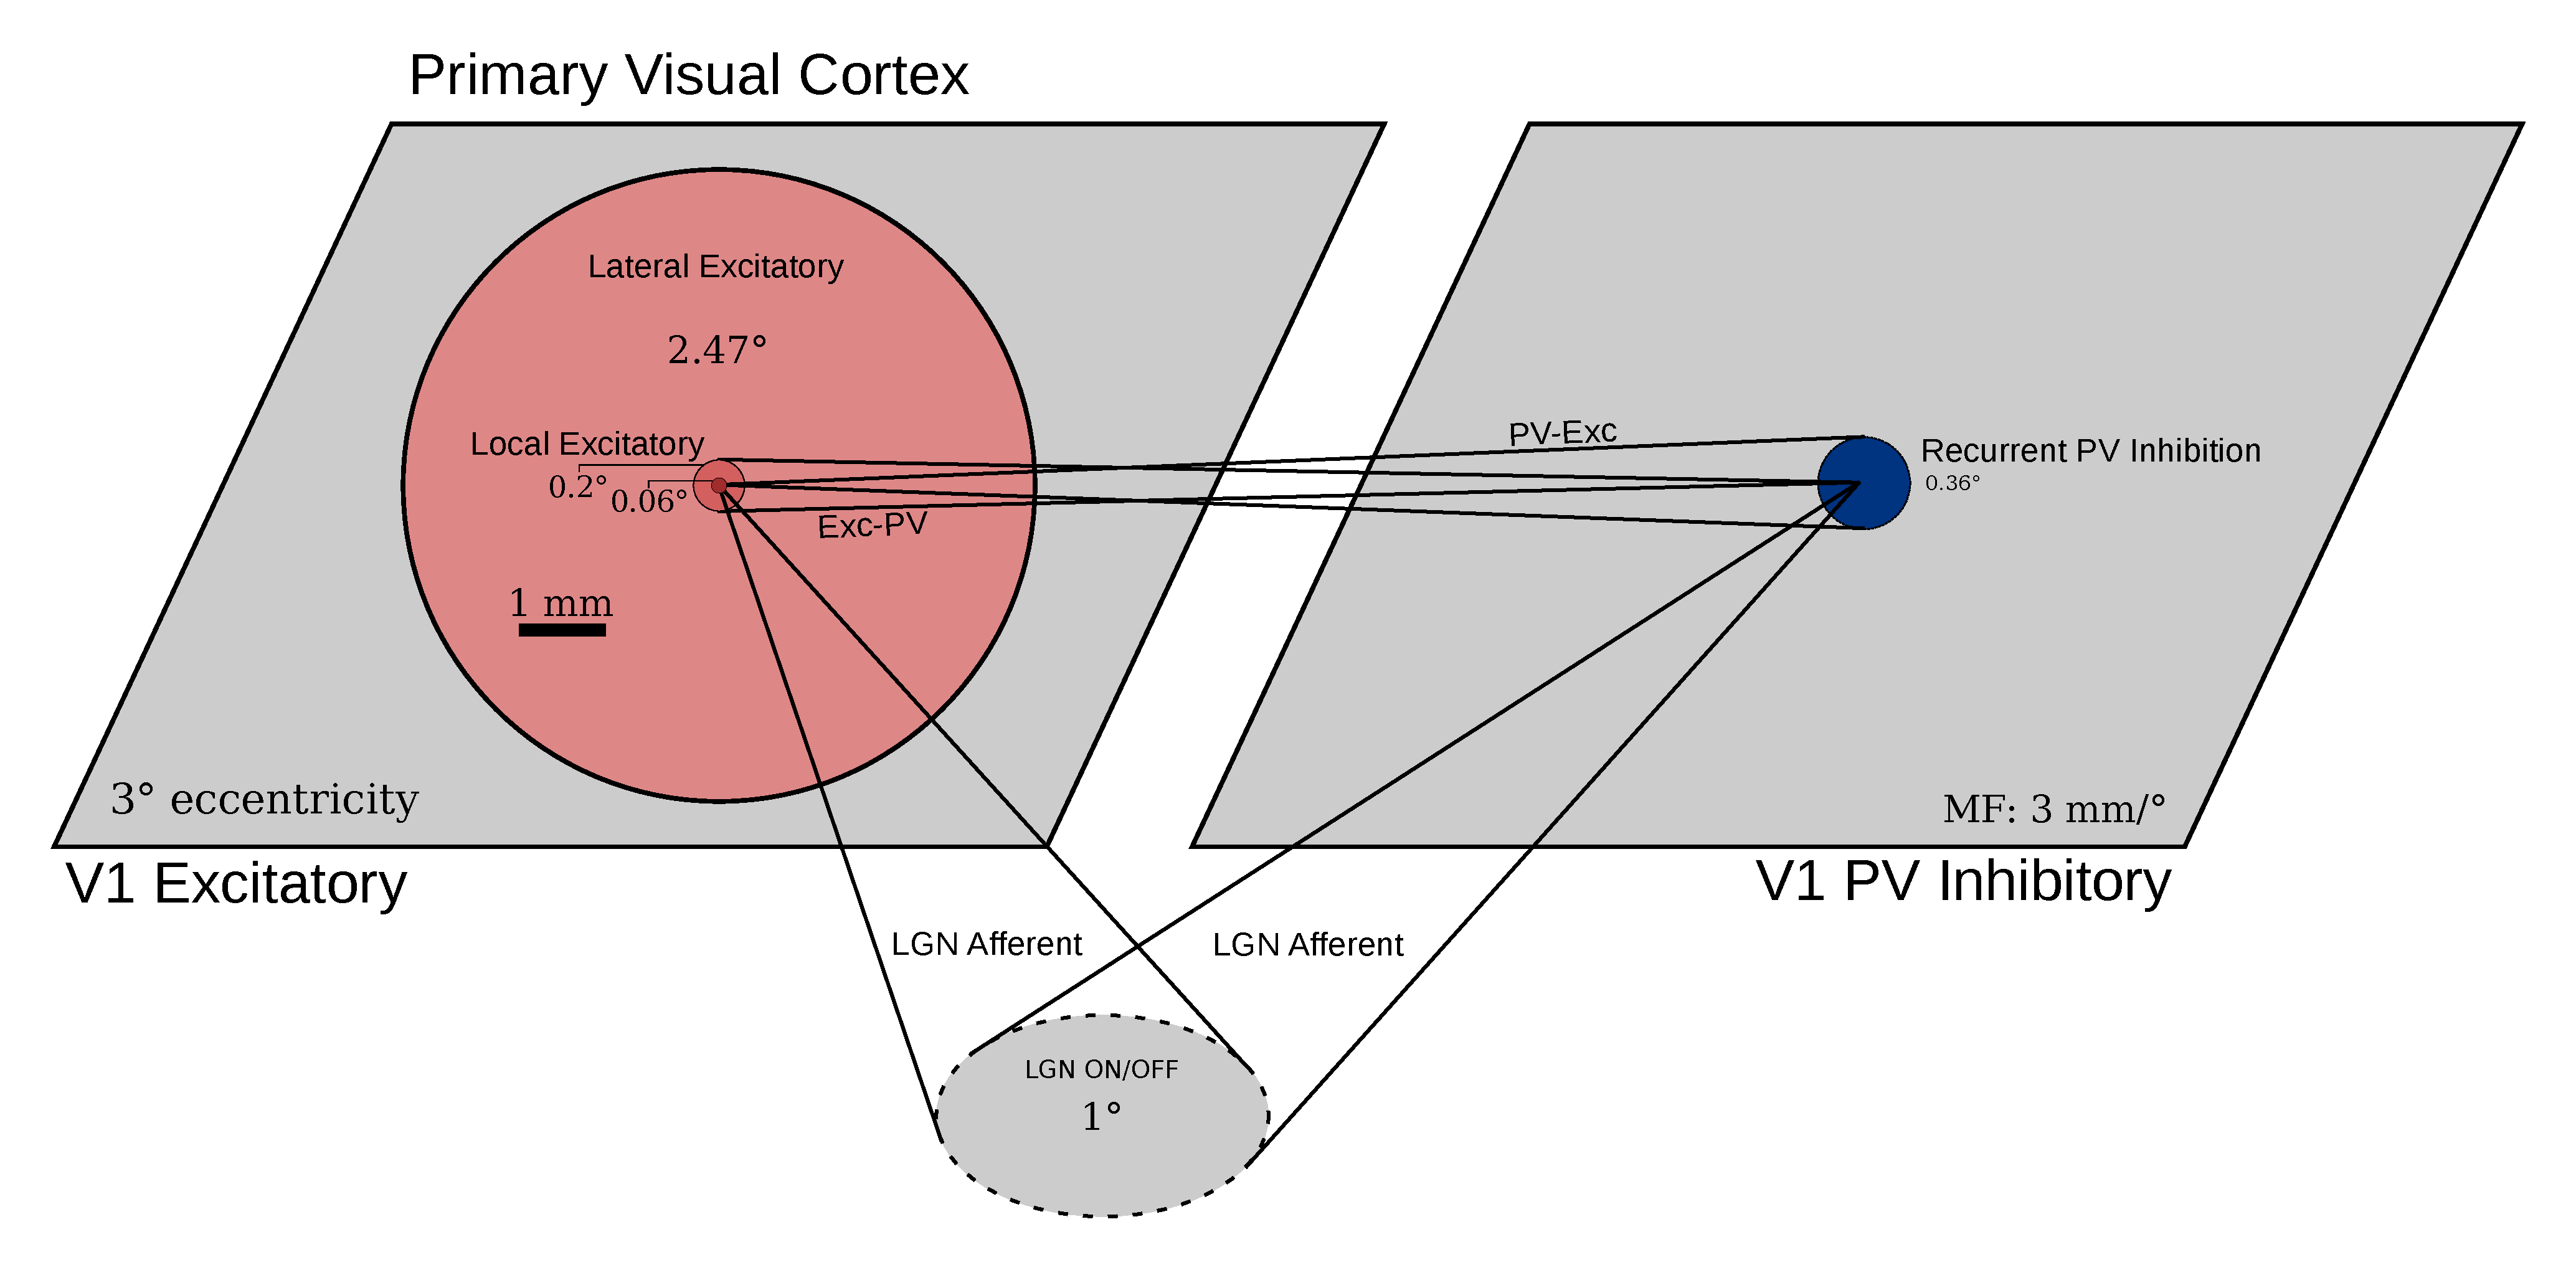
\includegraphics[width=1.0\textwidth]{SEPI_Diagram.pdf}
	\caption{Diagram of the SEPI V1 stage of the model showing the
          spatial scales of the various excitatory (red) and
          inhibitory (blue) connections. Saturated colors indicate the
          kernel radii, while lightly shaded regions indicate kernel
          cut-off extents.}
	\label{SEPIDiagram}
\end{figure}

In the literature review we identified the parvalbumin (PV) expressing
interneurons, which include fast-spiking basket and clutch cells, as
the most likely candidate to provide feedforward inhibition and
controlling the gain of the response in of the pyramidal cells. Their
high abundance in the thalamocortical recipient layer 4 and layers 2/3
(making up over half the population in each;
\citealt{VanBrederode1990}) as well as their involvement in the onset
of the critical period \citep{Fagiolini2000} and their effect on the
columnar organization of the visual cortex \citep{Hensch2004} makes
them of particular interest. The other defining characteristics of the
PV population is their fast response
\citep{Cruikshank2007,Gabernet2005}, and their ability to linearly
match the activity in the excitatory population
\citep{Atallah2012}. These properties describe the role of the
inhibitory projection in the SCAL model, which provides divisive gain
control and is directly coupled to the response of the excitatory
population.

The equations governing the responses of both the excitatory and
inhibitory population are also unchanged, driven by summing the
excitatory input and divided by the inhibitory activity. This closely
matches what we know about PV neurons in the cortex, which provide
strong peri-somatic synaptic inputs to spiny neurons, providing
shunting inhibition \citep{Atallah2012, Wilson2012}. Based on tracing
studies we know that excitatory and inhibitory neurons and
specifically the Parvalbumin expressing subpopulation strongly and
densely innervate each other and themselves \citep{Buzas2001, Ma2011,
  Pfeffer2013}. Additionally these PV population receive strong
afferent input \citep{Burkhalter2008}. All of these properties are
captured by the model.

There is some limited evidence the learning rules on parvalbumin
expressing rules may differ in input cell specific ways with some
anti-Hebbian phenomena having been found in hippocampal circuits
\citep{LeRoux2013}. However for the sake of simplicity the learning
rule applied in the inhibitory population is the same as in the
excitatory population described in equation~\ref{eqn:hebb}.

In order to model the response of the PV population we apply only
half-rectification to the inhibitory population, rather than a
floating homeostatically determined threshold, because basket cells
generally have a very low spiking threshold \citep{Ma2011}.  It would
be possible to use homeostatic plasticity to set the thresholds
instead as suggested by studies in the retina \citep{Hennig2011}, but
it would be complicated to set up mechanisms to balance the thresholds
between the populations to ensure suitable overall levels of activity
in the network. Secondly, we keep the effect of the inhibition
divisive, both for each other and when targeting pyramidal cells.

\subsubsection*{Activation}

The activation for both the excitatory and inhibitory population is
given by:
%%
\begin{equation}
  \eta_E = \eta_I = \frac{\eta_{A} + \eta_{L}}{1 + \eta_{P}}
\label{eqn:sepiactivation}
\end{equation}
%%
where $\eta_{A}$ is the LGN afferent activity, $\eta_{L}$ the local
excitatory contribution and $\eta_{P}$ the PV inhibitory
contribution. In other words, both populations integrate over afferent
and local excitatory input and are then divisively normalized by the
PV population. To allow testing its effects, we will also allow an
optional additional long-range excitation term to modulate the neuron
activity depending on long-range excitatory input:
%%
\begin{equation}
  \eta_{E} = \frac{\eta_{A} + \eta_{L}}{1 + \eta_{P}} (1+\eta_{HE})
\end{equation}
%%
where $\eta_{HE}$ is the input from the horizontal excitatory
projection. The full set of parameters for the SEPI model are list in
Appendix \ref{Appendix:Parameters}. Modeling the long-range input as
an additional multiplicative component has a number of biophysical
explanation, which we will revisit in more detail in the next chapter,
however there is strong evidence that the influence of long-range
excitatory input is strongly voltage dependent \citep{Hirsch1991},
having little effect when afferent input is weak but strongly
modulating the response under stronger input conditions.

The combined activation of the various projections is still combined
in the same way as in the previous models (shown in equation
\ref{eqn:activation1} and as stated above a half-rectifying function
($f$) is used in the inhibitory population, while a homeostatic
function is used among the excitatory population. The response
function of the neurons is therefore given by:

\begin{equation}
\eta_{j,V}(t)=f\left(\frac{\sum_{p=\{E, A\}}\gamma_{p}C_{jp}(t)}{1+\sum_{p=\{I\}}\gamma_{p}C_{jp}(t)}\right)^\beta
\label{eqn:activation2}
\end{equation}

where $\beta$ is the only new term controlling the linearity of the
response, which will be used throughout this chapter.

\subsubsection*{Hysteresis}

In order to control the temporal properties of the PV population we
introduce a hysteresis term, which will be disabled in the final
model but will in the meantime allow us to test the importance of fast
inhibition in the model. The hysteresis function is defined as a discrete
exponential weighting between the previous activation and the new
activity, expressed as:
%%
\begin{equation}
  \eta_h (t + \delta\eta) = \eta(t) + \tau \big[ \eta(t+\delta t) - \eta(t) \big]
\end{equation}
%%
where $\tau$ is the time constant. If $\tau < 1$, hysteresis will
effectively slow down PV responses relative to the excitatory
population. In the final model, the hysteresis term is eliminated simply by
setting $\tau = 1$.

\subsection{Assessing the quality of orientation maps} \label{metrics}

A major component of the analysis applied in this section is to assess
the sensitivity of the model to changes in the response properties of
the different cell classes. Therefore we have to establish a number of
metrics to assess the robustness of the model to changes in contrast
by assessing the quality of orientation map organization.  To measure
the maps, we will focus on the excitatory V1 neurons, though similar
results would be found if we were to pool all the neural types
together as would be the case in optical imaging experiment.  There
are a variety of measures to assess map properties, but we will focus
on four specific measures in particular---smoothness, stability,
selectivity and pinwheel density.

\subsubsection*{Pinwheel density}

Interestingly, it has been found that experimentally measured
orientation maps share a fundamental property across species: pinwheel
count scales linearly with hypercolumn size.  More specifically, there
are $\pi$ orientation pinwheels within the area of one hypercolumn,
when averaging over sufficiently large cortical areas. This
dimensionless, statistical measure of pinwheel distribution is thought
to reflect a universal constant of map organization, converging to
$\pi$ across carnivorans, primates, cats, and tree shrews
\citep{Kaschube2010, Keil2012}. This value was predicted by a
theoretical model of map organization and has strong empirical
evidence, with a mean pinwheel density across four species (tree
shrew, galago, cat, and ferret) statistically indistinguishable from
$\pi$.

Pinwheel density provides such a good measure of map quality because
it is strongly influenced by any number of disruptions of map
organization. Analyzing poor quality maps often reveals other
disruptions in development including poor retinotopy and
selectivity. While it is possible to generate maps which have a
deceptively good pinwheel density metric, this problem can be elimated
by initializing the same model with multiple seeds as was demonstrated
by \cite{Stevens2013}.

To determine the pinwheel density for any given map, the hypercolumn
distance is computed and all pinwheel centers are found. Pinwheel
centers are located at the intersection of the zero contours of the
real and imaginary components in the polar representation of
orientation preference \citep{Lowel1998}. Then we simply divide the
number of pinwheels in the modeled area by the number of hypercolumns
to arrive at the pinwheel density.  \cite{Stevens2013} introduced
pinwheel density as a numerical metric for the biological accuracy of
a map, for which it works well because it has a clear target value.

\subsubsection*{Orientation Selectivity}

When measuring an orientation map using the protocol outlined in
section~\ref{ORMeasurement}, two components are returned. The first is
the orientation preference computed as the vector averaged estimate of
the neurons preference. Additionally there is a selectivity component,
which provides an estimate of how much the neuron will respond to the
preferred orientation relative to all other orientations. This value
provides a simple metric to assess how selective a neuron is, and can
easily be averaged across all neurons in a central region to get an
average selectivity value.

\subsubsection*{Stability}

The stability of orientation maps is determined by determining the
average orientation similarity index of the orientation map over the
course of development. To assess similarity quantitatively,
\cite{Chapman1996} computed the difference of orientation preference
at each developmental age with the organized preference map observed
in the final recording for that animal. As in \cite{Stevens2013} we
normalize these similarity values to fall between 0 (completely
uncorrelated) to 1 (identical orientation preference). The orientation
similarity index is therefore defined as:
%%
\begin{equation}
  OSI = 1 - \frac{4}{n\pi} \sum_{i}\abs{(F_{i}-O_{i})\bmod\frac{\pi}{2}}
\end{equation}
%%
where $i$ iterates over each neuron in the orientation map $F_i$
represents the final orientation preference and $O_i$ is the
orientation preference at an earlier time. By averaging the OSI at
every 1000 development steps we can numerically compare the stability
of the model over time, which provides a measure of how quickly and
how smoothly the map is becoming organized. Note that there is no
objective criterion for ``best'' stability, since a perfectly stable
map that never achieves selectivity would be a failure both as a model
and as a visual system, but in conjunction with other measures the
stability metric is helpful for evaluating the effect of changing
specific parameters for a given model.

\subsubsection*{Local Homogeneity Index}

The local homogeneity index (LHI) was first introduced by
\cite{Nauhaus2008} as measure of the local smoothness of the map. It
is therefore useful to determine whether a neuron is in a smooth
region of the orientation map or near a pinwheel region where the
orientation preference varies considerably. The LHI is defined based
on a specific $\sigma$ value, which should reflect the spatial
properties of the map. Therefore we can use the mean LHI across the
entire map as a measure of the scale of homogeneous regions of the
map. The LHI at location x is computed as follows:
%%
\begin{equation}
  LHI(x) = \frac{1}{2\pi \sigma^2} \bigg\lvert \int
  exp\bigg(\frac{-\|x-y\|^2}{2\sigma^2}\bigg) exp(i2\theta_y) dy
  \bigg\rvert
\end{equation}
%%
where $\theta_y$ is the orientation preference at site y and $\sigma$
determines the spatial scale of the analysis. In their experiments
\cite{Nauhaus2008} used $\sigma=180\mu m$ to match the spatial extent
of dendritic fields in both cat and monkey cortex.

\subsubsection*{Center-of-Gravity Distortion}

Since we have access to all the weights in the model, we can easily compute
the center-of-gravity (CoG) of the afferent weights relative to the
position of the neuron, to determine how far the neuron's preferred
location is from its perfectly retinotopic mapping.  Some retinotopic
distortion will always be present, due to locally smooth organization
for features like orientation, but extreme distortions are not typical
for biological maps, and are thus an indication of inappropriate
parameter settings or training patterns for a model network.

The CoG along one axis is computed as the mean of the normalized
vector product: 
%%
\begin{equation}
  G(p, \omega) = \frac{1}{\sum_{i,j} \omega_{i, j}} \sum_{i,j} \omega_{i,j} p_{i,j}
\end{equation}
%%
where $p$ is the position along either the x- or y-axis and $\omega$
is the weight at that location. The distortion in the CoG is then
given by Euclidean distance between the center of gravity and the
actual retinotopic location of the neuron:
%%
\begin{equation}
  G_d(x, y) = \sqrt{(CoG_x-x)^2 + (CoG_y-y)^2}
\end{equation}
%%
By computing this distance for all neurons in a central region, we can use
this metric as a measure of the quality of the retinotopic mapping in
the model, highlighting any distortions.

\section{Results}

In this section we will present results analyzing the results from
both the SCAL and SEPI models. First establishing the role of
inhibitory neurons in development in the SEPI model and then comparing
how robust the models are to varying levels of contrast and long-range
excitation. These results will primarily be based on four different
metrics the local homogeneity index (LHI), orientation selectivity,
stability, Center-of-Gravity distortion and pinwheel density.

Before using these metrics to evaluate the different models it is
important to understand what they actually measure and how it relates
to the quality of the model. The pinwheel density is the only
scale-free measurement and has been discussed sufficiently in the
previous chapter. The other metrics are shown for each unit in the
model in Figure~\ref{MetricPlots} and will be averaged to get a single
value to assess the model.

\begin{figure}
  \includegraphics[width=1.0\textwidth]{./results/sepi/Metrics.pdf}
  \caption[Metrics used to evaluate orientation map
    development.]{Metrics used to evaluate orientation map development
    taken from a $2x2^\circ$ region in the model. A) Local homogeneity
    index representing how similar neurons in a local region are, poor
    organization will lead to large high-homogeneity regions or low
    global homogeneity. B) Orientation selectivity measures the
    overall selectivity of the neurons. Low mean selectivity indicates
    poor and unstable development. C) Stability measures the
    self-similarity of the orientation preference over time. Low
    stability, i.e. values well below 0.8, values indicate continuous
    reorganization of the orientation map. D) Center-of-gravity
    distortion represents a measure of how precise the retinotopy in
    the model is. Significant amounts of CoG distortion indicates poor
    retinotopy, which generally indicates poor orientation map
    organization.}
	\label{MetricPlots}
\end{figure}


\subsection{Development}

The role of inhibition in development is hugely important, as
evidenced by the fact that a variety of pathological conditions
including autism \citep{Wohr2015} and schizophrenia \citep{Lewis2012}
have been tied to changes in PV-expressing interneurons in the
cortex. Modeling the role of these cell classes in development and
adult visual processing requires accurately modeling their response
properties. Since the synaptic projections develop as a result of
these properties, the tuning properties of the modeled neurons in the
developed model will let us make concrete predictions about the role
of these neurons in shaping V1 development.

Accurately capturing the response of these neurons in a rate-based
model presents a number of challenges because we cannot explicitly
model fast-spiking kinetics, which means we are limited to modeling
higher absolute firing rates. Additionally, much of the data about
these cell classes comes from mouse experiments, because of the new,
rich techniques for genetic manipulation of specific cell classes,
rather than primates or carnivorans as for most of the functional
data.

The spatial extent of the PV neurons was already calibrated for the
SCAL model, and so the next step is to calibrate their inputs and
response properties. The literature is very clear that PV neurons in
the visual cortex receive strong inputs both from thalamocortical
afferents and from recurrent inputs, so the main question to settle is
how closely these neurons are coupled to the excitatory population. It
has been hypothesized that these neurons can quickly and robustly
balance out the excitation arriving from the LGN \citep{Swadlow2003,
  Burkhalter2008}, by linearly matching the response of the pyramidal
cell population and providing contrast gain control to sparsify the
activity and thereby sharpen the orientation tuning
\citep{Wilson2012}.  If so, then a non-linear and very slow response
among this population should disrupt map development, which is a
prediction that we will test in the model.

\subsubsection*{Linearity and time profile of inhibitory responses}

To help understand how the PV population affects the behavior of the
model, variants of the model were launched using different PV
activation functions determined by two parameters. The parameter
determines the linearity of the response, by adding an exponential
term after the half-rectifier defined as the $\beta$ term in equation
\ref{eqn:activation2}. By varying this exponential term we could vary
the response of the neuron from sub- to supra-linear values. To
control the time profile of the response, a hysteresis term was added
as well. After training, these model variants were assessed based on
the metrics outlined in Section~\ref{metrics}.

\begin{figure}
	\centering
        \includegraphics[width=1.0\textwidth]{./results/sepi/SEPI_Linearity.pdf}
	\caption[Analysis of development in SEPI model when varying time
      constant and linearity of responses]{Parameter exploration to
      determine how the linearity and time constant of inhibitory
      responses affect development. A) A measure of stability of the
      model over time, integrating the similarity index of the model
      over time. B) Orientation selectivity in the model measured
      using orientation map measurements. C) The average local
      homogeneity index measuring the smoothness of the map at a
      particular spatial scale. D) Pinwheel density of the model,
      which should approach $\pi$ for a perfect map. E) The
      Center-of-gravity (CoG) distortion provides a measure of how
      much the retinotopy in the model has been disrupted. The color
      mapping was chosen to match Figure \ref{MetricPlots} and
      simplify comparison. The model maps match biological results
      only when the PV exponent is 1 (linear response) and does not
      respond too slowly.}
	\label{SEPILinearity}
\end{figure}

The results of the parameter exploration are shown in figure
\ref{SEPILinearity}. They include a measure of stability over time,
orientation selectivity, distortion of the retinotopy, the mean local
homogeneity index (LHI) and finally the pinwheel density ($\rho$),
used to assess the quality of the maps.

The immediately striking result is the narrow band of good (i.e., near
$\pi$) pinwheel densities in the linear region of the response. Apart
from that, we can clearly see that orientation selectivity, stability
and the CoG distortion are strongly correlated with each other and all
anti-correlated with the LHI. In particular, we can see increasing
distortion of the retinotopy as the inhibitory population responds
more strongly, which causes serious disruptions to the map quality. At
the same time, sub-linear responses lead to very weak selectivity,
which causes relatively low stability and high homogeneity.

In order to get a better overview of the relationships between these
variables, Figure~\ref{SEPILinearityCorr} shows the correlation matrix
between the independent variables we are exploring and the
metrics. The results highlight once again the strong relationship
between orientation selectivity, stability, and the CoG shift and
supra-linear PV cell responses. This view makes it clear that the PV
cell exponent has a much greater effect on the various metrics than
the time constant of the response, which does not show significant
effects until the response is very slow.

\begin{figure}
	\centering
    \includegraphics[width=0.7\textwidth]{./results/sepi/SEPI_Linearity_Correlations.pdf}
	\caption{A correlation matrix of the various dependent and
      independent variables when varying the linearity and time
      constant of PV neuron responses. Plots the Pearson correlation
      of the various metrics with each other, showing how these
      metrics are related. Highlights the strong correlation between a
      super-linear response and high selectivity, stability and
      retinotopic distortions.}
	\label{SEPILinearityCorr}
\end{figure}

Overall we can conclude that a linear response, but not necessarily a
very fast response, is required to drive the development of a
high-quality orientation map. We will attempt to disentangle the
causal relationships between these variables in the
discussion. Meanwhile, however, we have a strong claim that we can develop
high-quality orientation maps in the model. As a next step we will
investigate how this model compares to the SCAL model.

\subsection{The SEPI Model}

The idea behind developing a model with distinct excitatory and
inhibitory populations was based on three main observations. The first
is straightforward: we know that in biology a single class of neurons
will essentially never provide excitation at some synapses and
inhibition at others, a principle known as Dale's law. From this
perspective the SEPI model already provides an advantage over the SCAL
model, showing how SCAL could be implemented in neural
circuitry. However we also wanted to see whether this model could
improve the diversity in responses and more accurately capture
contrast-dependent responses in the model, while continuing to develop
high quality maps and exhibiting robust and stable self-organization.

\begin{figure}
	\centering
    \includegraphics[width=1.0\textwidth]{./results/sepi/SEPI_V1_ORTuning.pdf}
	\caption{SEPI model orientation tuning properties after presenting
      20,000 oriented Gaussian patterns. A) Orientation map measured
      by presenting sine gratings at the optimal spatial frequency to
      the model, along with the locations of the receptive fields
      shown in B. B) Gabor-fits to receptive fields measured using
      sparse random noise. C) Orientation tuning curve of a single
      excitatory neuron across contrasts, demonstrating largely
      contrast-independent orientation tuning. D) Orientation tuning
      curve of a PV neuron displaying a weakly tuned response, with a
      certain baseline of activity which is only weakly modulated by
      orientation.}
	\label{SEPIORTuning}
\end{figure}

The linearity analysis already confirmed the model could produce
high-quality orientation maps. In \ref{SEPIORTuning} this is further
confirmed with a high-quality map, and clearly defined receptive
fields, which exhibit contrast invariant orientation tuning, which
rivals previous models. Without going into detail, we can also confirm
that the spatial calibration still holds, with ~3.5 cycles per visual
degree, well within the acceptable margins that were established in
Figure~\ref{SCALHypercolumns}.

\begin{figure}
	\centering
        \includegraphics[width=0.8\textwidth]{./results/sepi/SEPI_V1_DoG_Contrast.pdf}
	\caption{Contrast-dependent shifts in size tuning as estimated by
      the DoG model. A) Spatial constant of the excitatory center of
      the DoG model at low vs. high contrast. B) Distribution of
      contrast-dependent shifts, showing a much better match to the
      experimental data than GCAL or SCAL (see figure
      \ref{ContrastShift}).}
	\label{SEPI_DoG_Contrast}
\end{figure}

The main thing we are interested in, however, is how decoupling the
two populations affects contrast-dependent size-tuning shifts, which
rely on strong divisive inhibition. Recall for example that the GCAL
model showed very little contrast-dependent size-tuning changes due to
the inhibition being purely subtractive. The SCAL model demonstrated a
strong shift, but it lacked the diversity observed in the experimental
data. Repeating this same protocol in the SEPI model as is shown in
figure \ref{SEPI_DoG_Contrast}, demonstrates a slightly larger shift
in contrast-dependent size tuning, which is in fact exactly in line
with other measurements performed in macaque ($\approx
2.2\times$). Even more strikingly, the model now exhibits diversity in
size tuning shifts that provide a far better match to experimental
results (Figure~\ref{ContrastShift}). This likely can be attributed to
the greater strength and variation of inhibition that is made possible
by partially decoupling the excitatory and inhibitory population.

Introducing a separate inhibitory population also allows us to compare
the spatial and orientation profile of inhibitory neurons more
realistically, since they no longer reflect the activation of the
joint excitatory/inhibitory population. When comparing
Figure~\ref{SEPI_OR_Distributions} to \ref{LatORDist} we can see that
the neurons are no longer as strongly biased toward the preferred
orientation of the excitatory neuron, which is a direct result of much
broader orientation tuning in the inhibitory PV
population. Additionally the inhibitory connections seem to exhibit
longer tails, particularly in the oblique and cross-orientation
distributions, which more closely matches the experimental data. The
major difference when compared to the experimental data seems to be in
the relative weights of connections targeting iso-, oblique- and
cross-orientation domains. Since the model distributions represent the
actual weights while experimental data just uses the total count of
boutons it is unclear whether this difference arises simply because it
is not possible to accurately measure connection strengths in
experiments. Overall these orientation distribution of inhibitory
connections in the SEPI model more closely reflects the experimental
data when compared to the SCAL model.

\begin{figure}
	\centering
    \includegraphics[width=1.0\textwidth]{./results/sepi/SEPI_Inh_OR_Distributions.pdf}
	\caption{Spatial distribution of weights targeting A)
      iso-orientation regions, B) oblique-orientation regions and C)
      cross-orientation regions. Inhibitory neurons in the SEPI model
      have a much broader distribution of connections in the
      orientation domain, more closely matching \cite{Kisvarday1997a}
      than the SCAL model.}
	\label{SEPI_OR_Distributions}
\end{figure}

Finally, we can confirm the spatial and orientation tuning properties
of the SEPI model in another way. By computing the local homogeneity
index as we did above, we can compute the smoothness of the map at a
specific spatial scale. Since we know the spatial scales in the model,
we can directly compare the distribution of the LHI to experimental
data. The $\sigma$ value was therefore set to $180 \mu m$ and plotted
against the orientation tuning width of all neurons in a central
region of the simulated map. The resulting scatter plot is shown in
Figure~\ref{SEPILHI}, compared directly to equivalent measurements in
macaque and cat visual cortex. Both the distribution of tuning widths
and LHI values closely match the experimental data from macaque, but
not cat, which is exactly what was desired.

\begin{figure}
	\centering
        \includegraphics[width=0.6\textwidth]{./results/sepi/SEPI_LHI.pdf}
	\caption{Local homogeneity index against tuning width in the SEPI
      model compared to experimental results from macaque monkey and
      cat. Reproduced from \cite{Nauhaus2008}. Provides another
      confirmation of appropriate spatial calibration, as the LHI is
      dependent on the scale of orientation columns.}
	\label{SEPILHI}
\end{figure}

While the model now exhibits many of the properties that were lacking
in the SCAL model, one last issue remains. A large reason why the SEPI
model was introduced in the first place was to come up with a model
that would exhibit realistic long-range connectivity, which is
presumed to underlie various contextual modulation effects. In this
next section the effect of introducing long-range excitatory on the
development of the model will be explored to see whether this model
can robustly develop even in the presence of the long-range patchy
connections that are so characteristic of pyramidal cells in layer 2/3
of the cortex.

\subsubsection*{Robustness to long-range excitation}

At this point two separate but very similar models have been
introduced, SCAL and SEPI, which differ mostly in that the latter has
distinct excitatory and inhibitory populations. The major reason why
the populations were split in this way is to match the anatomy, but
does this change actually buy us anything from a functional
perspective? In order for long-range excitation to mediate contextual
modulation phenomena, these projections need to be able to
meaningfully modulate neuron activity at long distances. However, from
a theoretical perspective, introducing strong long-range excitatory
connectivity in a model seems problematic for a number of reasons. The
most obvious and problematic result of strong excitation is that it
can lead to runaway, `epileptic` activity in the cortex, which results
in severely disrupted development as we already saw when inhibitory
neurons responded sublinearly. More subtly however, by introducing
long-range correlations into the activity we can disrupt the
retinotopy in the model and violate the sparse coding hypothesis,
which have been shown to play crucial roles in self-organization.

Therefore assessing how the models hold up in the presence of strong
lateral excitation under varying contrast levels will help us
establish how robust the model is and lay the groundwork for a model
that exhibits both long-range excitation and suppression. Thus we will
compare how the SCAL and SEPI models deal with varying levels of
contrast and lateral excitation to investigate whether separating the
populations has any benefits in addition to being more anatomically
realistic.

\paragraph{SCAL}

\begin{figure}
	\centering
        \includegraphics[width=1.0\textwidth]{./results/SCAL/SCAL_Robustness.pdf}
	\caption{Parameter explorations of three separate metrics of
      orientation map development using the SCAL model from
      Chapter~\ref{SCALmodel}. Plotted on $x$ and $y$ are the strength
      of long-range lateral excitation and the stimulus contrast
      during training. The metrics show \textbf{A} the orientation map
      stability metric, \textbf{B} the average selectivity over the
      time course of development, \textbf{C} the average local
      homogeneity index providing a measure of map quality, \textbf{D}
      the $\rho$ pinwheel density metric, which characterizes the
      quality of the map, and \textbf{D} the mean amount of
      Center-of-Gravity distortion providing a measure of retinotopic
      distortions. The model is highly robust to varying stimulus
      contrasts at low levels of lateral excitation, but quickly
      deteriorates with increasing levels of excitation.}
	\label{SCALStability}
\end{figure}

The results of this analysis, once again assessed by the list of
metrics described above, are shown above in \ref{SCALStability}. The
first thing to note is that increasing lateral excitation leads to
immediate disruptions to the self-organization of the model until we
reach a transition point at which the model fails to self-organize
completely, presumably the point where the additional excitation can
no longer be balanced by increases in the gain of inhibition. Indeed,
the CoG distortion increases with increasing lateral excitation,
suggesting that activity is allowed to propagate horizontally from
where it arrives in V1, leading to disruptions in retinotopy. Overall,
we can see that adding strong lateral excitation to SCAL causes
disruptions to the stability, orientation selectivity, pinwheel
density, and CoG distortion, causing the eventual breakage of the
entire model.

The correlation matrix shown in Figure~\ref{SCALRobustnessCorr}
highlights what is going wrong as we increase the lateral
excitation. It demonstrates a strong relation to CoG distortion and
increasing homogeneity, with clear anti-correlation with orientation
selectivity and stability. As a result we can conclude that the
lateral excitation leads to disruptions in retinotopy and lower
selectivity, which in turn disrupt the stability and pinwheel density
of the model.

\begin{figure}
	\centering
    \includegraphics[width=1.0\textwidth]{./results/SCAL/SCAL_Robustness_Correlations.pdf}
	\caption{A correlation matrix of the various dependent and
      independent variables of the linearity analysis. Plots the
      Pearson correlation of each variable against each other
      variable, for the SCAL model from Chapter~\ref{SCALmodel}.}
	\label{SCALRobustnessCorr}
\end{figure}

\paragraph{SEPI}

When applying the same analysis to the SEPI model
(Figure~\ref{SEPIStability}), we can immediately see that the model
shows very little disruption at equivalent levels of lateral
excitation.  The model shows basically no CoG distortion, and very
little variation in pinwheel density, stability, and LHI. The
orientation selectivity, conversely, actually increases with both
excitation and contrast, opposite to what was observed in SCAL. Of
course, even this model begins to break down under very high contrast
and strong lateral excitation.

\begin{figure}
	\centering
        \includegraphics[width=1.0\textwidth]{./results/sepi/SEPI_Robustness.pdf}
	\caption{Parameter explorations of three separate metrics of
      orientation map development using the SEPI model. In comparison
      to the SCAL model, the model is far more robust to strong
      lateral excitation and maintains almost uniform stability across
      almost all explored parameter values. As in
      Figure~\ref{SCALStability} panel \textbf{A} shows the
      orientation map stability metric, \textbf{B} the average
      selectivity over the time course of development, \textbf{C} the
      average LHI providing a measure of map quality, \textbf{D} the
      $\rho$ pinwheel density metric and \textbf{D} the mean CoG
      distortion. Uncoupling of excitation and inhibition allows the
      model to handle changes in parameter strengths in a robust and
      responsive way.}
	\label{SEPIStability}
\end{figure}

Overall, however, the SEPI model is significantly more robust to
variations in the strength of afferent input and even lateral
excitation, which is usually thought to cause problems for models
that rely on competition between neurons to represent the visual
space.

\section{Discussion}

In this chapter we have explored how distinct excitatory and
inhibitory modeled after the pyramidal and basket cells in the visual
cortex interact to give rise to robust and stable map formation and
then confirmed the model still matches the other spatial and
orientation tuning properties we carefully evaluated in the SCAL
model.

\subsection{The role of inhibition in development}

In the first experiment we asked what happens when we decouple the
responses of the inhibitory population from that of the excitatory
population. In the SCAL model and all most previous SOM based models
both excitatory and inhibitory cells were represented by the same
neurons, which means their responses were coupled directly. While the
time constant had very little effect on the organization of the model,
the analysis highlighted how strong an effect a non-linearity in the
activation function of the inhibitory population had. A sub-linear
response was associated lower selectivity and stability, while a
supra-linear response was associated with very high orientation
selectivity but also greater distortion in the retinotopy.

From a theoretical perspective these results make sense: a linearly
responding PV population is able to match the level of excitation that
is arriving in the cortex from thalamocortical afferents and recurrent
intra-cortical connections; shifting that balance in either direction
will disrupt the development. Indeed, if we compare the effect of
up-regulating the PV responses, we can see some parallels to what
happens during pharmacological up-regulation of $GABA_A$ neurons by
administering the $GABA_A$ agonist benzodiazepine (diazepam)
\citep{Fagiolini2004,Hensch2004} and looked at ocular dominance
columns rather than orientation columns. Much like in those
experiments, the neurons become more segregated and selective when the
inhibitory population was up-regulated in this way. The results
predict that the orientation column spacing narrows with increasing
inhibition, which does not match the results obtained for ocular
dominance columns. This may be explained by the fact that the
development of ocular dominance columns precedes that of an
orientation map, and the diffuse and unorganized initial pattern of
GABAergic connections acts to patches of correlated activity further
apart rather than concentrating it in a smaller column.

The hysteresis term in the responses of PV neurons was not used in the
final model for two reasons. Firstly it had little effect on the
organization of the model unless very low time constants were used
resulting in highly sluggish responses and potential decoupling of the
excitatory and inhibitory populations. Additionally since this
population is modeled after the fast-spiking population, which exhibit
fast very fast kinetics \citep{Cruikshank2007,Gabernet2005}, a more
instantaneous reponse fits more closely with our experimental
observations about this population of interneurons.

Finally, we compared how the SCAL model compared to the SEPI model in
terms of robustness to lateral excitation and varying levels of
contrast. These results clearly showed that the SEPI model
self-organizes for a much wider range of lateral excitation values,
indicating it can deal with the destabilizing introduction of
long-range excitation much better. This property is likely a direct
result of separating the two populations. Although separating the
populations allows these neurons to become uncoupled, it also ensures
that the inhibitory population can effectively respond and cancel out
the additional excitation arriving via long-range connections. In this
way high activity among the excitatory population results in more
effective suppression rather than complete destabilization of the
network. However, at the very highest lateral excitation and contrast
values tested here, even this model had trouble canceling out this
additional excitation.

Based on the overall observations, it seems that the model's PV
population provide a means for the neurons in a local region to
compete to represent the stimulus, repelling neurons with similar but
somewhat different feature preferences.  This process results in a
smooth local mapping of the feature preferences into an orientation
map. Having neurons that respond so quickly and robustly ensures the
development of a realistic orientation map even in the presence of
other influences, though it also means that pathological changes in
the PV response properties could severely disrupt the organization of
the cortex.

\subsection{Feature tuning and inhibition}

When analyzing the model size and contrast response, we found very
good agreement with experiment, and even found that the variability in
responses was much more realistic compared to the SCAL model. By
decoupling the excitatory and inhibitory neurons, we were able to
achieve a greater contrast-dependent size-tuning shift, both
qualitatively and and quantitatively much closer to the kinds of
shifts that are seen in experiment (see Figure~\ref{SEPI_DoG_Contrast}
and \ref{ContrastShift}). This result fits very well with the idea
that the PV neurons exert strong control over the response gain of
principal neurons via a divisive mechanism \citep{Wilson2012}. Indeed,
through artificial up-regulation of the PV population, not currently
shown, we could mirror the effects of decreasing the contrast,
matching results found by \cite{Nienborg2013} in mouse visual cortex.

It is worth noting that the average magnitude of contrast dependent
size-tuning shifts has not changed significantly between the SCAL and
SEPI models. However there is far greater diversity observed between
different neurons than was present in the simpler SCAL model. This
diversity can also be observed in experiments, suggesting something
about the SEPI model captures this phenomenon more accurately. This
increase in diversity is likely the result of greater diversity in
connectivity, due to the separation of excitatory and inhibitory
neurons into distinct cell classes neurons can now receive varying
levels of excitation and inhibition. If we accept the argument made in
the previous chapter and put forth by \cite{Cavanaugh2002} and
\cite{Solomon2006}, that the shift in size tuning emerges as a result
of different excitatory and inhibitory gain, this explanation perfect
sense. Since neurons now have greater diversity in the excitatory and
inhibitory inputs they receive the ratio between these components also
becomes more diverse resulting in greater variance in the observed
size-tuning shift.

One major question in the literature has been the tuning properties of
PV neurons. A number of theoretical studies had suggested that untuned
or broadly tuned inhibition in the visual cortex was required for the
development of orientation selectivity or its contrast invariance
\citep{Somers1995, Troyer1998}. The work by \cite{Cardin2007}
challenged this assumption, because they found that the fast-spiking
inhibitory cells in layer 4 of cat area 17 did not exhibit
significantly broader tuning in the subthreshold response than the
regular spiking excitatory population. However, they did find broader
tuning in the spiking response in this population, and similar studies
had found conflicting results \citep{Hirsch2003, Nowak2008}. In the
SEPI model, the PV cells generally display orientation tuning, but
they are overall significantly more broadly tuned than the excitatory
population, which is largely driven by the fact that the modeled cells
do not have any spiking threshold. \cite{Cardin2007} argue that
studies such as \cite{Nelson1994}, which demonstrated no widening in
orientation tuning of excitatory cells under GABAergic inactivation,
suggest that broad inhibitory tuning does not significantly contribute
to sharpening of orientation tuning. However, this argument ignores
the role of inhibitory neurons in shaping the responses and tuning of
neurons during development, such that the instantaneous responses of
the inhibitory population are no longer needed to significantly
sharpen the tuning of excitatory cells, as their tuning has already
been encoded in the feedforward connections (as noted by
\citealt{Miikkulainen2005}).

Another difficulty is in determining layer-specific effects; e.g.,
\cite{Cardin2007} primarily measured from fast-spiking cells in layer
4. It may be the case that fast-spiking neurons in layer 4 are more
closely involved in a push-pull inhibitory regime, which would require
sharper orientation tuning \citep{Hirsch2003, Hirsch2006a}. Further
investigation will be required to determine the precise properties of
the PV-ir neuron population across layers in species with maps, in
order to determine whether there are functionally distinct subgroups.

\subsection{Conclusion}

Overall, the results here indicate that the PV population is very well
suited towards mediating the kinds of tasks that are important for
robust development. Specifically, they can linearly track the
responses of pyramidal cells in their vicinity by integrating
feedforward and recurrent input and matching the levels of excitation
in these neurons. Including PV neurons leads to a model that is highly
robust to long-range excitation, but still exhibits all the desirable
properties of the SCAL model, including contrast-invariant orientation
tuning and the same spatial tuning.

At the same time, however, the model still has no way of mediating any
true long-range orientation specific inhibitory effects. This is
because the PV neurons are very broadly tuned and if allowed to
develop only receive very weakly tuned long-range excitatory
connections. Additionally, due to the strong inputs they receive and
their internal dynamics, PV neurons are very fast in their response
and adapt very quickly, making it difficult to envision how they could
integrate activity that arrives over longer spatial and temporal
scales.
 %
%!TEX root = ../PhDthesis.tex
\chapter{Modelling the effects of visual statistics on long-range lateral connectivity in visual cortex}

One of the major problems in computational neuroscience is in
understanding how the brain can robustly capture information about its
environment to improve how new information is encoded and
processed. One of the major benefits of the developmental models such
as those developed in the previous chapters is that the developed
synaptic connections reflect the visual statistics of the
input. Therefore we can make predictions about how the statistics
embedded in the visual inputs is reflected in the organization of the
model and could be used to aid cortical computations.

A number of studies have investigated the role visual statistics play
in shaping the organization of cortex. In particular it has been shown
that the distribution of orientations in the orientation maps can be
strongly affected by altering the visual experience of an animal
through manipulations like goggle rearing \cite{Tanaka2006}. However
the evidence for the encoding of second-order statistics in lateral
connections has been much harder to study and even coarse approaches
such as measuring the isotropy of lateral connections along the axis
of preferred orientation has not yielded uniform results. While a
number of studies have found that lateral connections are elongated
along the axis of preferred orientation in tree shrew
\citep{Bosking1997}, cat \citep{Schmidt1997} and owl monkey
\citep{Sincich2001} in macaque this anisotropy could be explained by
the anisotropy in cortical magnification such that the connections are
not elongated in visual space \citep{Angelucci2002}.  Whether this
reflects differences in rearing environments or actual species
differences is not fully clear, as the tracer injections required to
reconstruct the lateral connections can be performed at most on a few
cells in a single animal, making the collection of a lot of data
infeasible.

Although there is a clear lack of data in this area a few attempts
have been made to go further and establish whether the lateral
projections connect co-circular orientation domains, relecting the
co-circularity in natural images \citep{Hunt2011}. These studies have
again been inconclusive due to the sparsity of good quality data.

In this chapter we will employ the model introduced in the previous
chapter to analyze to what extent the statistics of the visual input
shape the long-range excitatory connections and attempt to reconstruct
those statistics based purely on synaptic weights and orientation
map. In doing so we will determine to what extent they can capture the
statistics of the training dataset and establish whether considerable
biases in the inputs could affect the isotropy of connections.

\section{Methods}

\subsubsection{Synthetic stimuli} \label{synthetic}

The stimuli generated for this purpose are simple extensions of the
elongated 2D Gaussian stimuli used to train the models up to this
point. The model will draw 1 stimulus per unit area, which consists of
a chain of three Gaussian pattern, the patterns can be seen in
Figure~\ref{GaussianStatistics}. The middle Gaussian determines the
overall orientation ($\theta_M$) of the pattern, and the outer
Gaussians are offset in orientation by a value drawn from a vonMises
distribution with a mean of $\theta_M$ and a $\kappa$ of ${0.5,
  8}$. The patterns are then spatially offset so that they form a
chain forming an 'S' shape. By varying the $\kappa$ we can vary how
the distribution of co-occurence statistics increasing the preference
for simple elongated bars.

\begin{figure}
	\centering
	\includegraphics[width=1.0\textwidth]{./results/lespi/gaussian_statistics.pdf}
	\caption[Example of Gaussian patterns with co-occurence
      statistics] {Gaussian patterns with co-occurence statistics
      where the orientation offset is drawn from a vonMises
      distribution with different $\kappa$ values changing the
      distribution of orientation offsets.}
    \label{GaussianStatistics}
\end{figure}

\subsection{Co-occurence statistics}

The co-occurrence of natural image statistics have been well
characterized in a number of papers. Specifically, in a recent paper
\cite{Perrinet2015} analyzed the edge co-occurence statistics in
natural images by labeling images with edges at varying frequencies,
scales, orientations and phases through a greedy algorithm and then
computing both the relative orientation between each pair of edges and
the normalized azimuthal angle between them. An example image with
labeled edges is shown in Figure~\ref{classifier}, along with a
diagram showing how the co-occurence were computed. Similar analysis
approaches have been used to visualize the co-occurrence statistics in
natural images, such as those produced by \cite{Geisler2001} to
predict the performance of human subjects in contour detection tasks.

\begin{figure}
	\centering
    \includegraphics[width=0.8\textwidth]{./classifier.pdf}
	\caption[] {Diagramatic representation of how a classifier is
      trained to distinguish between natural images and inanimate
      objects. A) The different layers used to train the
      classifier. The natural images are first fed through a model
      retina, all the edges are labeled with positions and
      scales. Using a greedy algorithm a set of edges accounting for
      the largest amount of luminance variance within the original
      image are selected. Using this set of edges the edge
      co-occurence statistics were computed and finally the classifier
      was trained based on these statistics. B) The sparse set
      of labelled edges extracted from a single image. C) Diagram
      showing how the angular difference $\theta$ and azimuth angle
      $\phi$ and relative azimuth $\psi$ are computed from two
      edges. Reproduced from \cite{Perrinet2015}.}
	\label{classifier}
\end{figure}

The afferent receptive fields in the visual cortex are usually assumed
to act as feature detectors reducing the dimensionality of the visual
``pixel`` space into a lower dimensional representation. Connections
between these feature detectors could therefore at least in theory
represent the co-occurence statistics of the low level features. In
primary visual cortex they could therefore represents the co-occurence
of simple oriented edges. In order to test this assumption the models
were trained one various synthetic and natural image datasets and the
statistics embedded in the lateral connections were decoded.

This was done by computing the angles $\theta$, $\phi$ and $\psi$ (as
defined in figure (C) in Figure~\ref{classifier}) as well as the
euclidean distance of the receptive fields centers for each pre- and
post-synaptic pair of neurons and then binning them weighted by the
strength of connections between them. The angle $\theta$ was computed
simply as the difference between the pre- and post-synaptic neurons'
orientation preference in the orientation map and their position was
defined by computing the center of gravity of their afferent receptive
fields, allowing the angles $\phi$ and $\psi$ to be calculated. As in
previous analyses the weights were first thresholded leaving only the
strongest 10\%, ensuring that the model roughly matches the known
sparse and patchy pattern observed in anatomical tracing
studies. Additionally the neurons were selected from strong
iso-orientation regions by selecting the neurons with a local
homogeneity index above the 50th percentile. The resulting histograms
could then be further analyzed.

\subsubsection{Univariate statistics}

The simplest way to analyze these statistics was to collapse across
the dimensions to visualize the univariate distributions of the
$\theta$, $\phi$ and distance of connections. This provides an easily
understood analysis to demonstrate how strongly the connections are
biased for similar orientation, co-linear directions, an indication of
how isotropic the lateral connections are in the model and finally the
distances.

\subsubsection{Multi-variate statistics}

Using the computed histogram various plots could be generated to
compare against the plots produced by directly extracting the edge
co-occurrences from images in the \cite{Perrinet2015} and
\cite{Geisler2001} studies.

The first of these plots (Figure~\ref{SyntheticCooccurrence}), called
a Chevron map, presents the bivariate distribution of $\theta$ and
$\psi$, highlighting which spatial arrangement of edges is most likely
to co-occur. In these plots the central $1^\circ$ diameter region of
the lateral field was ignored so the plot would reflect co-occurrence
statistics of connections outside the receptive field of the
neuron. This also allowed comparing the co-occurrences between
datasets by taking the ratio of normalized weights in each bins.

The \cite{Geisler2001} type co-occurence plots on the other hand
reflect three dimensions, the angles $\theta$ and $\phi$ and the
distance, displaying the probability of an edge of a particular
orientation, co-occurring at a particular distance and azimuth
relative to the edge. It is then possible to plot the data to ask to
two related questions, (1) what is the most likely orientation of an
edge given the distance and azimuth, and (2) where is the most likely
position of an edge of a specific orientation at a specific
distance. These will be referred to as the co-circularity and
co-linearity maps respectively. \citep{Geisler2001} directly analyzed
natural image patterns for this analysis, providing a direct measure
of the statistics. In the model there is only the weights which we can
decode the statistics from. In addition to taking the weight to
compute each co-occurrence the selectivity for each orientation and
azimuth were also determined by computing the vector sum.

\subsubsection{vonMises Model}

Finally the lateral weights were again fit using the vonMises model
with both Gaussian and orientation preference dependent components,
which was first introduced in Section~\ref{BuzasEquations}. This
allows us to provide a quantitative assesment of how well the lateral
connections can be approximated with a simple model that is made up of
orientation, direction and spatially dependent components. Most
importantly the direction dependent component allows us to quantify
how strongly the lateral connection fields are biased along the axis
of preferred orientation.

\subsection{Training stimuli}

The first step was to train the model on the different image datasets,
which had already been analyzed for their co-occurence statistics
(Figure~\ref{classifier}). The datasets fed to the model comprised the
two datasets used as part of the paper and one additional image
dataset recorded in treeshrew cages in the David Fitzpatrick lab at
Duke University, which features great numbers of extended,
high-contrast bars (shown in figure \ref{image_patterns}).

\section{Results}

In order to understand the effect of different stimulus patterns on
the organization of the lateral connections both synthetic and natural
image were used. To begin with the synthetic stimulus trained model
will be analyzed to ensure the approaches work well in the simple case
and will then be extended to the natural image trained models, where a
number of issues could disrupt the model organization.

\subsection{Synthetic Stimuli}

In order to keep the analysis tractable, at least initially, a
synthetic and parameterizeable set of stimuli were used. The stimuli
described in Section \ref{synthetic} vary in both relative orientation
and azimuth, which means that if the lateral connections capture the
correlations in the inputs these correlations should also be captured
and vary depending on the width of the vonMises distributions the
orientation offsets are drawn from.

\begin{figure}
	\centering
    \includegraphics[width=1.0\textwidth]{./results/lespi/Synthetic_Distributions.pdf}
	\caption[Distributions of lateral connections of models trained on
      synthetic stimuli]{Lateral connections and histograms describing
      their orientation, azimuth and distance dependent distributions
      for narrowly and widely distributed synthetic stimuli. A, B)
      Example lateral excitatory weights after thresholding for the
      widely distributed ($\kappa=0.5$) and narrowly distributed
      ($\kappa=8$) condition. C) Orientation distribution of lateral
      connections showing stronger bias for iso-orientations in the
      narrowly distributed condition. D) Azimuth distribution showing
      strong co-linear bias for both conditions. E) Distance
      distribution showing more weight at distant locations in the
      narrowly distributed condition.}
	\label{SyntheticDistributions}
\end{figure}

By analyzing and binning the lateral weights by orientation
difference, relative azimuth and distance we can get begin to
understand what the lateral connections are actually capturing. The
difference in lateral fields between a model trained on the synthetic
stimuli with a very wide distribution ($\kappa=0.5$) and a much
tighter distribution ($\kappa=8$) is shown in
Figure~\ref{SyntheticDistributions}. This simple analysis already
makes it clear that both conditions show a strong preference for
similar orientations and co-linear stimuli, as can be seen when
looking at the azimuth histogram, which highlights a strong isotropy
along the axis of preferred orientation. This can indeed be seen even
when just looking at the sample lateral connection fields
directly. The analysis also highlights that the model trained on
patterns drawn from the tighter distribution has a slightly stronger
preference for similar orientations, and more weights at larger
distances. This reflects the stronger bias for long iso-oriented, and
co-linear contours in the input patterns.

\begin{figure}
	\centering
        \includegraphics[width=1.0\textwidth]{./results/lespi/Synthetic_Cooccurrences.pdf}
	\caption[Chevron map showing the distribution of orientation and
      azimuth differences between pre- and post-synaptic
      neurons.]{Chevron map showing the distribution of orientation
      and azimuth differences between pre- and post-synaptic neurons
      weighted by connection strength for the natural dataset (top
      left), treeshrew dataset (top right) and the difference between
      them. Modelled after \cite{Perrinet2015} co-occurrence analysis
      of natural images. Highlights the stronger bias for connecting
      iso-orientation regions in the model trained on narrowly
      distributed synthetic patterns.}
	\label{SyntheticCooccurrence}
\end{figure}

The Chevron map of edge co-occurrences, shown in
Figure~\ref{SyntheticCooccurrence}, highlights very similar trends. In
particular it demonstrates a greater spread in co-occurring
orientations as the distribution of orientation offsets in the input
pattern widens. Both the azimuth distribution and the co-occurrence
histogram also emphasize and increased preference of parallel
alignment for the tighter distribution. It is not quite clear what
drives these correlations as they are not present in the input
pattern, however through parameter exploration not shown here it was
determined that they could be reduced by presenting fewer overlapping
patterns, indicating they are artifacts.

\begin{figure}
	\centering
    \includegraphics[width=1.0\textwidth]{./results/lespi/Geisler_Synthetic_Cooccurrence.pdf}
	\caption{Co-occurrence statistics extracted from lateral
      connections to highlight the most likely orientation at each
      distance and azimuth for the two conditions (top row) and the
      most likely azimuth for each orientation and distance (bottom
      row). The colormap represents the relative probability of each
      configuration while the size reflects the selectivity for that
      particular arrangement.}
	\label{SyntheticGeisler}
\end{figure}

A further analysis using plots originally developed by
\cite{Geisler2001} demonstrates just how well the network has captured
the co-occurrence statistics of the input. The co-linearity plot
almost perfectly reflects the statistics of the input, in that the
same orientation is encountered along the axis of preferred
orientation and as we move away from this axis the preferred angle
slowly shifts away from this orientation, which is precisely how the
input pattern is defined. Additionally the model trained on the
dataset with a narrower distribution also exhibits a narrower
distribution in the co-circularity plots. This means the model has
captured not just the rough characteristics of the input but can also
capture subtler manipulations of the input. However the statistics of
the synthetic training patterns are very simplistic and capturing the
far broader distribution of visual statistics, including spatial
frequencies and spatial arrangements of patterns, that are present in
natural images is a more difficult task.

\subsection{Natural Images}

Natural and man-made environments have very different statistics,
which may be reflected in the lateral connections in the primary
visual cortex. So far we have seen that the LESPI model can indeed
capture the statistics of a simplified input pattern. Now we will a
train the model on a number of different image datasets either from
natural environments or artificial structures such as laboratory
environments. Using detailed labelling and analysis of these datasets,
which include those used by \citep{Perrinet2015} and \citep{Serre2007}
we will demonstrate that the lateral connections in V1 can already
capture the differences between different datasets, which may suggest
that they can already aid in rapid image classification based on very
low level co-occurrence statistics. Additionally we suggest that that
the rearing environment of an animal can have strong effects on the
organization of the visual system, which should be considered when
using animal models.

Man-made environments environments are characterized by co-linear,
parallel and orthogonal arrangements of edges, while true natural
images, i.e. images of natural environments, exhibit more curvature
and textured patterns \citep{Perrinet2015}. In order to test whether
the model would capture these differences a dataset three datasets
were used (1) the ``natural`` dataset containing a lot of grass
textures, (2) the ``treeshrew`` laboratory cage containing long high
contrast bars and (3) the \citep{Serre2007} target dataset of natural
scenes and animals. These represent three highly distinct visual
environments, which should be reflected in long range connections.

\subsubsection{First order statistics}

Before investigating more complex second order statistics, we analyzed
to check if partical orientations were hugely overrepresened in the
orientation map, which could introduce systematic biases to the
results. As can be seen in Figure~\ref{NatImgORs}, both dataset show
some bias for specific orientations, with the treeshrew condition
exhibiting a stronger bias along the horizontal and vertical
axes. This is likely an artifact arising from the artificial border at
the edge of the simulated sheet, which can affect the whole map
through long-range interactions.

\begin{figure}
	\centering
    \includegraphics[width=1.0\textwidth]{./results/lespi/NatImg_ORDistribution.pdf}
	\caption[Distribution of orientations in the orientation map of
      models trained on natural and laboratory images.]{Distribution
      of orientations in the orientation map of models trained on (A)
      natural and (B) laboratory images. Although all images were
      rotated to eliminate biases in the original dataset long-range
      interactions and border effects cause some biases in the model.}
	\label{NatImgORs}
\end{figure}

\subsubsection{Second order histograms}

Once again we compare the isotropy, orientation and distance
histograms between the two conditions (as shown in
Figure~\ref{NatImgDistributions}, which highlight significant
differences between the datasets. Specifically the orientation
histogram is biased much more strongly towards iso-orientations in the
natural condition. The natural condition is also considerably more
orientation selective on average, which is what drives the development
of the lateral connections. However, even though the treeshrew neurons
are a lot less selective they actually exhibit a stronger bias along
the axis of preferred orientation, with highly anisotropic lateral
connection fields. Finally we can see there is a lot more weight at
distant locations, suggesting the natural patterns exhibit more
long-range correlations overall.

\begin{figure}
	\centering
        \includegraphics[width=1.0\textwidth]{./results/lespi/NatImg_Distributions.pdf}
	\caption[Distributions of lateral weights broken down by azimuth,
      orientation and distance.]{Distributions of lateral weights
      broken down by (A) azimuth, (B) orientation and (C) distance for
      the natural and treeshrew datasets.}
	\label{NatImgDistributions}
\end{figure}

\subsubsection{Chevron Maps}

The Chevron maps offer a different view of these effects,
(Figure~\ref{NatImgCooccurrences}) as we can now see the relative
co-occurrence along both the relative azimuth and orientation
dimensions at the providing an overview of the likelihood of various
geometric arrangements. The views analyzing each dataset individually
highlight once again just how much more biased the connections are
along the $\theta$ dimension, i.e. that the connections are more
biased for similar orientations rather than specific azimuths. However
it also demonstrates that in the natural condition co-linear lines are
not much more likely than any other azimuth, which reaffirms the more
circular azimuth histogram that can be seen in
Figure~\ref{NatImgDistributions}. Comparing the distributions to ask
whether certain configurations are more likely in one dataset than the
other highlights some more interesting differences.

Specifically we can clearly see a stronger bias for parallel lines in
the natural dataset and one for orthogonal lines in the treeshrew
dataset. This may reflect the difference between textured grass
patterns with a lot of parallel arrangements and man-made structures
which exhibit far more right-angles than would usually be seen in
nature. At the same time certain curvatures are seen more strongly in
the treeshrew condition, which is surprising but may merely reflect
the lower orientation selectivity that is evident when training on
that dataset. An analysis that considers the relative orientation
independently from the azimuth may therefore shed more light on the
actual differences.

\begin{figure}
	\centering
        \includegraphics[width=1.0\textwidth]{./results/lespi/NatImg_Cooccurrences.pdf}
	\caption[Chevron map of highlighting co-occurrence statistics of
      geometrical arrangements in natural images.]{Chevron map of
      highlighting co-occurrence statistics of geometrical
      arrangements in natural images. Red indicates higher probability
      of co-occurrence, while blue indicates lower
      probability. Chevron maps for natural and treeshrew dataset
      shown on top and probability ratios comparing one dataset
      against the other below.}
	\label{NatImgCooccurrences}
\end{figure}

\subsubsection{Co-linearity and co-circularity}

Instead of considering both orientation and azimuth co-occurrences at
the same time we can treat each separately ensuring that one does not
drown out the other. The co-linearity and co-circularity plots, shown
in Figure~\ref{NatImgGeisler} alongside the results from
\cite{Geisler2001} and \cite{Perrinet2015} make these differences very
clear. Note that while the direct analysis can directly compute the
probability, the model indicates both relative probability and
confidence via the color and size respectively. Comparing just the
direct analysis to the model results for the Serre animal dataset and
the treeshrew cage dataset we can make several observations. The
treeshrew data has a much tighter distribution in the co-linearity
domain, is much more confident about the co-linearity at directions
that lie on the axis of preferred orientation, and also extends across
a much further distance. All three indicate a strong bias for
co-linear arrangements, which can also be observed in the plots
obtained directly from the datasets. However it also highlights that
decoding the azimuth from the weights adds considerable uncertainty as
the distribution is not nearly as tight as observed in experiments.

The co-circularity results also show a lot of commonalities with
almost uniformly high probability and confidence for co-circular
arrangements. However while it has assigned co-circular arrangements
very high probability in the natural condition (indicated by a bright
color) it also as assigned them low confidence indicating that
co-linear edges co-occur almost equally strongly at all azimuths. The
other striking feature about the natural condition model results is
the high confidence it has assigned to orthogonal orientations at the
axes orthogonal to the preferred orientation, even though they have
such a low overall probability. This may be driven by criss-crossing
textures such grass. Similar cross-orientation arrangements can be
observed in the Geisler results, even though it also does not assign
them very high probability. In all three model conditions the lateral
weights assign high probability to co-circular patterns however, which
is exactly what was predicted by \citep{Geisler2001}. Additionally
there is clear dataset dependent differences, which seem to match the
apparent statistics of the inputs. However there also seems to be
considerable error in decoding the relative azimuths and local
interactions, which reduce the confidence and probabilities at short
distances.

\begin{figure}
	\centering
        \includegraphics[width=1.0\textwidth]{./results/lespi/Geisler_NatImg_Cooccurrence.pdf}
	\caption{Comparison between co-linearity and co-circularity
      statistics extracted from the model and measured directly from
      the image datasets. Animals and treeshrew analyses were provided
      by Laurent Perrinet by sparsely labeling edges in the image
      datasets and computing the statistics directly and should be
      directly comparable to the corresponding model
      results. Probability is indicated through the alpha level in the
      animals/treeshrew analysis, and through color in the Geisler and
      model results. Model results additionally indicate confidence
      through the size of the edge. }
	\label{NatImgGeisler}
\end{figure}

\subsubsection{Quantifying the anisotropy}

The analyses so far have allowed us to make qualitative assessments of
how well the lateral connections in the model match the statistics in
the input patterns. In order to test whether the lateral connections
in the model are comparable to the long-range patchy connections in
layer 2/3 of V1 we will also confirm how well the lateral connections
fields are fit by the \cite{Buzas2006} model of lateral connectivity
that was introduced in \ref{BuzasEquations}. By adding the aspect
ratio of the long-range Gaussian as an additional free parameter we
can also quantitatively assess the isotropy along the axis of
preferred orientation to test our hypothesis that the anisotropy of
lateral connections observed in experiments \cite{Bosking1997} could
be explained by differences in rearing environments.

After fitting the model to all the neurons we selected the best fits
for the treeshrew and natural conditions and the error between the fit
and the actual weight pattern, allowing us to see features the model
did not capture very well. The comparison between the two fits is
shown in \ref{NatImgvonMises}. It is immediately obvious that the
treeshrew weights are considerably more elongated along the axis of
preferred orientation. The patterns of the error also highlight
several issues however, first of all it seems to assign too little
weight to the nearby iso-orientation patches, which are strongly
connected in the actual weights. Additionally there are patches that
have been assigned weight but do not have any in the actual weight
patterns. These are likely associated with phase-inversions, since the
model consists entirely of simple cells, which means that locally
iso-orientation patches with opposite phase are anti-correlated, a
feature the Buzas model does not capture.

\begin{figure}
	\centering
        \includegraphics[width=1.0\textwidth]{./results/lespi/NatImg_vonMises_Fit.pdf}
	\caption[Comparison of \cite{Buzas2006} vonMises model fit between
      the natural and treeshrew trained models.]{Comparison of
      \cite{Buzas2006} vonMises model fits between the natural and
      treeshrew trained models. A, D) Thresholded lateral fields in
      the natural and treeshrew condition. B, E) Model fitting result
      for the two conditions. C, F) Error between fitted and actual
      lateral weight fields.}
	\label{NatImgvonMises}
\end{figure}

In order to confirm that the model indeed captures the orientation
dependent component well we also let it fit the orientation directly
and confirmed the fitted orientation was well correlated with the
orientation preference in the orientation map. Overall this analysis
showed very high correlation between the estimated and measured
orientation as can be seen in Figure~\ref{NatImgvonMisesAspect}
A. Additionally we plotted the aspect ratio of the long range Gaussian
pattern against the orientation selectivity of the neurons. In the
treeshrew model the selectivity was highly correlated with the aspect,
while in the natural condition this correlation was much
weaker. Overall the mean aspect ratio for the natural condition was
1.29, while the treeshrew trained model exhibited an aspect ratio of
2.2, suggesting a much higher anisotropy along the axis of preferred
orientation.

\begin{figure}
	\centering
        \includegraphics[width=1.0\textwidth]{./results/lespi/NatImg_vonMises_aspect.pdf}
	\caption[Results from Buzas model fitting.]{Results from Buzas
      model fitting. A) Correspondence between neurons preferred
      orientation and orientation estimated based on the lateral
      connection field. B) Dependence between orientation selectivity
      and aspect ratio for the two conditions.}
	\label{NatImgvonMisesAspect}
\end{figure}

\section{Discussion}

In this chapter we explored the effect of changing the co-occurrence
statistics of the visual training on the long-range lateral
connections in a developmental model of V1 in order to test whether
various results concerning the co-circularity \citep{Hunt2011} and
anisotropy of lateral connections \citep{Bosking1997} could be
explained by differences rearing environments. Additionally we are
interested to what extent the early visual cortex is involved in
computations concerning the co-occurrence statistics to determine
whether they could be involved in computing higher order properties
such as the difference between animal and non-animal objects, which
has been shown to be computed very rapidly in human psychophysics
experiments \citep{Serre2007b}.

In performing the analysis we demonstrated that the model could
capture the statistics of simplified stimuli almost perfectly (see
Figure~\ref{SyntheticGeisler}) and demonstrated that it could even
extract the statistics of far more complex natural image stimuli to a
reasonable extent, including clear differences between various
datasets. This provides the first demonstration that a developmental
of V1 can indeed capture the statistics of natural images and can
learn various Gestalt rules for edge co-linearity and co-circularity
without hard-coding them. This suggests that encoding higher-order
statistics in the lateral connections is a general principle in the
cortex and predicts that early sensory cortices of all modalities
should capture these correlations in some way. It also highlights that
the common assumption that patchy connections in the primary visual
cortex merely link columns with similar orientation preference highly
simplistic and ignores the fact that this is simply reflects the
co-occurrence probabilities in the natural world.

Furthermore we quantify the effect of training the model in a
laboratory environment with very long, high-contrast cages and suggest
that this highly biased rearing environment will have large
implications for the organization of long-range lateral connections,
exhibiting a considerably stronger anisotropy along the axis of
preferred orientation with an anisotropy ratio of 2.2, which is
considerably higher than the anisotropy ratio of 1.29 in the model
trained on natural images. On this basis we predict that the large
anisotropy ratios observed by \citep{Bosking1997} may at least
partially explained by the rearing environment of these animals.

The novel analyses described in this chapter provide a framework to
answer questions about how higher-order correlations are captured in
the model. In future these analyses should be extended to link the
statistics encoded in the lateral connections back to the surround
modulation effects we previously showed are mediated by them. Before
such an analysis can be performed a number of issues should be
addressed.

\subsection{Spatial Frequency}

The spatial frequency distribution of natural images has been well
described in the literature as having a 1\\f
distribution. Additionally \cite{Perrinet2015} has shown that the
co-occurrence statistics are generally independent of the spatial
frequency. However the LESPI model currently only uses a single
spatial frequency filter at the level of the LGN meaning that certain
spatial frequencies are filtered out. Additionally the image patterns
used for training potentially diverge considerably from the 1\\f
distribution that has been found empirically. Indeed by investigating
the selectivity of the model trained on treeshrew images we could show
that they generally have lower spatial frequency preference than the
model trained on the natural dataset. This in turn affects the
selectivity of the model since broader spatial frequency tuning also
results in lower orientation selectivity. A future analysis should
either employ a wider range of spatial frequency filters at the LGN
level or ensure that the distribution of spatial frequency is
approximately equal across the tested datasets.

This may be particularly important because the orientation selectivity
between the models trained on the treeshrew and natural dataset
differs quite considerably, which makes comparing between them very
difficult. Specifically the Chevron maps are dominated by the
difference in orientation selectivity, which partially obscures the
the differences in azimuths.

\subsection{Complex cells and phase preference}

Another major question regarding the current analysis concerns the
fact that all the modeled neurons are simple cells by nature. As it is
known that long-range patchy connections emerge in layer 2/3, where
there is a mix of simple and complex cells this makes drawing concrete
conclusions very difficult. In particular, complex cells pool over
phase, which means they discard some of the positional information,
complicating the encoding of relative azimuth between two
edges. Extending the model to incorporate complex cells as outlined in
\cite{Antolik2010} may address some of these questions and would allow
us to make concrete predictions about the differences of lateral
connections linking simple and complex cells, which could be tested in
experiments.

Indeed the large difference in anisotropy that are observed in
treeshrews lateral connections compared to other species could reflect
the fact that layer 2/3 in treeshrews has a greater proportion of
simple cells since orientation selectivity is thought to emerge from
the connections between layer 4 and 2/3 rather than thalamocortical
projections as in other species \citep{VanHooser2013}.

\subsection{Local isotropy and suppression}

So far we have mainly discussed to what extent the connections do
reflect the statistics of the natural images the model was trained
on. There are however also clear and systematic differences which
likely reflect properties of the underlying circuit. Since the cortex
has to map high-dimensional visual features onto the 2D surface of the
cortex, there are some tradeoffs in representing all the features
perfectly. In particular since orientation is mapped onto discrete
columns the local relationships there is some distortion in the way
position is represented locally, which can be seen in some of the
co-circularity plots, which show maximal co-linear enhancement
slightly offset from the center. Additionally the local isotropic
suppression provided by the PV population will strongly suppress
cross-oriented stimuli locally, which means they do not generally show
up in the co-circularity plots as is particularly evident in the
natural condition, where they do appear at longer distances.

From a functional perspective these do not seem like major issues
since the neurons if the lateral connections are primarily concerned
with capturing co-occurrences rather than simply reflecting the
preference of the neuron in the classical receptive field. This once
again highlights the importance to consider the visuotopic extent of
lateral connections when compared to the size of the receptive
field. Depending on the species and eccentricity the neurons could
shift being primarily devoted to mediating effects within the
classical receptive field to playing a modulatory role to transmit
information from the extra-classical receptive field. Systematically
characterizing both the receptive field size and the extent of lateral
connections may therefore shed some light on their primary function.

As we concluded in the surround modulation chapter the lateral
connections in parafoveal regions of the macaque are just big enough
to mediate interactions at the borders of different textures or
between contour elements and beyond the cRF of a neuron.

\subsection{Implications for surround modulation and perception}

Having confirmed that lateral connections may be able to capture the
co-occurrence statistics of the input it is important to ask what
purpose this may serve. One of the guiding hypothesis of this thesis
and the developmental models the thesis is built on is that the
mammalian brain self-organizes based on the activity dependent
processes in order to best represent the statistics of the input. This
means that identical processes can give rise to the development of
orientation maps in visual cortex and tonotopic maps in the auditory
cortex. Rather than encoding the precise function of each brain region
the brain robustly, yet adaptively organizes in such a way that it can
optimally represent whatever input it is given. This idea is supported
by experiments performed by the Sur lab, where the retinal projection
to the LGN were rewired to the auditory thalamus and demonstrated the
animals would develop of visual receptive fields in auditory cortex
and even learn to perform various visual tasks
\citep{vonMelchner2000}.

Based on this evidence and the results presented here we argue that
the organization of the visual cortex is to a large extent an
experience dependent process and even surround modulation effects such
as contour integration and iso-orientation surround suppression are
emergent phenomena, arising because the cortex learns to represent the
visual statistics of the inputs. The role of lateral connections then
is to learn co-occurrences of the inputs expressing the model
predictions either as suppressive or facilitatory effects depending of
the geometric arrangement of the stimuli, the contrast and other
contextual information. By learning that edges in the visual
environment are generally co-linearly and co-circularly arranged even
the very earliest stages of visual processing can contribute towards
complex computations, such as detecting visually salient features
through the learned Gestalt grouping laws.

In order to predict to what extent the visual statistics of the
rearing environment affect surround modulation effects stimuli future
work should focus on generating image patterns from the input
statistics in order to see how strongly the effects can be modulated
when the statistics either match or clash with the statistics of the
rearing environment. If the statistics play a significant role then
matching the statistics should maximize the surround modulation
effects and result in a sparser representation. This may indeed be
sufficient to explain why the responses to natural images are sparser
than those for articifial stimuli.

 %
%!TEX root = ../PhDthesis.tex
\chapter{Long-range interactions in the visual cortex}

One of the most striking features in the early visual cortex is the
presence of patchy long-range excitatory connections linking regions
with similar feature preferences. These connections have been
suggested to drive a wide range of contextual modulation effects
including pop-out, iso-orientation suppression, contour completion and
more \citep{Gilbert1983, Hirsch1991, McGuire1991, Grinvald1994,
  Fitzpatrick2000, Hupe2001, Stettler2002}. Even though these
connections are excitatory it is now well established that they also
provide inhibition via a di- or poly-synaptic mechanism
\citep{Weliky1995}. While both the SCAL and SEPI models optionally
have long-range excitation these connections, since these connections
are purely excitatory they cannot mediate long-range suppressive
effects directly and due to the weakly tuned nature of the PV cell
population they too are not viable candidates to mediate feature
specific contextual modulation effects such as iso-orientation
suppression.

A major feature of the neural code in the cortex is the elimination of
redundancy in order to achieve a sparse representation of the input
\citep{Olshausen1996}. Indeed it has been found that modulation from
the nonclassical receptive field suppresses redundant information in
the input sparsifying the neural code \citep{Vinje2000}. In previous
developmental models of the primary visual cortex it was shown that
allowing lateral inhibitory connections to develop non-isotropic
connectivity, which allows the network to learn the redundant features
of the input and suppress them, results in a sparser representation
\citep{Miikkulainen2005}. If such development is not allowed to take
place and isotropic surround suppression is employed,
cross-orientation stimuli, belonging to a separate object or contour
may be suppressed, thus reducing the information content encoded by
the network.

This suggests a difference between short scale interactions where the
cortex is trying to ensure it achieves maximal coverage of the feature
space and long-range interactions where the neuron is competing to
represent the stimulus itself in an efficient way, i.e. by using a
sparse code. In the previous models the PV inhibition drove the local
competition resulting in a smooth coverage of the visual space with
orientation feature detectors, i.e. an orientation map. Since these
neurons act over a fairly small range and are not highly tuned in the
orientation domain they are generally isotropic in the spatial
distribution and cannot mediate feature specific modulation.

In the literature we have identified a second population of inhibitory
interneurons with interesting properties. The Somatostatin
immunoreactive (Sst) neurons are the second largest group of
interneurons \citep{Gonchar2007,Xu2010} and exhibit very different
properties from the PV population, which makes them interesting as a
candidate to perform long-range integration of inputs. Specifically
they are enriched in layer 2/3 where a lot of the long-range patchy
connectivity is found and they seem to respond strongly only under
strong, sustained stimulation \citep{Ma2011} or for very large stimuli
\citep{Adesnik2012}. Additionally the input scaling does not seem to
be linear, with a accelerating response function driving much stronger
responses when they recruited consistently and robustly (as would be
the case for large or high contrast stimuli)
\citep{Beierlein2003,Bartley2008,Tan2008}.

On the basis of what we have learned about the PV population from the
previous models and what we know about Somatostatin neurons from the
literature we therefore propose a general theory of how the circuit
performs specific computations. Afferent input provides strong,
low-latency excitation to the Pv-ir neurons in the thalamocortical
recipient layer 4, which in turn act as both a feedforward inhibition
and dynamic gain control mechanism on the broadly activated excitatory
cell population. This results in local decorrelation of the neural
activity, which allows recurrent excitation to amplify the activity in
a local column, which leads to the formation of a smooth orientation
map.

At the same time Sst-ir neurons begin to integrate the local activity
through the local and long-range orientation-specific lateral
connections. If their inputs are sufficiently strong they will
activate strongly allowing this polysynaptic circuit to reduce
long-range correlation in the input activity, further reducing
redundancy. If they are only weakly activated, as would occur when
presented with low-contrast or very sparse input patterns, long-range
lateral excitatory connections are not outcompeted and the circuit can
fill in weak or missing information based on past statistics. In such
a regime the differential recruitment of the two separate inhibitory
populations would be responsible for a shift in cortical state from a
mode of redundancy-reduction and feature discrimination to one of
visual inference and feature completion.

In this chapter we further extend the existing SEPI model by adding
this second population of inhibitory neurons modelled after the Sst
interneuron population. In doing so we will demonstrate how this
second population integrates large and high-contrast stimuli providing
feature specific inhibition under those conditions, while only very
weakly responding in low contrast conditions. This provides a
considerable advance over previous models, which differ in that they
usually hard-code the statistical relationships encoded in the lateral
connections and generally explain contrast dependent changes through a
higher inhibitory threshold, which is generally not supported by
evidence. The contextual modulation effects are therefore an emergent
phenomenon, arising from the correlations present in the training
patterns. Identifying and modeling the circuits involved in these
processes is a fundamental challenge for neuroscience and will hugely
contribute to extending our understanding of cortical information
processing.

\section{Methods}

\subsection{The LESPI model}

The \textbf{L}ong-\textbf{R}ange \textbf{E}xcitation, \textbf{S}sst
and \textbf{PV} \textbf{I}nhibition (LESPI) model again builds on the
previous models introducing an additional population of inhibitory
neurons, which is entirely recurrently driven via short- and
long-range projections by the two other populations. The diagram in
Figure~\ref{LESPIDiagram} shows how the three populations of V1
neurons are recurrently connected.

The newly introduced Sst population will differ from the PV population
in a number of respects. First of all it receives no afferent input
from the LGN, as this population is thought to be enriched in
supra-granular layers, which do not receive direct afferent
input. Secondly this population has a much more restricted spatial
profile being not nearly as extensive in their lateral extent as the
PV expressing basket cells. Most importantly however the facilitating
response properties of lateral synaptic connections contacting this
population is modeled via an exponential non-linearity in their
response. This allows this population to activate weakly in
low-contrast conditions, while providing strong suppression when the
input is strong or dense enough. Finally to model the more sluggish
responses among this population a hysteresis term is added. In this
way this population responds strongly after sustained and strong local
and long-range stimulation.

\subsubsection{Excitatory Activation}

The influence of the aggregate long-range excitatory and di-synaptic
inhibition via the Sst population is expressed as an additional
multiplicative factor modulating the response of the excitatory
neurons. The response of the excitatory population is then given by:
%%
\begin{equation}
  \eta_{E} = \frac{\eta_{A} + \eta_{L}}{1 + \eta_{P}} \eta_{SM}
\end{equation}
%%
where $\eta_{A}$ is the LGN afferent activity, $\eta_{L}$ the local
excitatory contribution, $\eta_{P}$ the PV inhibitory contribution
and the surround-modulation term $\eta_{SM}$ is defined as:
%%
\begin{equation}
  \eta_{SM} = 1 + \eta_{HE} - \eta_{S}
\end{equation}
%%
where $\eta_{HE}$ represents the long-range lateral excitatory
contribution and $\eta_{S}$ is the Sst inhibitory contribution. In
the SEPI model the $\eta_{SM}$ term simply reduces to 1, eliminating
all long-range interactions. The surround-modulation term provides
gain when excitation exceeds inhibition and shunting inhibition when
the reverse is true. As such, this term provides a convenient
abstraction to model the modulatory influence of the dendritic
integration of long-range inputs, although in reality they will
provide both multiplicative/divisive and additive/subtractive effects.

\subsubsection{Inhibitory Sst Activation}

The activation of the inhibitory Sst population is given simply by the
summation of the local and lateral excitatory projection activity:
%%
\begin{equation}
  \eta_{S} = \eta_{L} + \eta_{HE}
\end{equation}
%%
Additionally the $\eta_{HE}$ term has hysteresis and an
exponential activation function applied to it such that it's
contribution is given by:
%%
\begin{equation}
  \eta_{HE} (t + \delta\eta) = (\eta(t) + \tau \big[ \eta(t+\delta\eta - \eta(t) \big])^\beta
\end{equation}
%%
where $\tau=0.2$ and $\beta=3$. This combination of hysteresis and an
exponential non-linearity allows the lateral connections to integrate
over time, accelerating its response under strong and prolonged
activation, which closely models what has been observed in experiments
\citep{Beierlein2003,Bartley2008,Tan2008}.

\subsubsection{Mechanisms}

The effective excitatory gain may not be a bad approximation to the
effect of long-range horizontal connections, which have been shown to
be strongly voltage dependent \citep{Hirsch1991}. Since Sst neurons
generally target distal dendrites they have generally been associated
with subtractive inhibition, they do however also have a
multiplicative component \citep{Wilson2012}. Additionally, their
preference for targetting distal dendrites may allow them to
effectively gate horizontal excitatory and feedback inputs
\citep{Ma2011, Gentet2012}. Additionally theoretical studies indicate
active dendritic spike backpropagation can lead to multiplicative
increases in gain, while reduction in spike backpropagation can lead
to divisive scaling of the firing rate \citep{Mehaffey2005}. Modeling
the effect of long-range input as a single multiplicative term, which
can act divisively given sufficient inhibitory input therefore
provides a convenient, if simplified abstraction to model long-range
interactions.

\begin{figure}
	\centering
        \includegraphics[width=1.0\textwidth]{LESPI_Diagram.pdf}
	\caption{Diagram of the LESPI V1 stage of the model showing the
          spatial scales of the various excitatory (red) and
          inhibitory (blue) connections. Satured colors indicate the
          kernel radii, while lightly shaded regions indicate kernel
          cut-off extents.}
	\label{LESPIDiagram}
\end{figure}

The overall operation of this circuit can be summarized by the
schematic in Figure~\ref{circuit_diagram}. The diagram shows the
preferential linking of columns with similar orientation preference
via patchy long-range connections and the long-range integration of
Sst neurons, which receive both local and lateral input from pyramidal
neurons, providing di-synaptic inhibition to the local
region. Furthermore it suggests that under low-contrast conditions the
Sst population is effectively disabled, activating only under high
contrast input.

\begin{figure}
	\centering
	\includegraphics[width=1.0\textwidth]{./v1circuit.pdf}
	\caption[High-level circuit diagram of the LESPI
      model.]{High-level circuit diagram of the LESPI model. The
      schematic represents multiple hypercolumns varying smoothly in
      their orientation preference. PV neurons provide feedforward and
      recurrent inhibition to neurons to columns in the local region,
      regardless of their orientation tuning. Long-range excitatory
      connections link pyramidal cells with similar orientation
      preference, while the Sst population integrates both local and
      long-range input to provide tuned orientation suppression under
      high contrast input.}
    \label{circuit_diagram}
\end{figure}

\subsubsection{Sparsity}

In the current form of the model both afferent and lateral connection
fields are simulated as dense projections of weights in a local
region. However in reality lateral connections only form patchy
connections in the cortex. Having these diffuse connections means that
only a fraction of the synaptic weight is concentrated at the patchy
terminals. Informally we have confirmed that the model self-organizes
using a sparse sprouting and retraction algorithm, however this
sparsification algorithm should be validated separately before being
applied to the model, therefore the model is trained with dense
projections and are sparsified by thresholding the weights at the 90th
percentile. This leaves only patchy connections strongly resembling
experimental plots of patchy long-range connections in layer 2/3 of
macaque, extending up to 4 hypercolumns from neuron.

\subsection{Visual statistics}

So far we have mostly ignored the effect of visual statistics on the
model. This is in large part because the current model is based on
simple cells, which exhibit strong phase tuning, which is
unproblematic when trained on simple Gaussian stimuli but can lead to
disruptions in the map when both ON and OFF edges are present in the
visual inputs. However since the lateral connections in the model are
learned via Hebbian mechanisms the lack of long-range correlations
will be reflected in them, resulting in a lack of patchy connections
beyond the receptive field of the neuron. Therefore to observe any
real contextual modulation effects the visual input patterns need to
exhibit at least some long-range correlations. Therefore we will use a
number of different natural image datasets and synthetic Gaussian
stimuli with explicit long-range range correlations.

\subsubsection{Natural stimuli}

The visual statistics in natural stimuli can vary considerably, in
particular man-made objects often have very different statistics from
natural objects. This is because visual scenes in nature are dominated
by more circular contours while man-made objects usually exhibit more
straight and perpendicular lines. A range of experiments have shown
that humans can rapidly classify images of animals and non-animals
based solely on the co-occurence statistics of visual contours in the
image \citep{Serre2007, Perrinet2015}. Therefore we will make use of
the various image datasets used in these models to train the model on,
allowing us to compare the effect on contextual modulation.

The image datasets used for these purposes include the two target and
distractor dataset used by \cite{Serre2007} as well as multiple
datasets obtained by James Bednar meant to replicate the visual
experience of an animal both a laboratory environment, dominated by
high-contrast bars of the animal cages, and images of a natural
environment dominated mostly by trees, grass and leafs.

\begin{figure}
	\centering
	\includegraphics[width=1.0\textwidth]{./results/lespi/ImagePatterns.pdf}
	\caption[Example image patterns used to train the model] {Example
      image patterns sampled from different image datasets and then
      randomly positioned and rotated. A) Forest and grass taken in
      Gif-sur-Yvette B) Inside of a treeshrew cage taken in David
      Fitzpatrick lab C) \cite{Serre2007} target patterns of animals
      and natural landscapes.}
    \label{image_patterns}
\end{figure}

\subsection{Surround modulation}

Beyond measuring simple attributes of the spatial organization in LGN
and V1, higher order effecs can be explored through complex 
surround-modulation measurement protocols. In addition to the simple area
summation curve measurements described above we replicate two further
protocols to evaluate the spatial response properties of the model.
In particular we are interested in the interaction between the spatial
arrangement of visual patterns presented to an animal and the contrast
on the response properties of visually responding neurons. For that
purpose we replicate two measurement protocols, a simple annulus based
contrast suppression measurement \cite{Jones2002} and a protocol using
target and flanker stimuli performed by \cite{Kapadia1995}.

\paragraph{Orientation-contrast suppression}

The orientation-contrast suppression is perhaps one of the most well
studied surround-modulation paradigms. The measurement involves
presenting stimuli of a central sine grating, optimized to the
preferred size, frequency and orientation of the neuron being
measured. Once the baseline activity has been measured an additional
surround anulus with the same frequency is added and varied in
contrast, size and orientation to measure orientation dependent
interactions between center and surround (as shown in
Figure~\ref{ORC_Stimulus}). In in-vivo experiments this measurements
is performed using drifting gratings with varying phase, since we are
only simulating simple cells the gratings are optimized for the
preferred phase of each neuron instead.

The center stimulus and the annulus were separated by $0.25^\circ$,
which is smaller than the size of the separation employed by
\cite{Jones2002}, however the size of the center and surround stimuli
were roughly the same scale with a $1^\circ$ and $3.5^\circ$ diameter
respectively.

\begin{figure}
	\centering
        \includegraphics[width=0.5\textwidth]{ORC_Stimulus.pdf}
	\caption{orientation-contrast stimulus measuring modulation by a
      sine grating annulus on the response of a central neuron
      responding to a central sine grating disk of the same frequency.
      Stimulus is varied by center and surround contrast, surround
      orientation and the offset between the central disk and the
      surround annulus.}
	\label{ORC_Stimulus}
\end{figure}

The surround facilitation is quantified as:
%%
\begin{equation}
F = (\frac{R_{cs}}{R_c} - 1) 100
\end{equation}
%%
where $R_{CS}$ is the response of the combined stimulus and $R_C$ the
response to just the center stimulus.

\paragraph{Pop-out}

One of the most well studied effects in the surround-modulation
literature is the pop-out effect, where when a visual stimulus is
embedded within a number of dissimilar features it strongly stands
out. It is thought this effect relies on similar features suppressing
each other leaving the dissimilar unaffected and therefore
``popping-out`` of the background \citep{Kastner1997}. In order to
test this surround-modulation effect we generate visual patterns
container a target bar stimulus surrounded by a circle of flanker
stimuli, which are either co-aligned with the target (iso-condition)
or orthogonal to the target (cross-condition).

The response to the targets and the flankers is then computed as the
mean activity of the non-zero responding units with two annuli one
covering the central 1 degrees and the other covering the remaining
simulated area.

\section{Results}

As previously discussed the surround-modulation effects in the model
are highly dependent on the statistics of the visual input the model
was trained on. Since the standard Gaussian patterns used so far do
not exhibit any long-range correlations the analyses here will use
models trained on natural images, which itself has some drawbacks,
however it allows the model to learn the statistics of the natural
world or of various laboratory environments. The following analyses
all use either the ``natural`` or the ``treeshrew`` dataset shown in
Figure~\ref{image_patterns}.

Before characterizing the responses to more complex patterns we will
once again show how the response to a simple Gaussian pattern evolves
over time before and after development, which is shown in
Figure~\ref{LESPIResponse}. When comparing this response to the SCAL
model (see Figure~\ref{SCALResponse}) it is immediately noticeable
that the model exhibits significantly more suppression.

\begin{figure}
	\centering
    \includegraphics[width=1.0\textwidth]{./results/lespi/LESPI_Response.pdf}
	\caption[LEPSI responses to a simple Gaussian pattern before and
      after self-organization.]{LESPI responses to a simple Gaussian
      pattern before and after self-organization. Top left shows the
      input pattern and the LGN ON/OFF response to the pattern. Top
      right shows the evolving patterns of activity before, during and
      after development. The response of the central neuron at the
      different stages of development is shown at the bottom. Neurons
      exhibit strong suppression after the initial onset, depending on
      the stimulus being shown.}
	\label{LESPIResponse}
\end{figure}

\subsection{Orientation contrast suppression}

Orientation-contrast suppression is one of the most well-studied
paradigms in the surround-modulation literature. One of the most
thorough analyses was performed by \cite{Jones2002}, varying the
relative size and offset of the center stimulus and surround
annulus. In our analysis the contrast suppression will not be
characterized to the same extent. The measurements were performed in
the model trained on the ``natural`` dataset, which does not have as
highly biased statistics as the laboratory datasets.

As a first step the orientation-contrast curve was measured for a
number of randomly chosen neurons under high-contrast conditions and
all non-responding units were rejected. By normalizing the response
and averaging the curves and computing the standard error the average
contrast suppression curve was computed and can be seen compared to
the orientation-contrast suppression curve from a single neuron
measured by \cite{Jones2002} in \ref{ORTC_Jones}. The result shows
that the neurons show strong iso-orientation suppression with a fairly
well defined shape, which does not vary considerably in width.

\begin{figure}
	\centering
        \includegraphics[width=1.0\textwidth]{./results/lespi/ORTC_Jones_Comparison.pdf}
	\caption[Averaged orientation-contrast suppression curve compared
      against \cite{Jones2002} example curve.]{Averaged orientation
      contrast suppression curve compared against \cite{Jones2002}
      example curve. A) Shows the normalized and averaged orientation
      contrast suppression curve from 71 neurons against the
      orientation tuning curves of those neurons (spread represent
      standard error). B) A sample orientation-contrast suppression
      curve reproduced from \cite{Jones2002}.}
	\label{ORTC_Jones}
\end{figure}

\subsubsection{Contrast Dependence}

In addition to measuring the classical high-contrast suppression
curve, the equivalent measurement was performed for an individual
neuron under both low and high-contrast conditions. The orientation
contrast tuning curves were measured at each settling step of the
model and are shown in Figure~\ref{ORTC_ContrastDependence}. As these
results clearly show the neuron exhibits very different effects under
the two conditions. When the local and global contrast is low the
response of the neuron is enhanced while high-contrast stimulation
demonstrates the same suppressive effect that is evident in the
averaged suppression curve in Figure~\ref{ORTC_Jones}.

In order to find the cross-over point at which facilitation turns to
suppression the contrast of both the center and surround pattern is
varied and the OCSI is calculated for different durations. The
corresponding plot is shown in Figure~\ref{ORTC_ContrastCurve}
highlighting again that suppression weakens as the response is
settling but more important clearly shows the inflection point between
excitation and suppression for this particular neuron lies at about
9\% contrast.

\begin{figure}
	\centering
        \includegraphics[width=0.8\textwidth]{./results/lespi/ORTC_CSContrast.pdf}
	\caption[Contrast dependent switch from facilitation to
      suppression.]{The relationship between contrast and orientation
      contrast suppression. A) Effect of varying center and surround
      contrast on the OCSI, demonstrating a shift from facilitation
      (positive OCSI) to suppression (negative OCSI). B) Effect of
      varying center and surround contrast independently demonstrating
      that both local and surround context influence contextual
      modulation.}
	\label{ORTC_ContrastCurve}
\end{figure}

This analysis also demonstrates how the suppression varies over the
time course of the response, beginning shortly after onset (which
occurs after a duration of about 0.25 and is excluded from analysis)
and peaking at around 0.7 before weakening again. Since there is no
real model of time in this model it is hard to relate this to
experiments but it is clear that long-range effects, resulting from
the integration over a larger area must occur after the
onset. Investigating the precise timecourse of the different cell
classes will make it clearer how the contrast dependence of the
surround modulation emerges from the circuit.

\begin{figure}
	\centering
        \includegraphics[width=1.0\textwidth]{./results/lespi/ORTC_ContrastDependence.pdf}
	\caption[Dependence of orientation-contrast suppression on local
      and global contrast.]{Dependence of orientation-contrast
      suppression on local and global contrast. A, C) Low- and
      high-contrast orientation-contrast suppression patterns. B, D)
      Corresponding orientation-contrast suppression curves showing
      facilitation at low contrast and suppression at high contrast
      respectively.}
	\label{ORTC_ContrastDependence}
\end{figure}

\subsubsection{Spatial dependence}

As the LESPI model has inherited the spatial calibration from the
previous models we can directly relate the extent of surround
suppression in the model to the cortex, allowing us to draw
conclusions about the surround modulation. In doing so we are only
limited by the area that can feasible simulated in the model. We
therefore vary the offset between center pattern and the surrounding
annulus and measure the effect on the OCSI.

\begin{figure}
	\centering
        \includegraphics[width=0.5\textwidth]{./results/lespi/ORTC_Offsets.pdf}
	\caption[Spatial dependence of surround suppression.]{The
      relationship between the distance between the center pattern and
      the surrounding annulus on the OCSI, demonstrating a slow
      falloff in surround suppression strength as the surround
      suppression stimulus is moved further away from the central stimulus.}
	\label{ORTC_OffsetCurve}
\end{figure}

\subsubsection{Timecourse}

In order to get a better understanding of how the different cell
classes and synaptic projections interact to give rise to the
contextual modulation effects seen above the timecourse of the
activity can be visualized. The timecourse of the responses under four
different conditions is shown in Figure~\ref{ORTC_TimeCourse}. The
top-row shows the response under low-contrast conditions for the
iso-orientation and cross-orientation condition and highlights how the
iso-orientation facilitation emerges. Comparing A and B it is clear to
see how the lateral excitation increases the excitatory response in
the iso-orientation condition but activates more weakly in the
cross-orientation condition. Similarly in the high-contrast case the
Sst population activates much more strongly in the iso-orientation
condition (C) than in the cross-orientation condition.

\begin{figure}
	\centering
        \includegraphics[width=1.0\textwidth]{./results/lespi/ORTC_TimeCourse.pdf}
	\caption[Time-course of neural and synaptic projection responses
      under four conditions, demonstrating how a contrast-dependent
      switch between facilitation and suppression occurs]{Time-course
      of neural and synaptic projection responses under four
      conditions, demonstrating how a contrast-dependent switch
      between facilitation and suppression occurs. A) In low contrast
      iso-orientation condition lateral excitation exceeds the
      activation of the V1 Sst population resulting in
      facilitation. B) In low contrast cross-orientation condition
      very little surround modulation occurs. C) In high-contrast
      iso-orientation condition the Sst population activates strongly
      causing strong suppression. D) Under high-contrast
      cross-orientation condition Sst neurons are only weakly
      recruited resulting in moderate amount of modulation.}
	\label{ORTC_TimeCourse}
\end{figure}

\subsection{Size tuning}

The effects of both spatial and contrast dependent effects can best be
explained when looking at the size tuning curves of all three
populations. A representative example of size tuning curves measured
from all three populations at a single location is shown in
Figure~\ref{LESPI_SizeTuning}. The excitatory neuron shows a
significant shift towards larger size preferences at lower contrast
(>3x). This is largely driven by the fact that both inhibitory
populations demonstrate even more significant shifts in size
tuning. The most striking feature of this is the very gradual increase
of Sst activation as the stimulus grows at low contrasts. This means
that for very small stimuli the Sst neurons provide very little
inhibition allowing facilitatory effects to occur.

\begin{figure}
	\centering
        \includegraphics[width=1.0\textwidth]{./results/lespi/LESPI_SizeTuning.pdf}
	\caption[Size tuning curves of the excitatory, PV and Sst
      population at various contrasts.]{Size tuning curves measured in
      the LESPI model trained on natural stimuli for the A)
      excitatory, B) PV inhibitory and C) Sst inhibitory
      population. The curves show clear modulation by stimulus
      contrast shifting toward higher size preferences, driven
      primarily by the shifts towards larger maximal suppression at
      low contrasts in the inhibitory populations.}
	\label{LESPI_SizeTuning}
\end{figure}

\subsection{Flanker Modulation}

A second often used paradigm to measure surround-modulation effects is
presenting a target stimulus optimized for a particular neuron and
then adding flanker stimuli, which vary in orientation from the
central neuron. These patterns are much more sparse and therefore do
not engage the circuitry in the same way a natural image stimulus or
even sine grating stimulus would. We are particularly interested
whether the surround-suppression effects that were seen above are
sufficient to account for various saliency-based computations that are
thought to originate in the early visual cortex. Specifically whether
iso-orientation suppression can drive a pop-out effect where visual
elements with similar orientations suppress each other, which will
leave any heterogeneous elements unaffected.

The simplest means of testing this effect was to embed a target bar
stimulus in a ring of iso- or cross-oriented flankers and computing
the average activity in the region corresponding to the flanker
against the region corresponding to the target for the target. The
effect of this can be seen in Figure~\ref{Flanker_PopOut}, showing the
two stimulus conditions and a plot of the average in the central
target region and in an annulus around it corresponding to the flanker
region. The target activity is elevated above both the flanker
activation in the same stimulus condition but is also elevated more
importantly is also elevated when compared to the iso-orientation
condition where all flankers have the same orientation.

\begin{figure}
	\centering
        \includegraphics[width=1.0\textwidth]{./results/lespi/Flanker_Popout.pdf}
	\caption[Pop-out effect in simple flanker paradigm.]{Demonstration
      of pop-out effect by presenting target with either
      iso-orientated or cross-oriented flankers and averaging the
      response in two annuli corresponding to the target and flanker
      region. Shows the V1Exc sheet responses, colored by the
      orientation preference of the neurons. The averaged responses
      highlight pop-out of the target stimulus from the background in
      the cross-orientation condition but not the iso-orientation
      condition.}
	\label{Flanker_PopOut}
\end{figure}

\section{Discussion}

In this chapter we introduced the LESPI model as an extension of the
models presented in previous chapters and demonstrated how the model
can mediate many of the contextual modulation effects that are known
to occur in the primary visual cortex. Unlike many other 
surround-modulation models this model explains mechanistically how the
long-range patchy excitatory connections emerge in the model and how a
specific class of inhibitory neurons can explain contrast and context
dependent changes in surround modulation.

Specifically using standard experimental paradigms for assessing the
surround modulation in the primary visual cortex we show that the
combination of long-range lateral connectivity targetting both
excitatory and inhibitory neurons can provide a good match to
electrophysiological and psychophysical results. It also allows
inspecting the responses of every single neuron providing a much more
comprehensive view of how neural responses are modulated.

\subsection{Feature dependent modulation}

There are a wide range of models that have been used to explain
feature specific surround modulation effects in the visual
cortex. These models usually start by modeling a number of feature
detectors, which are connected according to their similarity in the
feature space \citep{Li2002, Schwabe2006}. When modeling V1 this
usually means connecting neurons with similar orientation preference
to replicate the effect of the long-range patchy connectivity, which
is known to link iso-orientation columns. However, while such models
are useful to study specific phenomena they provide an unsatisfying
and narrow explanation of cortical function, which does not generalize
across different brain regions and sensory modalities.

Developmental models such as the model presented here explain the
emergence of surround modulation effects as a consequence of the way
the circuit self-organizes and learns the statistics of the natural
world. In other words, unlike other models none of the surround
modulation effects are hard-coded, instead they emerge naturally due
to simple mechanisms including Hebbian learning, divisive gain control
and homeostasis and the interactions between different cell
classes. The existence of iso-orientation facilitation and suppression
is therefore the result of the model extracting co-occurrences in the
training patterns. Indeed by comparing models trained on simple
independent Gaussian patterns, with the same model trained on natural
or laboratory images, it is clear that the long-range modulatory
effects only emerge when the training patterns contain consistent
long-range correlations.

This adds to the growing amount of literature suggesting that the
cortex uses the statistical dependencies between sensory features to
optimize neural coding \citep{Vinje2000, Simoncelli2001} and improve
performance in specific tasks \citep{Geisler2001}. In the LESPI model
the long-range connections learn a statistical distribution of the
inputs and can modulate the response to give rise to both facilitatory
effects and suppressive effects. This effect is mediated through a
divisive normalization mechanism, strongly resembling other models,
which use higher-order correlations to optimize neural coding by
reducing redundancy \citep{Spratling2011, Coen2015}. This work
suggests that the patchy lateral connections in primary visual cortex
could be the first stage for this computation without requiring
specific feedback from higher level areas. In how far they contribute
to decorrelating activity and influence development requires further
characterization however.

At the same time the spatial scales over which the lateral connections
can effectively act are very limited dropping off almost completely
after about $1^\circ$ in visual angle in the model. This suggests that
the lateral connections could mediate effects at the borders of
different textures and perhaps at higher eccentricities where they
cover a much larger visual area.

Some previous theoretical models have provided models of surround
modulation that approach the problem at a more computational level. In
particular there is growing amounts of evidence that the sensory
cortices make use of the statistical relationships in their inputs to
optimize the representation

\subsection{Contrast-dependent changes in suppression}

The contrast-dependence of surround modulation effects has been of
great interest for a long time and a number of models have been
proposed to explain it. Specifically some form of assymetry between
excitatory and inhibitory neurons is required as \cite{Somers1998}
suggested. Their original proposal relied on an assymmetry in
thresholds between excitatory and inhibitory, which is only supported
by limited evidence. However they also suggested that
excitatory-inhibitory connections which increase in efficacy under
strong stimulation in contrast to excitatory-excitatory connections,
which seemingly integrate sublinearly with increasing contrast
\citep{Abbott1997, Tsodyks1997}, could account for this assymmetry.

Since then a large number of studies have focused on different classes
of inhibitory neurons and the Sst suppressing interneurons fit
precisely this description. Not only does the model demonstrate the
contrast dependent switch from facilitation to suppression that has
been so widely described \citep{Levitt1997, Polat1998, Dragoi2000,
  Wang2009} as can be seen in Figure~\ref{ORTC_ContrastCurve} and
\ref{ORTC_ContrastDependence}, but we can directly observe how the assymetry in
the efficacy of excitatory-excitatory and excitatory-inhibitory
connections targetting the excitatory and Sst populations respectively
drives both phenomena in the timecourse of suppression under various
stimulus conditions as shown in Figure~\ref{ORTC_TimeCourse} and very
long-range integration of inputs by the Sst population under low
contrast conditions (see Figure~\ref{LESPI_SizeTuning}). This property
of very long-range spatial integration by the Sst population has so
far been described only in the mouse \citep{Adesnik2012}, however we
predict a cell class with a similar function exists in higher mammals
as well.

In the model the long-range projections integrate over both space and
time due to their large spatial scale and hysteresis, effectively
computing based on the local stimulus drive and the contextual
activations whether to suppress or enhance the neural response. While
the contrast interactions have been characterized well and correspond
well with experimental results, further analysis should focus on how
modulating the strength affects the sparsity of responses thereby
influences the developmental processes in the model.

\subsection{Spatial dependence}

One of the major features of this model over previous models is the
calibration of spatial profiles of connectivity. This of great
importance to understand the contributions to surround modulation
effects in the cortex. A lot of work has focused on teasing apart the
contributions of lateral connectivity and feedback connections to
surround suppression \citep{Angelucci2002, Bair2003, Schwabe2006}. As
many other studies suggest the LESPI model demonstrates that while the
lateral connections can mediate significant surround modulation
effects, there relatively small spatial scales, covering up 6-7 mm in
total diameter, translating to a visuotopic extent of about
$2.5^\circ$, is not sufficient to account for true long-range surround
suppression which can subtend more than $7^\circ$ in visual angle
\citep{Bair2003, Levitt2002}.

Therefore the lateral connections modeled here cannot account for the
full extent of surround modulation. At the same time it is likely that
they do provide some integration to take into the account the local
context of the receptive field, perhaps aiding in computing the
continuation of a contour or increasing the saliency of borders
between different textures. Further experimental work should focus on
considering the relationship between the neurons receptive field size
and the extent of its lateral connections as that would provide a
clearer indication whether the lateral connections are involved purely
in local processing in the classical RF or also mediate non-classical
receptive field effects. Indeed since this relationship varies
considerably between species, that the role of lateral connections
could also be to a large part species dependent. In species with a
smaller cortex these connections can span a considerable fraction of
the visual field and could therefore mediate even long range surround
modulation effects, while in species with larger brains such as
macaques their role would be limited to near-surround suppression.

\subsection{Temporal scales}

In the current model the temporal properties of the neurons is only
modeled on a very coarse level. Nonetheless the classical shape of
PSTHs emerges naturally from the model. Combining this model with
temporally calibrated models as developed in \citep{Stevens2016} would
shed more light on the propagation speeds of the lateral connections,
however based on a rough calculation the long-range projections
propagate at a speed of up to 0.2 m/s, in the model which is well
within the physiological range of 0.1-0.3 m/s. This means the surround
modulation arriving from lateral connections act fast enough to have
an effect, however any longer-range effects would have to be mediated
by longer-range connections.

The spatial scales of surround modulation are of great interest as
well as there is a lot of discussion centered around the question of
where these effects originate. As the model that we are using has been
spatially calibrated we can make concrete predictions about the
spatial extents to which lateral connections in layer 2/3 could
mediate surround suppression.

\subsection{Simple and Complex cells}

One major limitation of the current model is the lack of complex
cells, which causes disruptions to the map organization when trained
on natural images. This also means that neurons respond optimally at
one particular phase, so all surround modulations are dependent on the
phase of the stimuli. In future the model could be extended to
incorporate layer specific circuits allowing the emergence of complex
cells and improving the organization of the orientation map as has
been demonstrated previously \citep{Antolik2010}. This is of
particular interest because it is unclear to what extent lateral
connections will capture the relative phase between different edges if
they are primarily connecting complex cells in layer 2/3, which could
haave strong implications for their ability to represent specific
spatial arrangements and mediate contour integration effects. This is
a very important question and more experimental work should focus on
the differences in lateral connections in simple and complex cells.

\subsection{Development}

In this chapter we mainly examined the role of lateral connectivity in
surround modulation effects. In the current model the lateral
connections are simulated as initially diffuse connections, which
organize a patchy architecture connecting iso-orientation regions
after development and finally they are thresholded as to reflect the
highly sparse organization that is observed in tracing studies. This
is likely not a good approximation of their actual development, as
they do not emerge until after development. It also partially disrupts
the organization of the model as the initially diffuse and isotropic
connections introduce destructive long-range correlation to the model
\citep{Miikkulainen2005}.

As part of this thesis a sparse matrix implementation of the core
algorithms was implemented, along with a variety of sprouting and
retraction algorithms. In future a more realistic approach to model to
match the timecourse of lateral connectivity development, which begins
after the emergence of an orientation map \citep{Ruthazer1996}, should
be developed based on these early explorations. Initial results
suggested that most sprouting and retraction approaches could produce
equivalent orientation maps and often resulted in more selective and
stable tuning properties.

Additionally it is interesting to consider how reducing the
correlations between distant neurons using surround suppression
affects learning in the model. While decorrelating the activity of
feedforward components will help in maintaining an unbiased
distribution and therefore good coverage of features, it also reduces
the precise correlations it is trying to learn. In other words if the
long-range suppression reduces correlations in the input it is
eliminating the exact thing it is trying to capture. Indeed through
initial investigation in the model we were able to show that
increasing the strength of lateral excitatory connections targetting
the Sst population reduces the strength of both iso-orientation biases
and isotropy biases. This suggests that the lateral connections might
learn differently from afferent connections, i.e. that afferent
connections should learn on the final settled response, while the
lateral connections should strengthen depending on the coherence of
the signals arriving from afferent and lateral connections. Indeed
this provides an interesting connection to predictive coding models
\citep{Rao1999}, where the sign of the lateral modulation represents
the sign of the error. If the lateral excitatory-inhibitory
connections were to strengthen in the facilitatory regime and
excitatory-excitatory connections were enhanced in the suppressive
regime. In other words the difference between lateral excitation and
lateral inhibition encodes an implicit error in the prediction of the
model, which could be used to adjust the lateral connectivity to more
accurately reflect the statistics of the input.

\subsection{Effects of natural image statistics on the model}

In this chapter we switched from simple Gaussian patterns for training
the model to samples from natural images, to allow the model to learn
co-occurrence statistics in the lateral connections, which give rise
to the surround modulation effects observed here. However the
statistics of various natural image datasets can differ considerably
and relating the statistics of the sensory environment an animal is
reared in and the surround modulation effects would be a huge step
forward in understanding how the cortex learns higher-order
correlations in the natural world.

Before such an analysis can be performed we have to robustly quantify
the statistics of the natural image patterns and what the lateral
connections have actually learned before relating these observations
back to specific surround modulation results in the psychophysics and
electrophysiology literature. In the next chapter we will present
various analyses to do precisely that, which will let us make concrete
predictions of how the visual rearing environment affects the
processing of simple and complex stimuli.
 %
%!TEX root = ../PhDthesis.tex
\chapter{General Discussion}

\subsection{Simple and complex cells}

Outline the issues with modeling only simple cells and offer
suggestions on extending the model to complex cells

\subsection{Inhibitory subtypes}

Summarize what we have learned about the role of PV in visual cortex
and how it fits into current research on plasticity

Discuss role of Sst in gating feedback connectivity and suggest
roles for ViP population.

\subsection{Neuromodulation of visuo-cortical information processing}

Detail plans on modeling modulatory influences on the developed
circuitry.
 

%----------------------------------------------------------------------------------------
%	THESIS CONTENT - APPENDICES
%----------------------------------------------------------------------------------------

\appendix
%
%\part{Appendix} % New part of the thesis for the appendix

%%!TEX root = ../PhDthesis.tex
\chapter{Appendix}

\section{HoloViews: Building Complex Visualizations Easily for Reproducible Science} \label{SciPyPaper}

\includepdf[pages=-]{./SciPyPaper.pdf}

\section{Model Parameters} \label{Appendix:Parameters}

{\renewcommand{\arraystretch}{0.7}
\begin{tabular}{ l l l }
  \hline
	Symbol & Description & Value \\ \hline
	\ & \textbf{RGC/LGN}  & \  \\
	$\gamma_A$ & Strength of the retinogeniculate projection & 14 \\
	$\gamma_L$ & Strength of the lateral gain control & 0.6 \\
	$\sigma_C$ & Size of the center component & 0.2 \\
	$\sigma_S$ & Size of the surround component & 0.3 \\
	$\sigma_L$ & Size of the lateral gain control component & 0.25 \\
	$c$ & Constant offset of the lateral gain control function & 0.11 \\
	$\kappa_A$ & Cut-off radius of the afferent projection & 0.3 \\
	$\kappa_L$ & Cut-off radius of the lateral gain control projection & 0.5 \\
	\ & \textbf{SCAL V1}  & \  \\
	$\gamma_A$ & Strength of the geniculocortical projections & 2.4 \\
	$\gamma_E$ & Strength of the local excitatory projection & 1.6 \\
	$\gamma_I$ & Strength of the divisive inhibitory projection & 1.8 \\
	$\gamma_{LE}$ & Strength of lateral excitatory projection & 0 \\
	$\sigma_E$ & Size of local excitatory projection & 0.06 \\
	$\sigma_I$ & Size of inhibitory projection & 0.12 \\
	$\sigma_L$ & Size of lateral excitatory projection & 1.25 \\
	$\kappa_A$ & Cut-off radius of afferent projection & 0.5 \\
	$\kappa_E$ & Cut-off radius of local excitatory projection & 0.14 \\
	$\kappa_I$ & Cut-off radius of inhibitory projection & 0.18 \\
	$\kappa_L$ & Cut-off radius of lateral excitatory projection & 1.25 \\
	$\lambda_A$ & Learning-rate of the afferent projections & 0.1 \\
	$\lambda_E$ & Learning-rate of the local excitatory projection & 0 \\
	$\lambda_I$ & Learning-rate of the inhibitory projection & 0.3 \\
	$\lambda_L$ & Learning-rate of the lateral excitatory projection & 1 \\
	$\tau_L$ & Time constant of lateral projection hysteresis function & 0.2 \\
	\ & \textbf{SEPI V1 Excitatory} (Only changed)  & \  \\
	$\gamma_A$ & Strength of the afferent projection & 3 \\
	$\gamma_E$ & Strength of local excitatory projection & 2.5 \\
	$\gamma_L$ & Strength of lateral excitatory projection & 0 \\
	$\lambda_A$ & Learning-rate of the afferent projections & 0.25 \\
	$\lambda_E$ & Learning-rate of the local excitatory projection & 0 \\
	$\lambda_L$ & Learning-rate of the lateral excitatory projection & 1 \\
	\ & \textbf{SEPI V1 Parvalbumin} (Only changed)  & \  \\
	$\gamma_P$ & Strength of the divisive inhibitory projection & 2.5 \\
	$\gamma_{RP}$ & Strength of the recurrent divisive inhibitory projection & 0.8 \\
	$\lambda_P$ & Learning rate of lateral inhibitory projection & 0.25 \\
	\ & \textbf{LESPI V1 Excitatory} (Only changed) & \  \\
	$\gamma_L$ & Strength of lateral excitatory projection & 3 \\
	$\gamma_{ES}$ & Strength of local excitatory projection to Sst cells & 0.6 \\
	$\gamma_{LS}$ & Strength of lateral excitatory projection to Sst cells & 6 \\
	$\lambda_{LS}$ & Learning rate of lateral excitatory projection to Sst cells & 5 \\
	$\beta_{LS}$ & Exponent of the lateral excitatory projection to Sst cells & 3 \\
	\ & \textbf{LESPI V1 Somatostatin} & \  \\
	$\gamma_S$ & Strength of Sst inhibition projection & -1 \\
	$\tau_S$ & Time constant of Sst neuron hysteresis function & 0.2 \\
	$\lambda_S$ & Learning rate of Sst inhibition projection & 0.1 \\
\end{tabular}}
 % Appendix A
%\include{Chapters/Chapter0B} % Appendix B - empty template

%----------------------------------------------------------------------------------------
%	POST-CONTENT THESIS PAGES
%----------------------------------------------------------------------------------------

%----------------------------------------------------------------------------------------
%	List of Figures
%----------------------------------------------------------------------------------------

\refstepcounter{dummy}
\addcontentsline{toc}{chapter}{\listfigurename} % Uncomment if you would like the list of figures to appear in the table of contents
\pdfbookmark[1]{\listfigurename}{lof} % Bookmark name visible in a PDF viewer

\listoffigures

\vspace*{8ex}
\newpage

\cleardoublepage% Bibliography

\label{app:bibliography} % Reference the bibliography elsewhere with \autoref{app:bibliography}

\manualmark
\markboth{\spacedlowsmallcaps{\bibname}}{\spacedlowsmallcaps{\bibname}} 
\refstepcounter{dummy}

\addtocontents{toc}{\protect\vspace{\beforebibskip}} % Place the bibliography slightly below the rest of the document content in the table of contents
\addcontentsline{toc}{chapter}{\tocEntry{\bibname}}

\bibliographystyle{apalike}
%% \bibliographystyle{jabbrv_thesis}

\bibliography{PhDthesis}
 % Bibliography

\cleardoublepage% Colophon (a brief description of publication or production notes relevant to the edition)

\pagestyle{empty}

\hfill

\vfill

\pdfbookmark[0]{Colophon}{colophon}

\section*{Colophon}
 
\bigskip

\noindent\finalVersionString
 % Colophon


%----------------------------------------------------------------------------------------

\end{document}
